\documentclass[8pt]{beamer}
\usepackage[utf8]{inputenc}
\usepackage[english]{babel}
\usepackage[T1]{fontenc}
\usepackage{multimedia}
\usepackage[absolute,overlay]{textpos}
\usepackage{graphicx}
\usepackage{tikz}
\usepackage{times}
\usepackage{textcomp}
\usepackage{amsmath}
\usepackage{amssymb}
\usepackage{verbatim}
\usepackage{xcolor}
\usepackage{textpos}
\usepackage{eulervm}
\usepackage{caption}
\usepackage{amsbsy}
\usepackage{feynmp-auto}
\usepackage{hepnicenames}
\usepackage{amsmath}
\usepackage{amssymb}
\usepackage{color}
\usepackage{slashed}
\usepackage{bbold}
\usepackage{array}
\usepackage{xcolor}
\usepackage{colortbl}
\usepackage{tabularx}
\usepackage{multirow}
\definecolor{verdebbello}{RGB}{10,130,22}
\usefonttheme[onlymath]{serif}

\captionsetup{labelformat=empty}

\let\oldmb\mathbold
\protected\def\mathbold{\oldmb}
\usetikzlibrary{arrows,shapes}
\usetikzlibrary{patterns,arrows,decorations.pathreplacing}
\usetheme{Madrid}
\usecolortheme{dolphin}

\newcommand{\pt}{p_\text{T}}

\newcommand{\nologo}{\setbeamertemplate{logo}{}} % command to set the logo to nothing

%per diagrammi di Feynman
\usepackage[pscoord]{eso-pic}% The zero point of the coordinate systemis the lower left corner of the page (the default).

\newcommand{\placetextbox}[3]{% \placetextbox{<horizontal pos>}{<vertical pos>}{<stuff>}
  \setbox0=\hbox{#3}% Put <stuff> in a box
  \AddToShipoutPictureFG*{% Add <stuff> to current page foreground
    \put(\LenToUnit{#1\paperwidth},\LenToUnit{#2\paperheight}){\vtop{{\null}\makebox[0pt][c]{#3}}}%
  }%
}%
\author[Fabrizio Grosa]%
{
  {Universit\`{a} degli Studi di Torino} - Dipartimento di Fisica \\[3mm] 
\includegraphics[scale=0.25]{logounito.png}\hspace{1cm} 
\includegraphics[scale=0.7]{ALICElogo.png} \\[3mm]
}

\date{\vspace{-10ex} 22 Luglio 2016}

\title[Misura dei mesoni D$^+$]{\huge{Misura dei contributi primario e secondario nella produzione di mesoni D$^+$ con l'esperimento ALICE a LHC}}

\newcommand{\backupbegin}{
   \newcounter{framenumberappendix}
   \setcounter{framenumberappendix}{\value{framenumber}}
}
\newcommand{\backupend}{
   \addtocounter{framenumberappendix}{-\value{framenumber}}
   \addtocounter{framenumber}{\value{framenumberappendix}} 
}

\begin{document}

\begin{frame}
\begin{picture}(320,250)

\put(107,95){
\includegraphics[scale=0.25]{logounito.png}\hspace{1cm} 
\includegraphics[scale=0.7]{ALICElogo.png}}

\put(15,235){\captionsetup{labelformat=empty}
\begin{minipage}[t]{0.9\linewidth}
\centering
\huge\textcolor{blue}{Misura dei contributi primario e secondario nella produzione di mesoni D$^+$ con l'esperimento ALICE a LHC}
\end{minipage}}

\put(40,175){\begin{minipage}[t]{0.78\linewidth}{\begin{center}{
\large{Laurea Magistrale in Fisica}\\[1mm]
\normalsize{Curriculum: Fisica Nucleare e Subnucleare}
% \scriptsize 20 luglio 2016
}
   \end{center}}
\end{minipage}}

\put(40,75){\begin{minipage}[t]{0.78\linewidth}{\begin{center}{
Universit\`{a} degli Studi di Torino - Dipartimento di Fisica\\[2.5mm]
22 luglio 2016}
%  Laurea Magistrale in Fisica \\
% Curriculum: Nucleare, Sub-Nucleare, Biomedica}
   \end{center}}
\end{minipage}}

\put(240,40){\captionsetup{labelformat=empty}
\begin{minipage}[t]{0.5\linewidth}
Candidato: Fabrizio Grosa 
\end{minipage}}

\put(10,40){\captionsetup{labelformat=empty}
\begin{minipage}[t]{0.5\linewidth}
Relatore: Prof. Stefania Beolè\\ [1mm] Primo correlatore: Dott. Francesco Prino \\[1mm] Secondo correlatore: Prof. Silvia Masciocchi\\[1mm] Controrelatore: Prof. Ernesto Migliore
\end{minipage}}

\end{picture}
\end{frame}


\section{Heavy Flavours}
\begin{frame}
\frametitle{Produzione di \textit{heavy flavours} in collisioni di ioni pesanti}
\begin{picture}(320,250)

\put(0,110){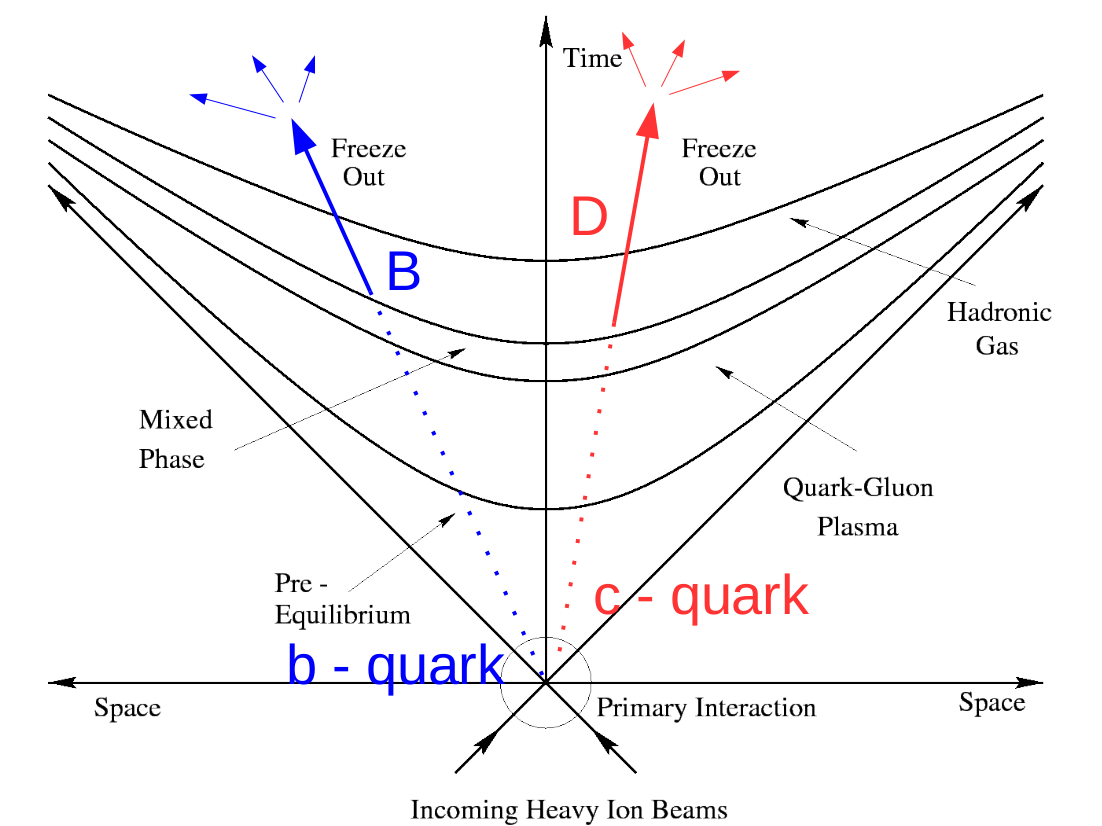
\includegraphics[scale=0.21]{st_cone_hf.png}}

\put(185,245){\captionsetup{labelformat=empty}
\begin{minipage}[t]{0.44\linewidth}
\begin{block}{}
\begin{center}
Gli \textit{heavy flavours} (quark pesanti $c$ e $b$) \\a causa dell'elevata massa 
\[m_c \simeq 1.5 \text{ GeV/c}^2, \text{ } m_b \simeq 4.5 \text{ GeV/c}^2\]
vengono prodotti nella fase iniziale della collisione (\textit{fase di pre-equilibrio}) 
\[\tau_{prod} \sim \frac{\hslash}{m_{b,c}} \sim 0.05-0.1 \text{ fm/c} \]
\end{center}
\end{block}
\end{minipage}}

\put(-5,90){\captionsetup{labelformat=empty}
\begin{minipage}[t]{0.55\linewidth}
\begin{center}
Se nella collisione si crea un mezzo deconfinato (\textit{Quark-Gluon Plasma}), gli heavy flavours interagiscono con esso perdendo energia a causa di scattering elastici con i partoni del mezzo stesso e per radiazione di gluoni (\textit{gluonsstrahlung})
\[\langle \Delta E \rangle \propto \alpha_s C_R \hat{q}L^2\]
\end{center}
\end{minipage}}

\put(230,75){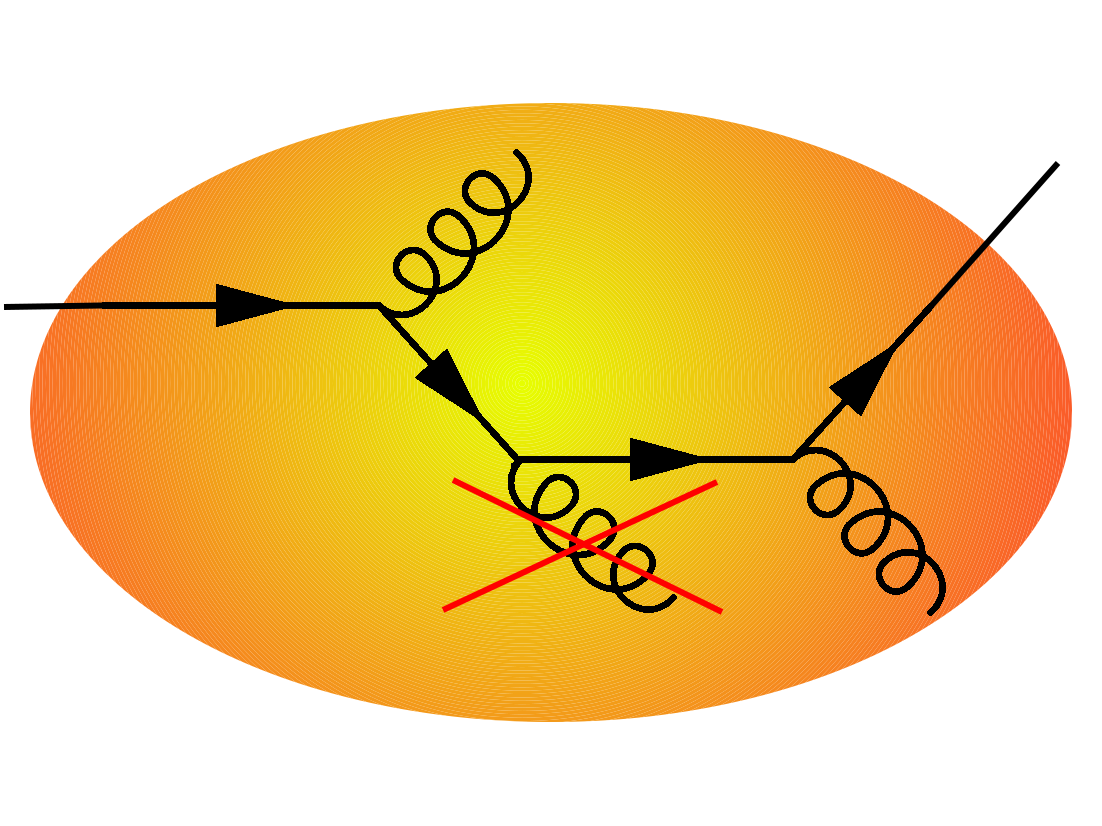
\includegraphics[scale=0.065]{energy_loss.png}}

\put(200,70){\captionsetup{labelformat=empty}
\begin{minipage}[t]{0.4\linewidth}
\begin{center}
La radiazione di gluoni dipende dalla massa del quark, in particolare risulta soppressa per 
\[\theta < \frac{M_q}{E_g} \hspace{2cm}\] 
\end{center}
\end{minipage}}

\put(270,30){\captionsetup{labelformat=empty}
\begin{minipage}[t]{0.4\linewidth}
\textcolor{blue}{DEAD CONE \\EFFECT}
\end{minipage}}

\end{picture} 
\end{frame}

\begin{frame}
\frametitle{\textit{Open heavy flavours} in collisioni p-Pb}
\begin{picture}(320,250)

\put(-5,12){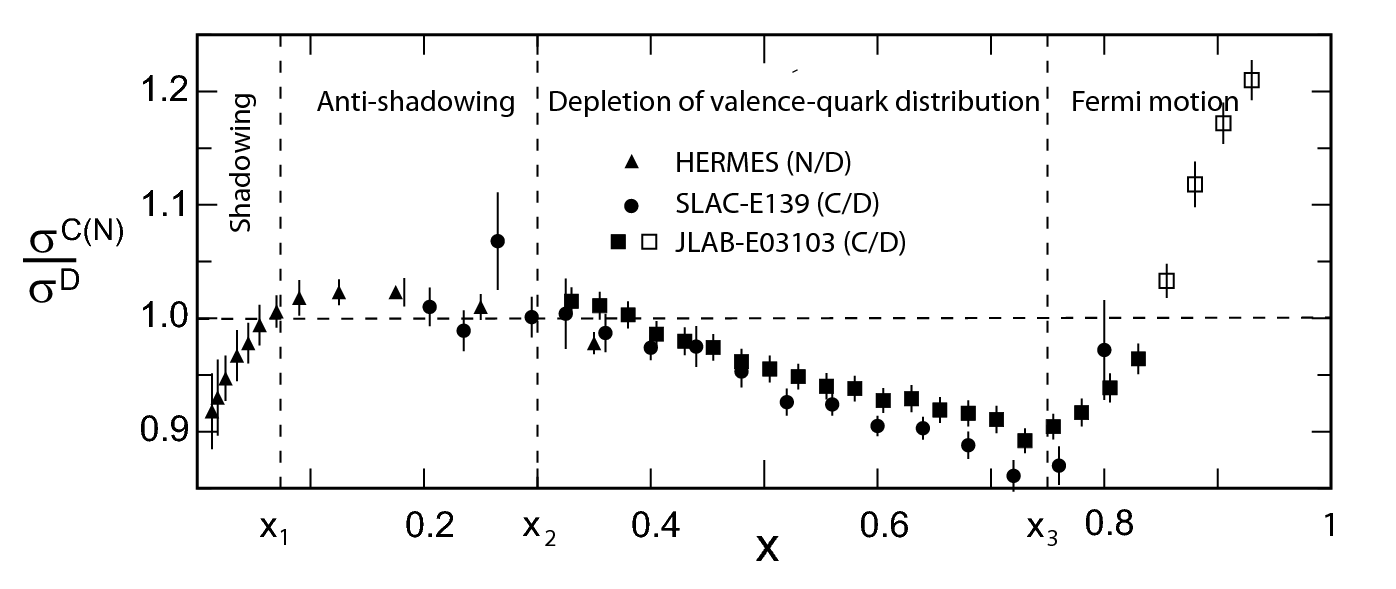
\includegraphics[scale=0.12]{PDF_nuclear_2}}
\put(40,102){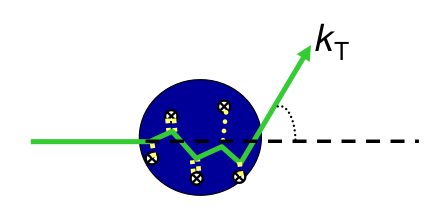
\includegraphics[scale=0.25]{random_walk.png}}
\put(200,90){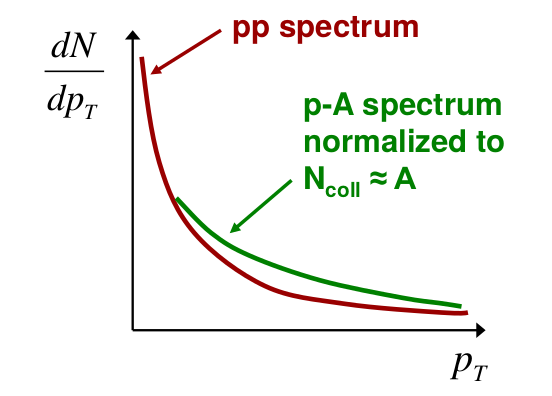
\includegraphics[scale=0.25]{cronin_enhancement.png}}

\put(215,260){\captionsetup{labelformat=empty}
\begin{minipage}[t]{0.3\linewidth}
\begin{block}{\centering \textit{Open heavy flavours}}
\centering
\setlength\abovedisplayskip{0pt}
Adroni formati da un quark pesante ($c$ o $b$) e uno o più quark leggeri
 \end{block}
\end{minipage}}

\put(0,235){\captionsetup{labelformat=empty}
\begin{minipage}[t]{0.6\linewidth}
 Nelle collisioni p-Pb non si raggiungono le condizioni\\ per la formazione di un QGP esteso
 $\Rightarrow$ ci permettono\\ di studiare i \textit{Cold Nuclear Matter Effects}\\\vspace{-0.1cm}
 \begin{itemize}
 \color{blue}
  \item Cronin Enhancement
  \vspace{3.35cm}
  \item Modifica delle PDF in presenza di materia nucleare
 \end{itemize}
\end{minipage}}

\put(10,185){\captionsetup{labelformat=empty}
\begin{minipage}[t]{0.5\linewidth}
Le collisioni multiple dei partoni del proiettile con i nucleoni del nucleo prima dell'\textit{hard scattering} determinano uno \textit{shift} dello spettro a più alti valori di momento trasverso
\end{minipage}}

\put(170,70){\captionsetup{labelformat=empty}
\begin{minipage}[t]{0.58\linewidth}
Si possono distringuere quattro regioni:
\begin{itemize}
 \item $x \lesssim 0.1$ $\rightarrow$ \textit{shadowing region} 
 \item $0.1 \lesssim x \lesssim 0.2$ $\rightarrow$ \textit{anti-shadowing region} 
 \item $0.2 \lesssim x \lesssim 0.8$ $\rightarrow$ \textit{EMC effect} 
 \item $x \gtrsim 0.8$ $\rightarrow$ moto di Fermi
\end{itemize}
\end{minipage}}

\end{picture} 
\end{frame}

\section{ALICE}
\begin{frame}
\frametitle{A Large Ion Collider Experiment}
\begin{picture}(320,250)

\put(0,80){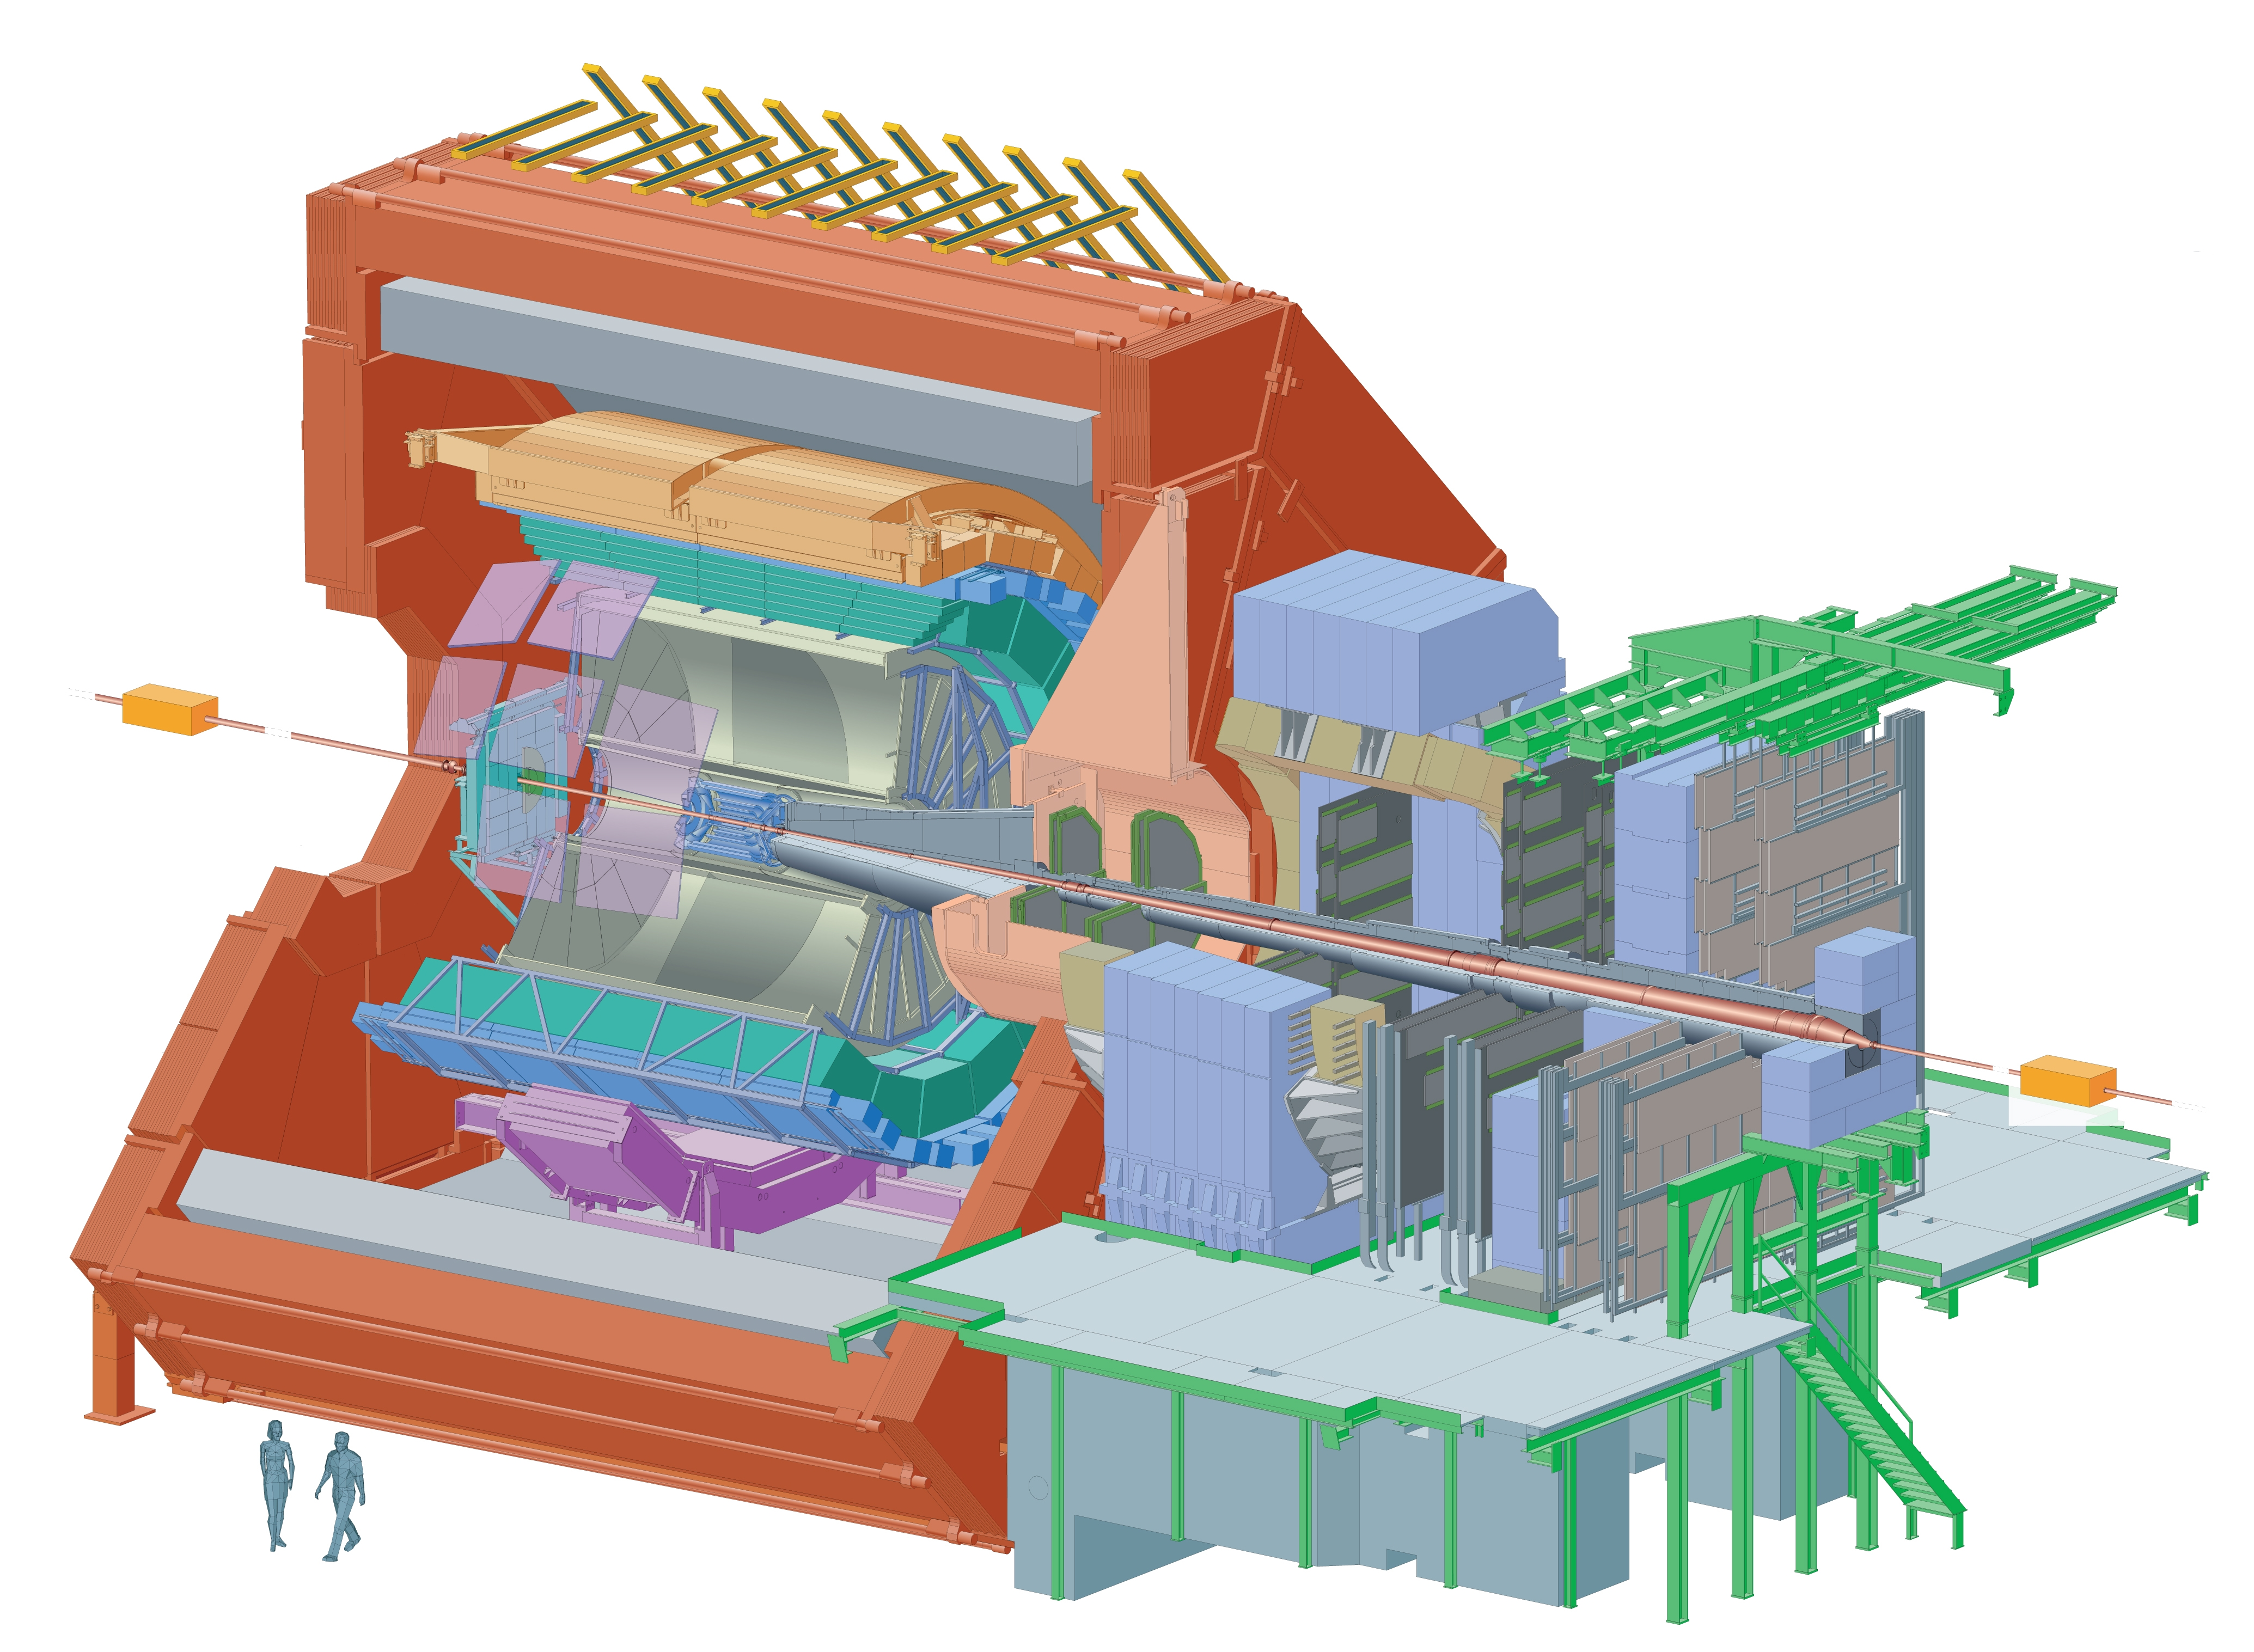
\includegraphics[scale=0.055]{2012-Aug-02-ALICE_3D_v0.jpg}}
\put(10,10){\fcolorbox{red}{white}{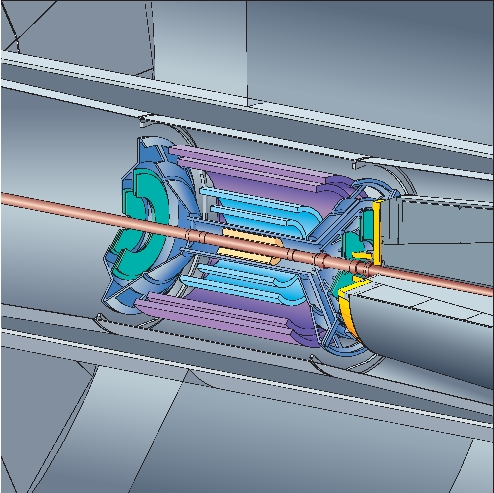
\includegraphics[scale=0.18]{2012-Aug-02-ALICE_3D_ITS}}}
\put(225,160){\fcolorbox{verdebbello}{white}{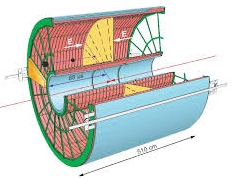
\includegraphics[scale=0.5]{TPC.jpeg}}}
\put(235,20){\fcolorbox{blue}{white}{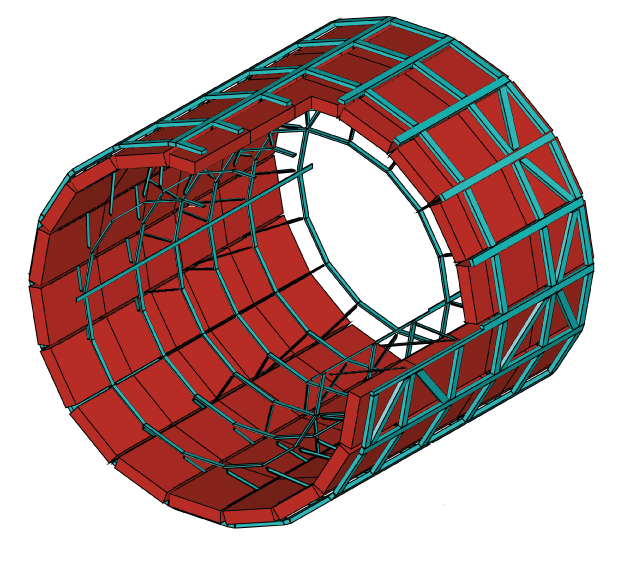
\includegraphics[scale=0.13]{TOF.png}}}

\put(50,80){
\begin{tikzpicture}[->]
\draw[draw=red,solid,line width=0.3mm] (0, 0) -- + (-0.75,-2.8);
\end{tikzpicture}}

\put(95,175){
\begin{tikzpicture}[->]
\draw[draw=verdebbello,solid,line width=0.3mm] (0, 0) -- + (4.3,1);
\end{tikzpicture}}

\put(95,80){
\begin{tikzpicture}[->]
\draw[draw=blue,solid,line width=0.3mm] (0, 0) -- + (4.5,-1.8);
\end{tikzpicture}}

\put(80,60){\captionsetup{labelformat=empty}
\begin{minipage}[t]{0.53\linewidth}
 \hspace{0.1cm} \fcolorbox{red}{white}{{Inner Tracking System}}
\small
\begin{itemize}
\item 2 layer Silicon Pixel Detector
 \item 2 layer Silicon Drift Detector
 \item 2 layer Silicon Strip Detector
\end{itemize}
\end{minipage}}

\put(241,105){\captionsetup{labelformat=empty}
\begin{minipage}[t]{0.53\linewidth}
 \hspace{0.1cm} \fcolorbox{blue}{white}{{Time of Flight}}
\end{minipage}}

\put(230,145){\captionsetup{labelformat=empty}
\begin{minipage}[t]{0.53\linewidth}
 \hspace{0.1cm} \fcolorbox{verdebbello}{white}{{Time Projection Chamber}}
\end{minipage}}

\end{picture} 
\end{frame}

\section{Introduzione all'analisi}
\begin{frame}
\frametitle{Introduzione all'analisi dei mesoni D$^+$}
\begin{picture}(320,250)

\put(25,235){\captionsetup{labelformat=empty}
\begin{minipage}[t]{0.85\linewidth}
\begin{block}{\centering Campione di dati}
\centering
\fontsize{10}{14}\selectfont
L'analisi è stata svolta su un campione di dati acquisiti in collisioni p-Pb a $\sqrt{s_{NN}}=5.02$ TeV dalla Collaborazione ALICE\\
$\Rightarrow$ $\sim$ 100 milioni di eventi \textit{Minimum Bias}\\
\end{block}
\end{minipage}}

\put(0,135){\captionsetup{labelformat=empty}
\begin{minipage}[t]{0.95\linewidth}
\fontsize{10}{14}\selectfont
\textcolor{blue}{Outline:}\vspace{0.1cm}
\begin{enumerate}
 \item Strategia per la ricostruzione dei mesoni D$^+$ \\[3mm]
 \item Metodo del fit del parametro di impatto  \\[3mm]
 \item Metodo della variazione dei tagli \\[3mm]
 \item Misura della produzione dei mesoni D$^+$ con pacchetto di ricostruzione di vertici di decadimento basato sul filtro di Kalman
\end{enumerate}

\end{minipage}}

\end{picture} 
\end{frame}

\section{Ricostruzione di mesoni D$^+$}
\begin{frame}
\frametitle{Ricostruzione e selezione di mesoni D$^+$ in ALICE}
\begin{picture}(320,250)

\put(15,40){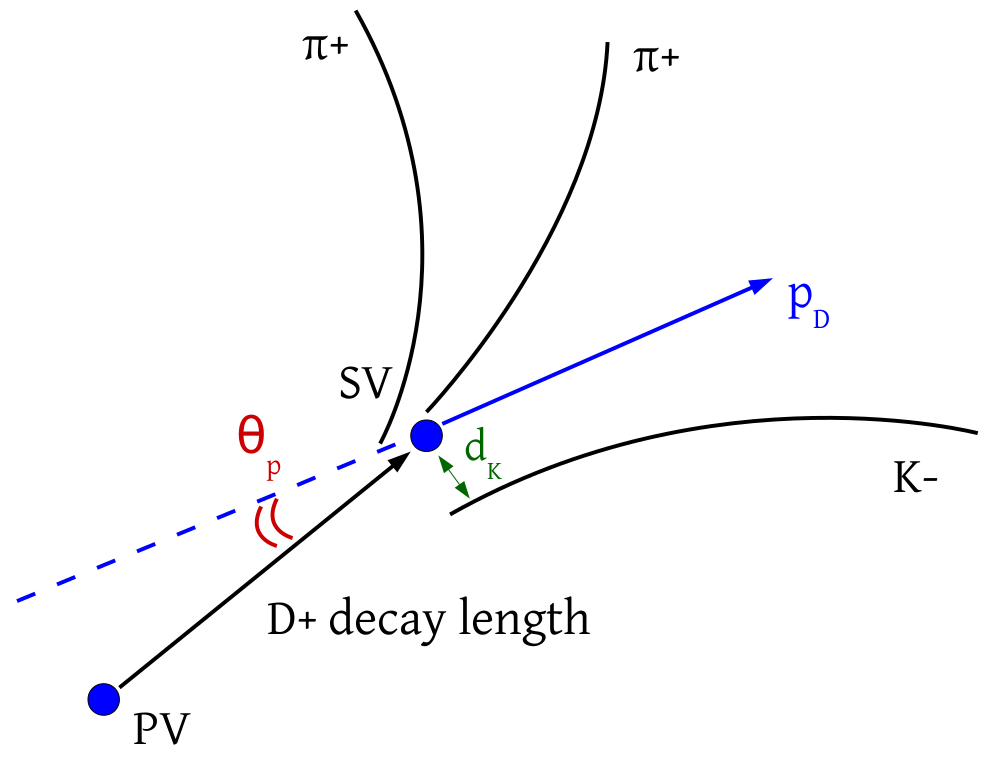
\includegraphics[scale=0.17]{Dplus_sketch.png}}
\put(195,70){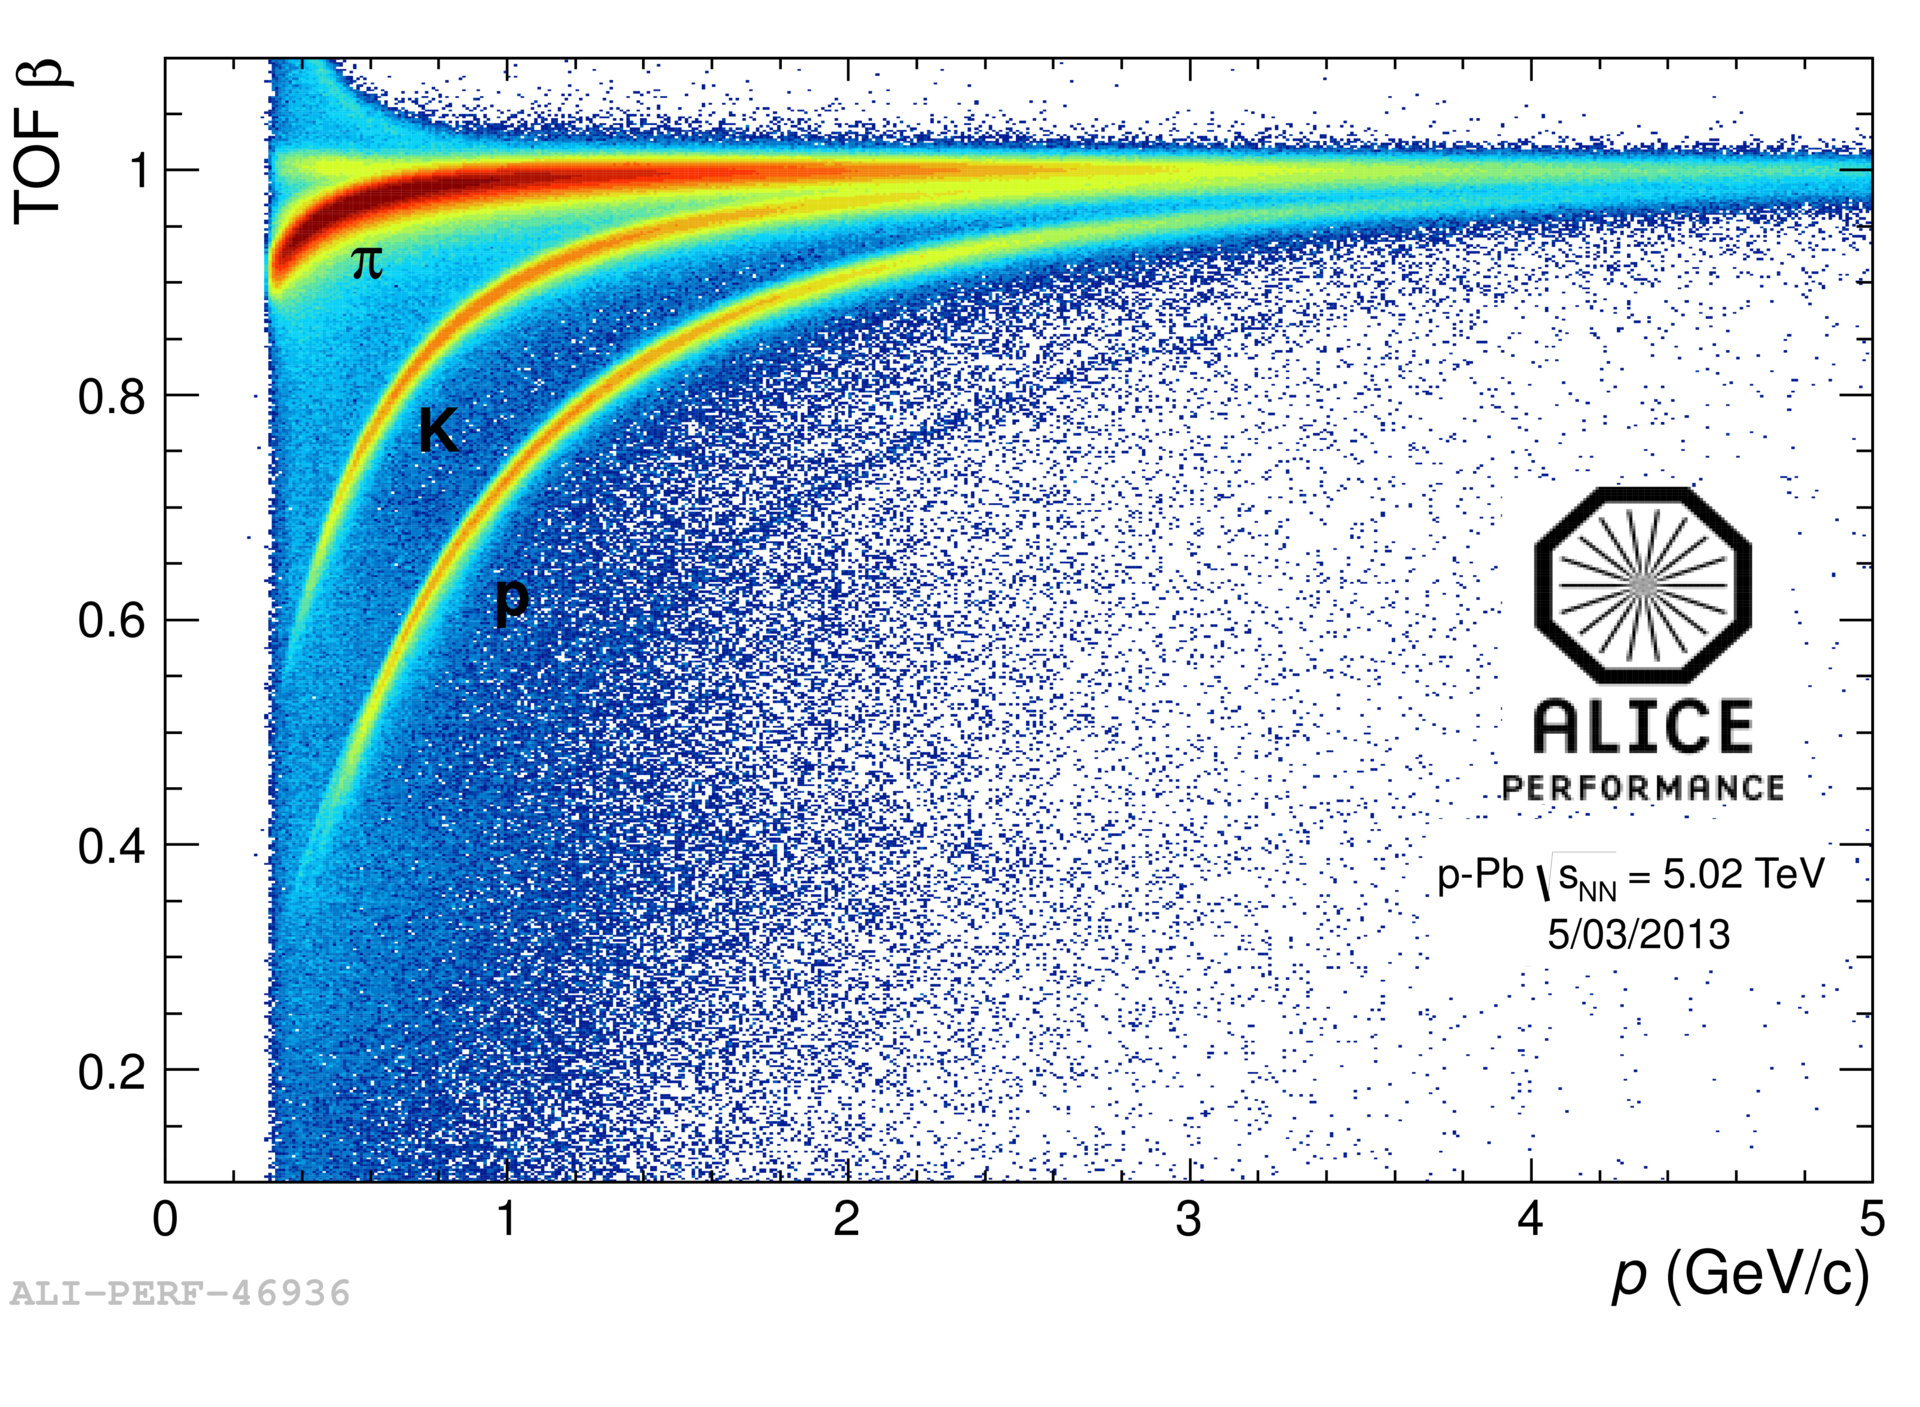
\includegraphics[scale=0.07]{2013-Mar-06-betap_v5.png}}

\put(0,230){\captionsetup{labelformat=empty}
\begin{minipage}[t]{1.\linewidth}
Mesoni D$^+$ ($c\tau = 312\text{ } \mu$m) e coniugati di carica sono ricostruiti nel canale di decadimento adronico
\end{minipage}}

\put(110,227){\captionsetup{labelformat=empty}
\begin{minipage}[t]{0.35\linewidth}
\begin{block}{}
 \setlength\abovedisplayskip{-0.5pt}
\[\text{D}^\pm\rightarrow \text{K}^\mp\pi^\pm\pi^\pm (BR = 9.13\%)\] 
\end{block}
\end{minipage}}

\put(-5,190){\captionsetup{labelformat=empty}
\begin{minipage}[t]{1.\linewidth}
\begin{itemize}
 \item I candidati mesoni D$^+$ vengono ricostruiti combinando tre tracce cariche 
\end{itemize}
\end{minipage}}

\put(-5,177){\captionsetup{labelformat=empty}
\begin{minipage}[t]{0.53\linewidth}
\begin{itemize}
 \item Vengono applicate selezioni sulla qualità delle tracce ricostruite di K$^\pm$ e $\pi^\pm$ e su quantità legate alla topologia del decadimento per ridurre il fondo combinatoriale\\[3.8cm]
 \item Il segnale è estratto con un'\textcolor{blue}{analisi di massa invariante}
\end{itemize}
\end{minipage}}

\put(170,65){\captionsetup{labelformat=empty}
\begin{minipage}[t]{0.53\linewidth}
\begin{itemize}
 \item Per ridurre ulteriormente del fondo viene applicata la \textit{Particle Identification} (PID) nella selezione delle tracce nello stato finale 
\end{itemize}
\end{minipage}}

\end{picture} 
\end{frame}

\section{Mesoni D$^+$ primari e secondari}
\begin{frame}
\frametitle{Mesoni D$^+$ primari e secondari}
\begin{picture}(320,250)

\put(10,25){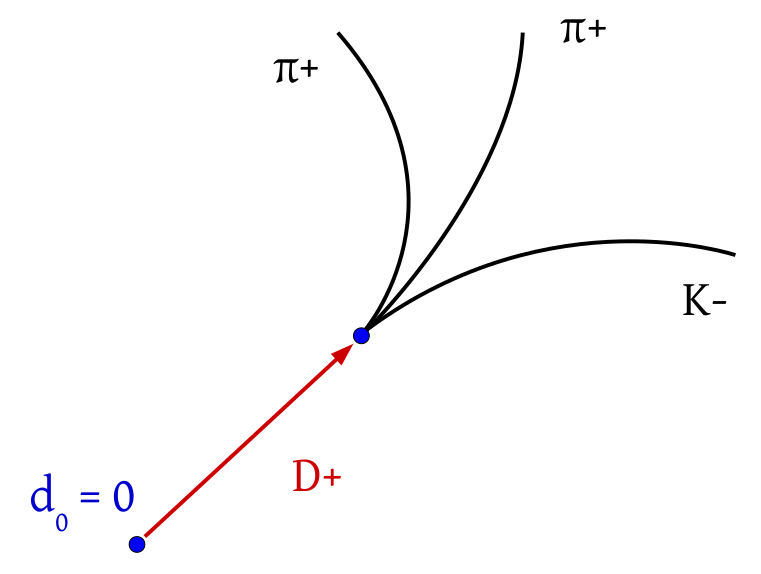
\includegraphics[scale=0.25]{Prompt_sketch.png}}
\put(180,20){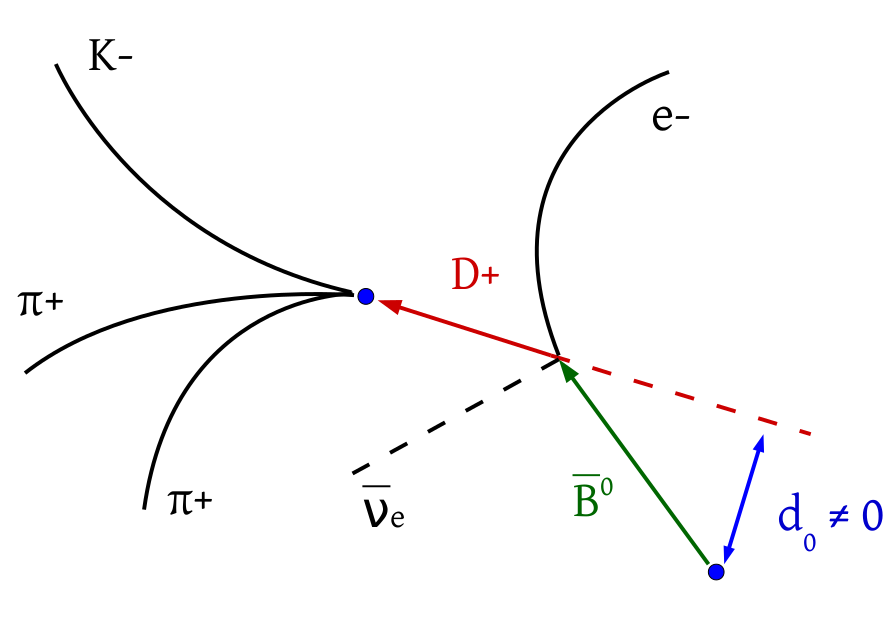
\includegraphics[scale=0.25]{FD_sketch.png}}

\put(10,230){\captionsetup{labelformat=empty}
\begin{minipage}[t]{1.1\linewidth}
\fontsize{9}{11}\selectfont
Per la misura dei mesoni D$^+$ che sono originati da un quark \textit{charm} prodotto nella \\collisione è necessario separare il contributo di D$^+$ prompt dal segnale totale
\end{minipage}}

\put(15,205){\captionsetup{labelformat=empty}
\begin{minipage}[t]{0.4\linewidth}
\begin{block}{\centering D$^+$ primari (\textit{prompt})}
\begin{center}
 Derivano direttamente dall'adronizzazione di un quark $c$ \\
 $c \rightarrow \text{D}^+$
\end{center}
\end{block}
\end{minipage}}

\put(190,205){\captionsetup{labelformat=empty}
\begin{minipage}[t]{0.4\linewidth}
\begin{block}{\centering D$^+$ secondari (\textit{feed-down})}
\begin{center}
 Derivano dal decadimento di un mesone B \\
 $b \rightarrow \text{B} \rightarrow \text{D}^++\text{X}$
\end{center} 
\end{block}
\end{minipage}}

\end{picture} 
\end{frame}

\section{Metodi theory-driven per la misura della frazione di D$^+$ prompt}
\begin{frame}
\frametitle{Metodi \textit{theory-driven} per la misura della frazione di mesoni D$^+$ prompt}
\begin{picture}(320,250)

\put(180,15){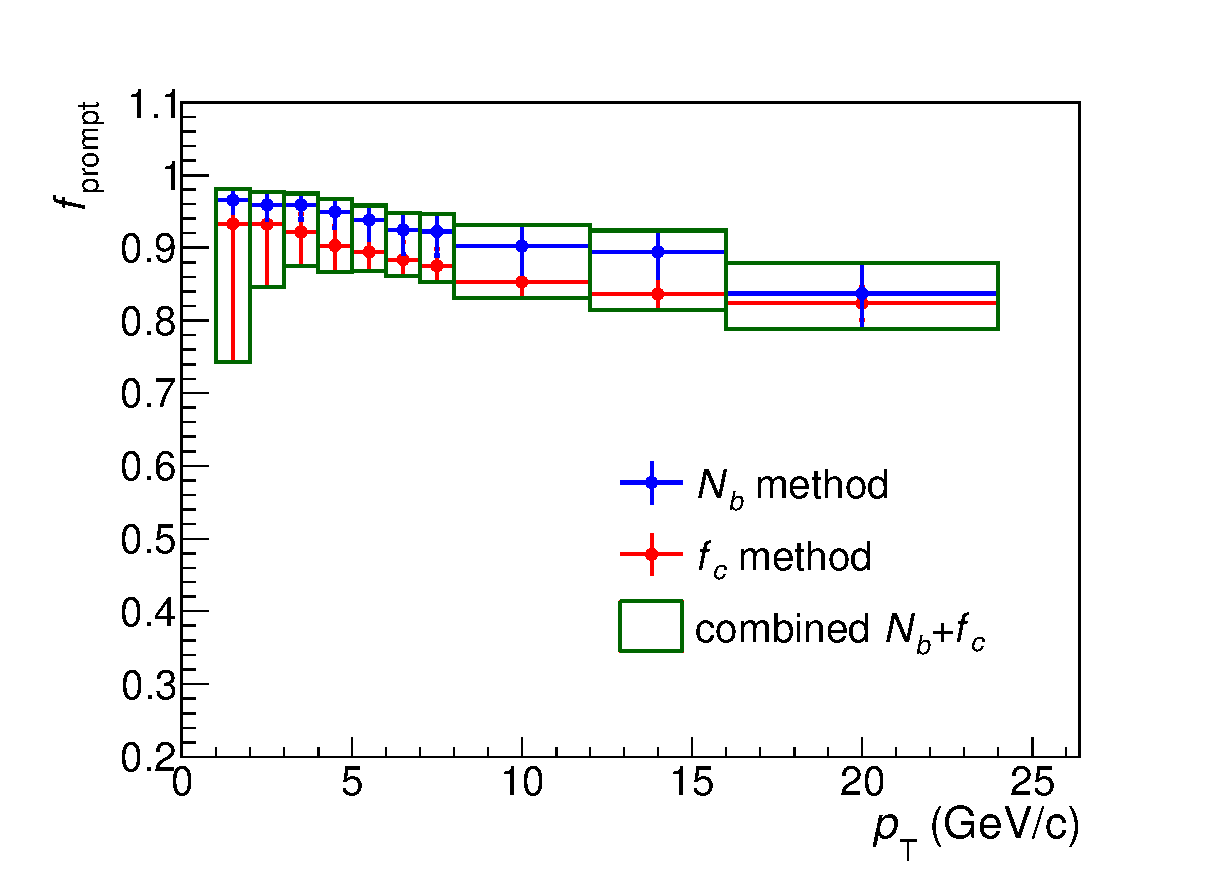
\includegraphics[scale=0.3]{Fprompt_fc_Nb_comp.eps}}

\put(0,235){\captionsetup{labelformat=empty}
\begin{minipage}[t]{1.\linewidth}
La frazione di D$^+$ prompt può essere ottenuta utilizzando metodi \textit{theory-driven}
\end{minipage}}

\put(0,230){\captionsetup{labelformat=empty}
\begin{minipage}[t]{1.\linewidth}
\vspace{0.2cm}
\begin{itemize}
\item Metodo $N_b$ 
 \vspace{-0.2cm}
 \[f_{prompt} = 1-A\cdot \textcolor{blue}{\bigg{(}\frac{d^2\sigma}{d\pt dy}\bigg{)}_{FONLL}^{feed-down}R_{pPb}^{feed-down}(\pt)}\frac{(Acc\times \epsilon)_{feed-down}\cdot\Delta y \Delta\pt \cdot BR \cdot L_{int}}{N_{raw}^{D^\pm}/2}\]
  \item Metodo $f_c$
 \vspace{-0.5cm}
 \[f_{prompt} = \bigg{(} 1+\frac{\textcolor{blue}{\frac{d^2\sigma}{d\pt dy}_{FONLL}^{feed-down}}\cdot(Acc\times \epsilon)_{feed-down}\cdot\textcolor{blue}{R_{pPb}^{feed-down}(\pt)}}{\textcolor{blue}{\frac{d^2\sigma}{d\pt dy}_{FONLL}^{prompt}}\cdot(Acc\times \epsilon)_{prompt}\cdot R_{pPb}^{prompt}(\pt)}\bigg{)}^{-1}\]
\end{itemize}
\end{minipage}}

\put(10,125){\captionsetup{labelformat=empty}
\begin{minipage}[t]{0.95\linewidth}
Principali sorgenti di errore sistematico:
\begin{itemize}
 \item Calcolo perturbativo di \textcolor{blue}{$\bigg{(}\frac{d^2\sigma}{d\pt dy}\bigg{)}_{FONLL}$}
 \item \textcolor{blue}{$R_{pPb}^{feed-down}(\pt)$} mai misurato \\[2mm]$\Rightarrow$ necessità di un'assunzione 
\end{itemize}
\end{minipage}}

\put(20,65){\captionsetup{labelformat=empty}
\begin{minipage}[t]{0.35\linewidth}
\begin{block}{Nuclear modification factor}
\setlength\abovedisplayskip{-1pt}
\[R_{pPb} (\pt) = \frac{1}{<N_{coll}>}\frac{dN_{pPb}/d\pt}{dN_{pp}/d\pt}\]
\end{block}
\end{minipage}}

\end{picture} 
\end{frame}

\section{Metodo di fit del parametro di impatto}
\begin{frame}
\frametitle{Metodo di fit del parametro di impatto}
\begin{picture}(320,250)

\put(175,110){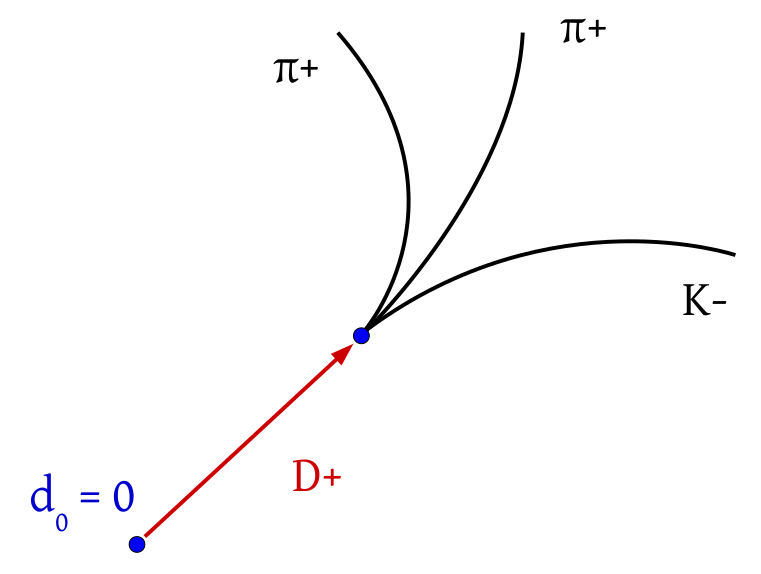
\includegraphics[scale=0.2]{Prompt_sketch.png}}
\put(20,115){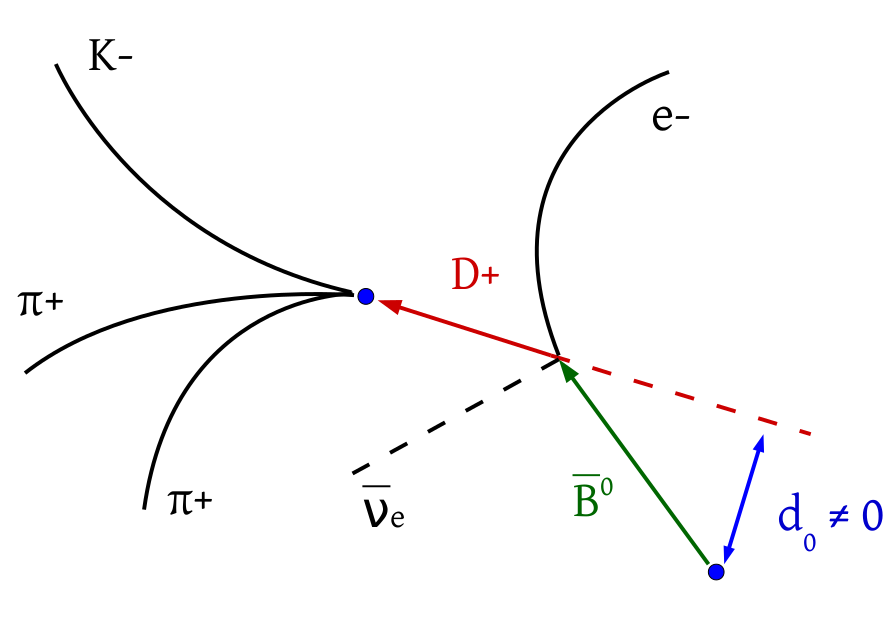
\includegraphics[scale=0.2]{FD_sketch.png}}
\put(230,20){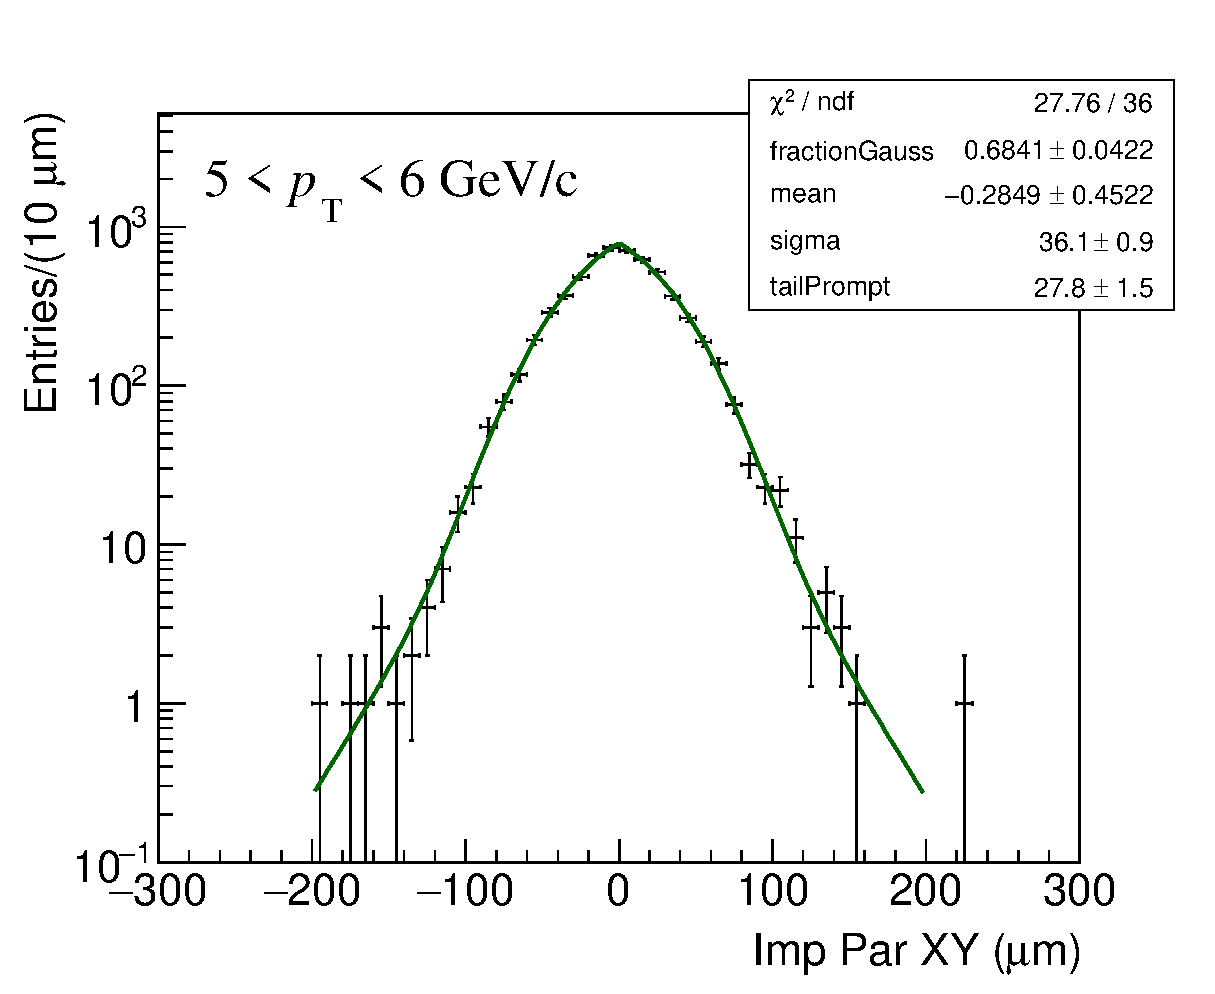
\includegraphics[scale=0.2]{ImpParPrompt_5-6.eps}}

\put(0,232){\captionsetup{labelformat=empty}
\begin{minipage}[t]{0.5\linewidth}
Si basa sulla differenza tra le distribuzioni del parametro di impatto di mesoni D$^+$ prompt e feed-down: 
\end{minipage}}

\put(210,265){\captionsetup{labelformat=empty}
\begin{minipage}[t]{0.35\linewidth}
\begin{block}{\centering Parametro di impatto ($d_0$)}
\setlength\abovedisplayskip{-1pt}
\centering
Minima distanza tra il vertice primario e il prolungamento della traccia del mesone D$^+$ 
\end{block}
\end{minipage}}

\put(5,100){\captionsetup{labelformat=empty}
\begin{minipage}[t]{0.6\linewidth}
\begin{enumerate}
 \item \textcolor{blue}{Determinazione dei \textit{template} (fase di \textit{prefit})}
 \begin{itemize}
  \item Fit delle distribuzioni simulate di mesoni D$^+$ prompt
  \item Fit delle distribuzioni simulate di mesoni D$^+$ feed-down
  \item Fit delle distribuzioni del fondo combinatoriale ottenute dai dati nelle regioni di massa invariante a lato del picco (\textit{side-bands})
 \end{itemize}
 \vspace{0.2cm}
 \item \textcolor{blue}{Fit unbinned dei dati}\\
 La funzione di fit finale è somma dei singoli contributi
\end{enumerate}
\end{minipage}}

\end{picture} 
\end{frame}

\begin{frame}
\frametitle{Fit delle distribuzioni simulate di D$^+$ prompt e feed-down}
\begin{picture}(320,250)

\put(5,130){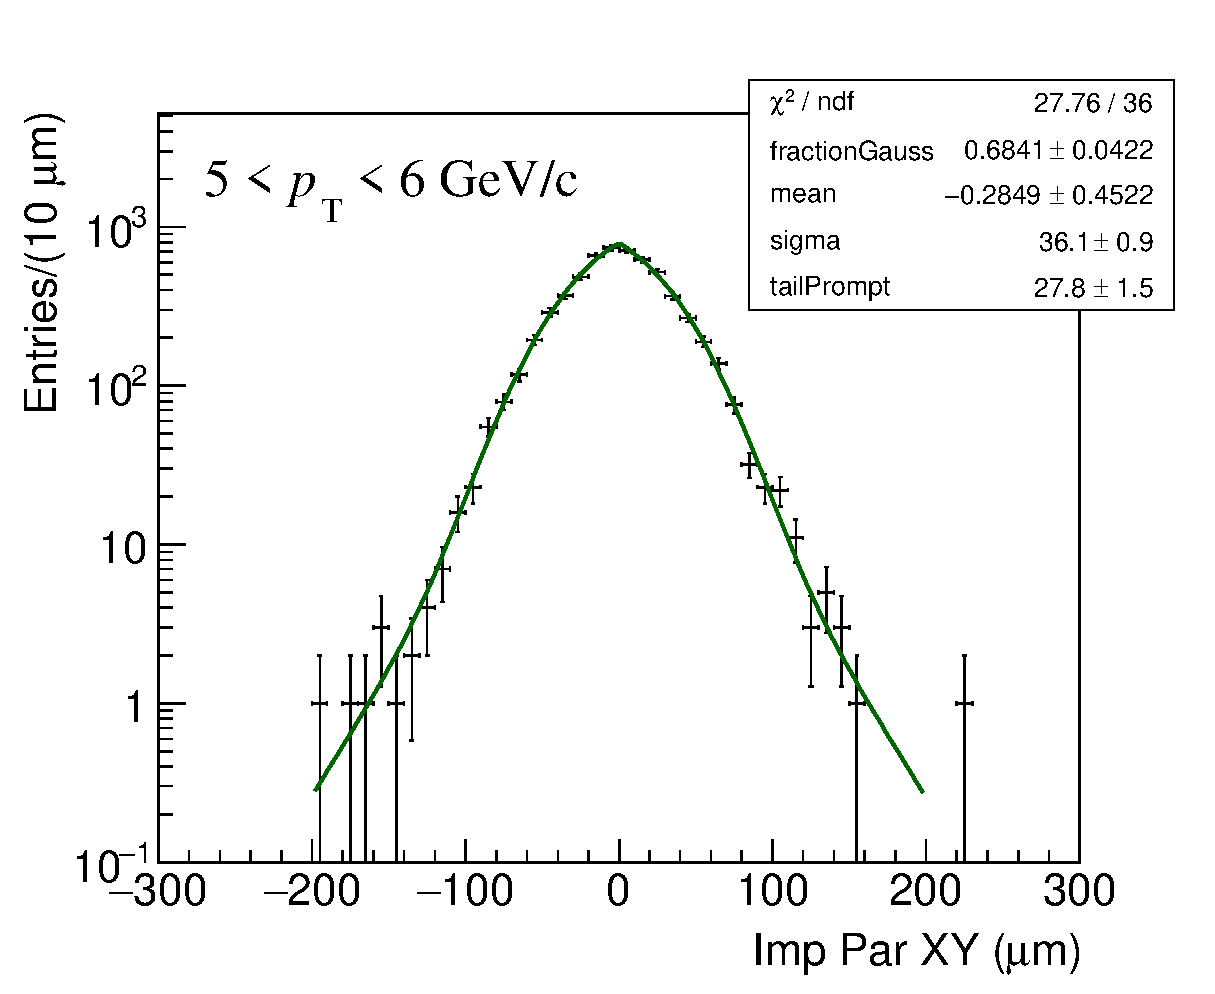
\includegraphics[scale=0.25]{ImpParPrompt_5-6.eps}}
\put(5,15){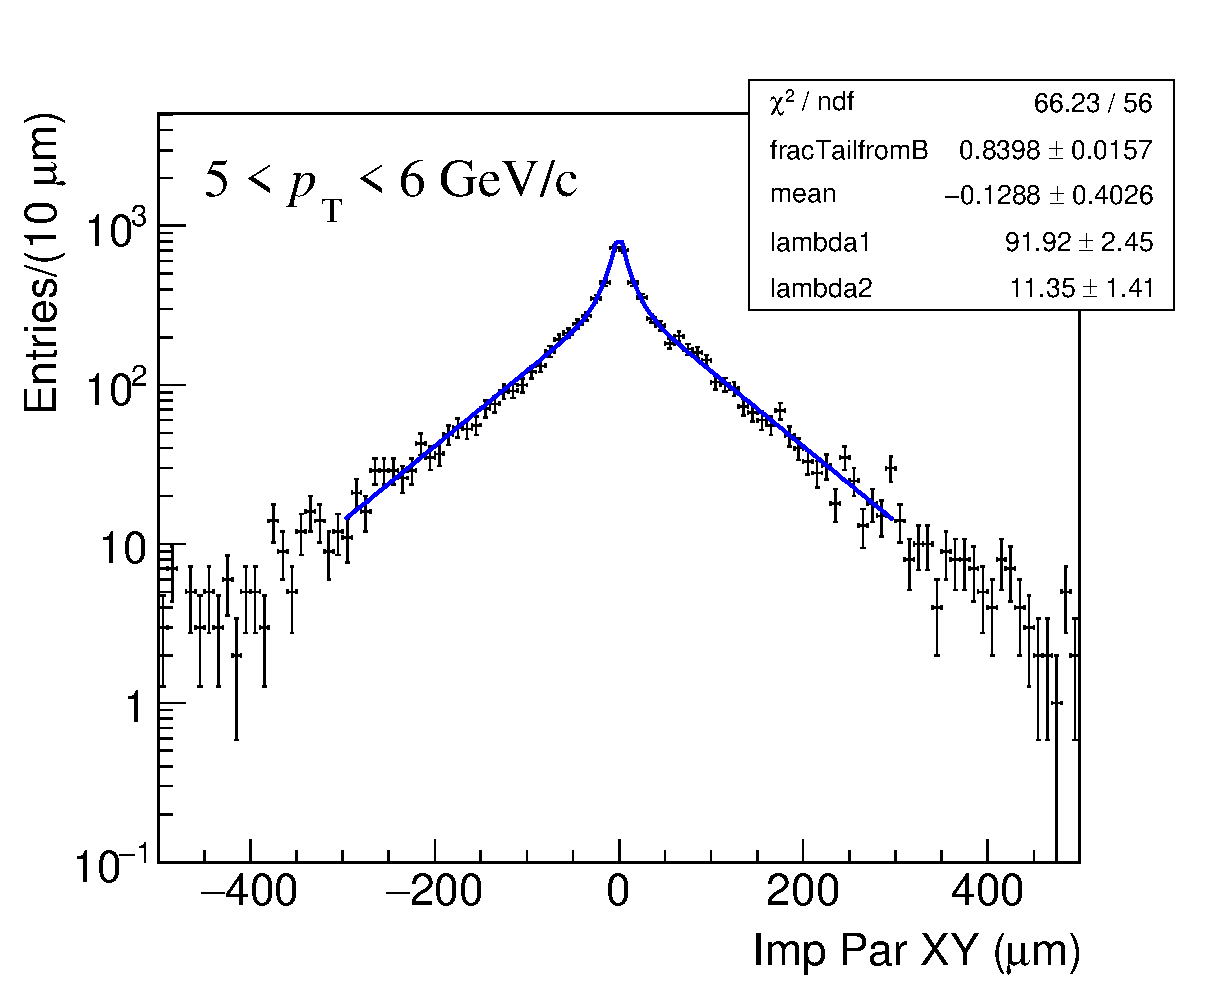
\includegraphics[scale=0.25]{ImpParTrueFD_5-6.eps}}
\put(210,15){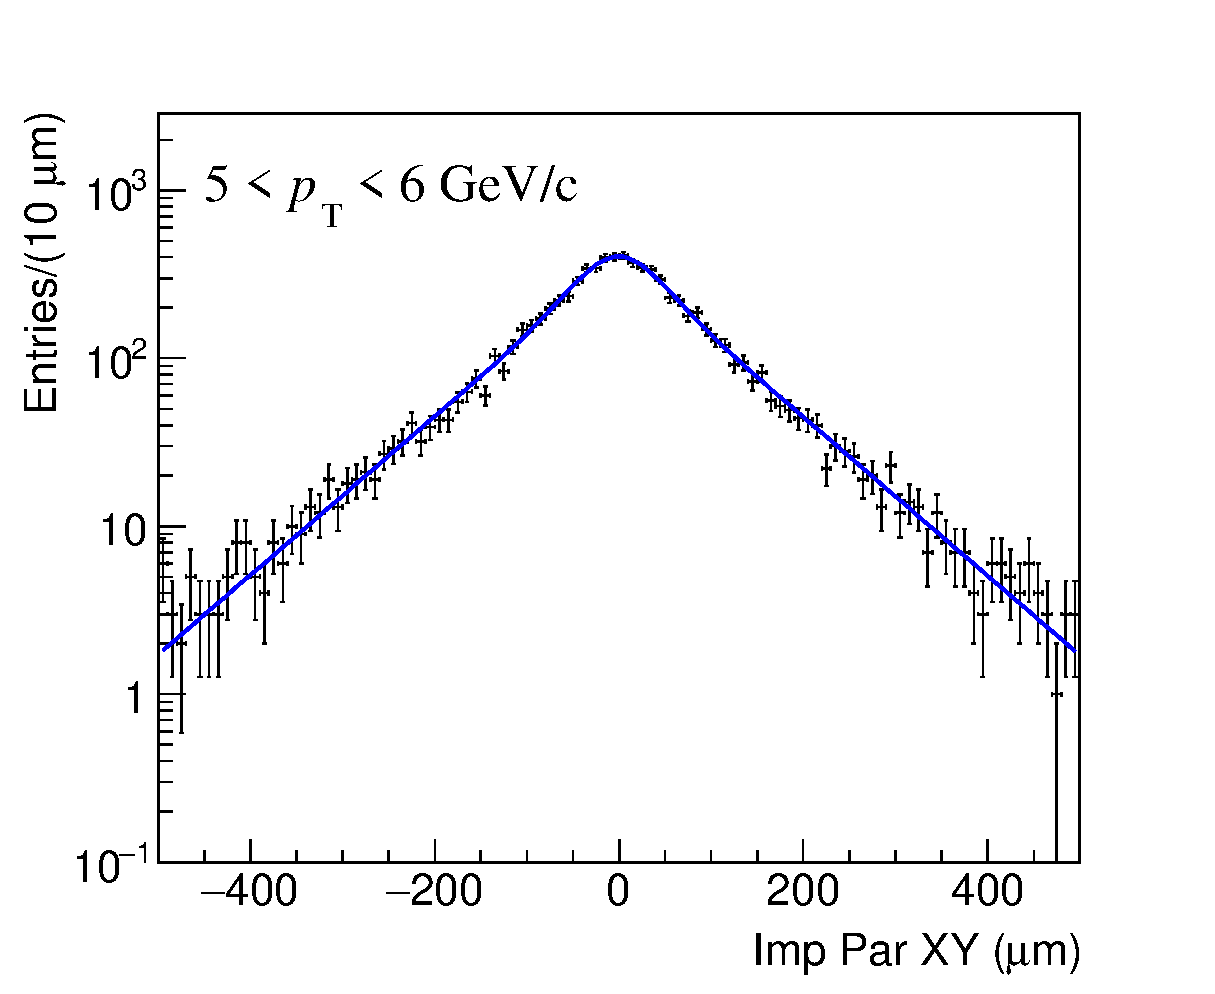
\includegraphics[scale=0.25]{ImpParRecoFD_5-6.eps}}

\put(160,230){\captionsetup{labelformat=empty}
\begin{minipage}[t]{0.5\linewidth}
\textcolor{verdebbello}{D$^+$ prompt}: fit della distribuzione del parametro di impatto \textit{simulato}\\
$\rightarrow$ somma di una Gaussiana e una funzione esponenziale simmetrica rispetto al valor medio
\end{minipage}}

\put(160,170){\captionsetup{labelformat=empty}
\begin{minipage}[t]{0.5\linewidth}
\textcolor{blue}{D$^+$ feed-down}: fit della distribuzione del parametro di impatto \textit{vero}\\
$\rightarrow$ somma di due funzioni esponenziali simmetriche rispetto al valor medio
\end{minipage}}

\put(145,85){
\begin{tikzpicture}[->]
\draw[draw=blue,solid,line width=0.3mm] (0, 0) -- + (1.8,0);
\end{tikzpicture}}

\put(145,65){\captionsetup{labelformat=empty}
\begin{minipage}[t]{0.2\linewidth}
Convoluzione\\[1mm] di \textcolor{blue}{$F^{feed-down}_{true}(d_0^{xy})$}\\[1mm] con \textcolor{verdebbello}{$F^{prompt}(d_0^{xy})$}
\end{minipage}}

\end{picture} 
\end{frame}

\begin{frame}
\frametitle{Fit delle distribuzioni del fondo combinatoriale}
\begin{picture}(320,250)

\put(-5,130){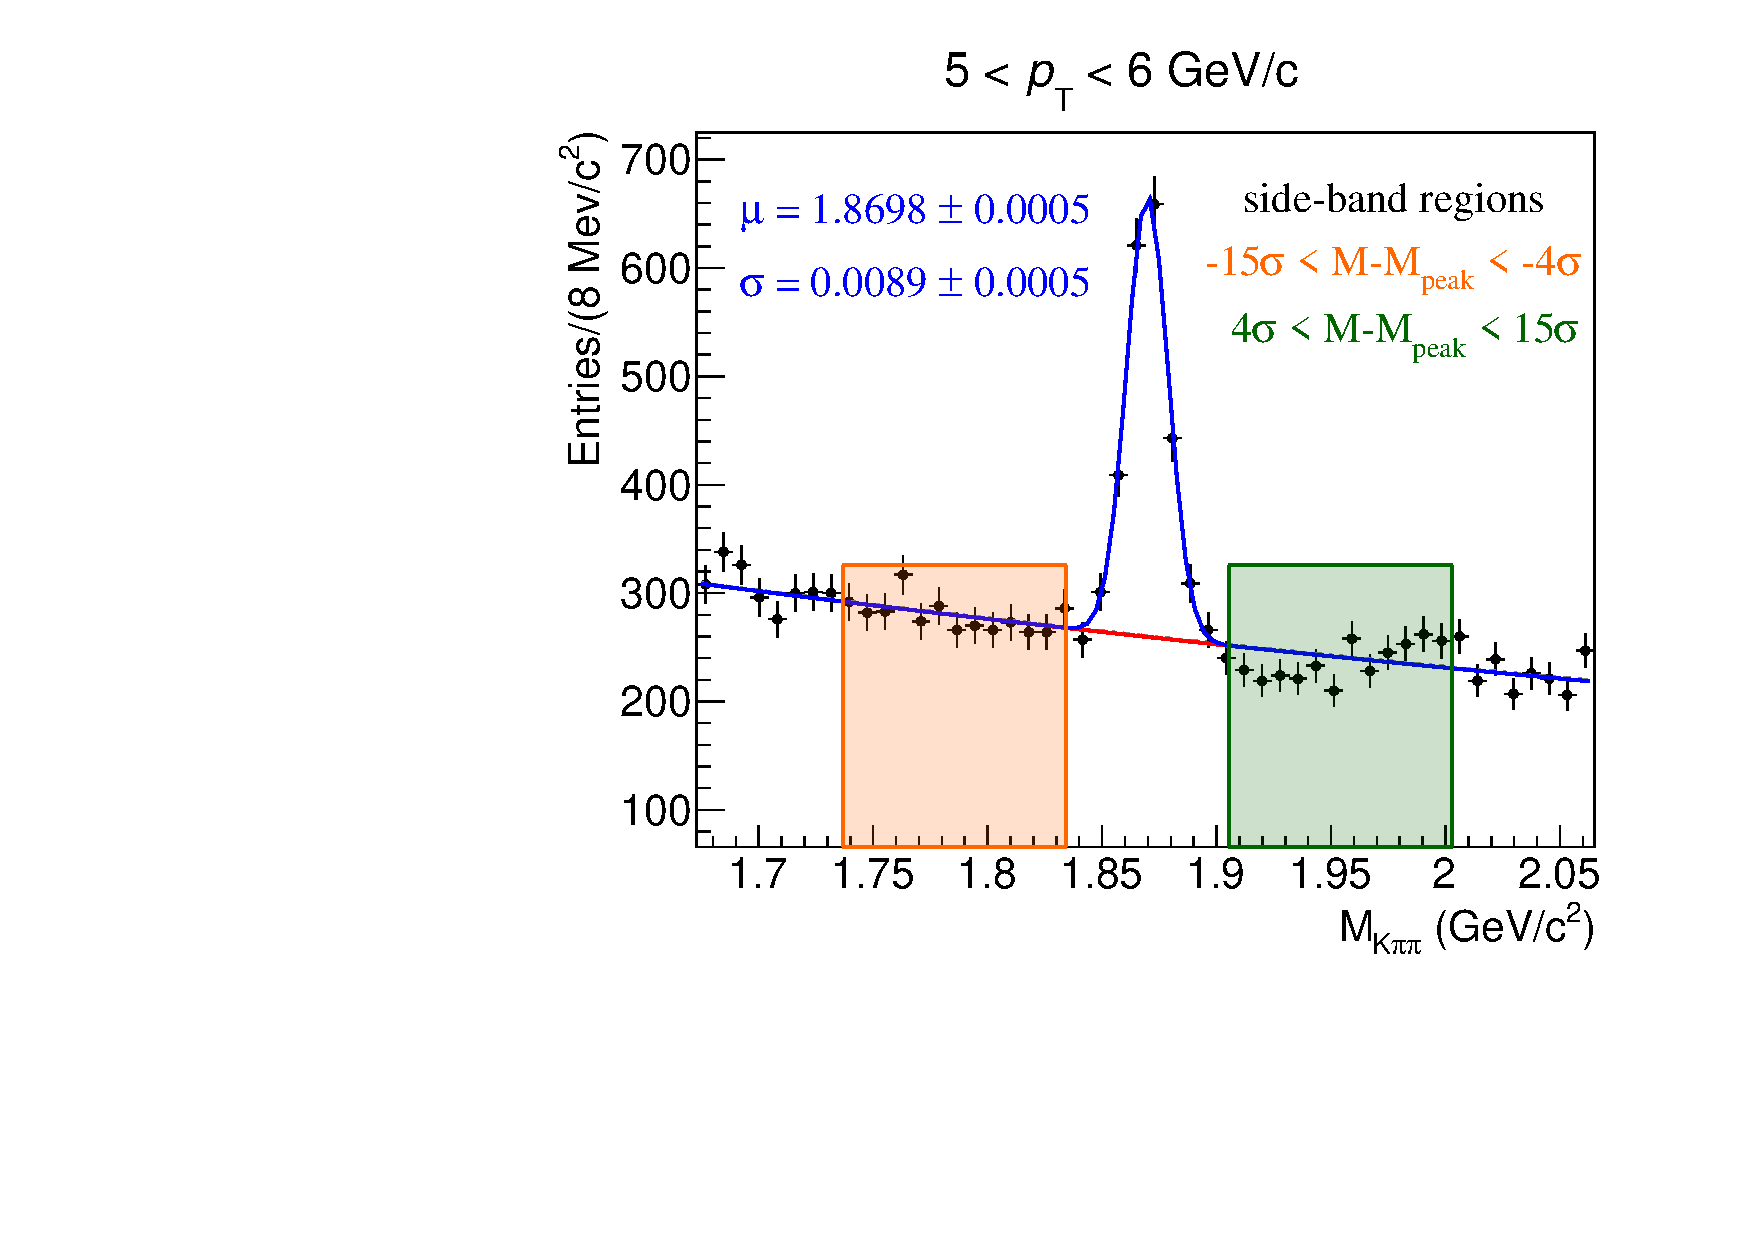
\includegraphics[scale=0.25]{Mass_5-6.pdf}}
\put(175,94){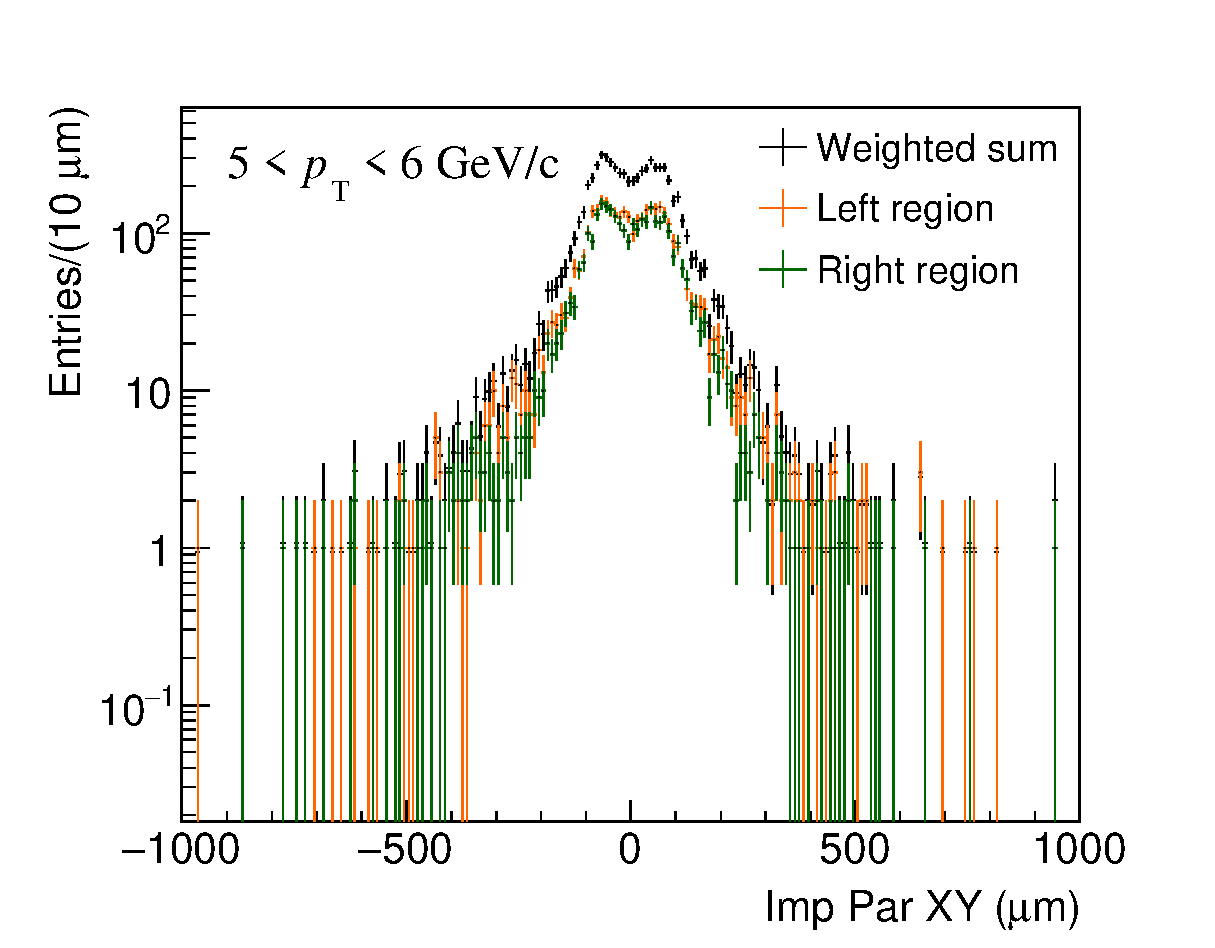
\includegraphics[scale=0.25]{Sidebands_Pt_5-6_NoFit.eps}}
\put(5,10){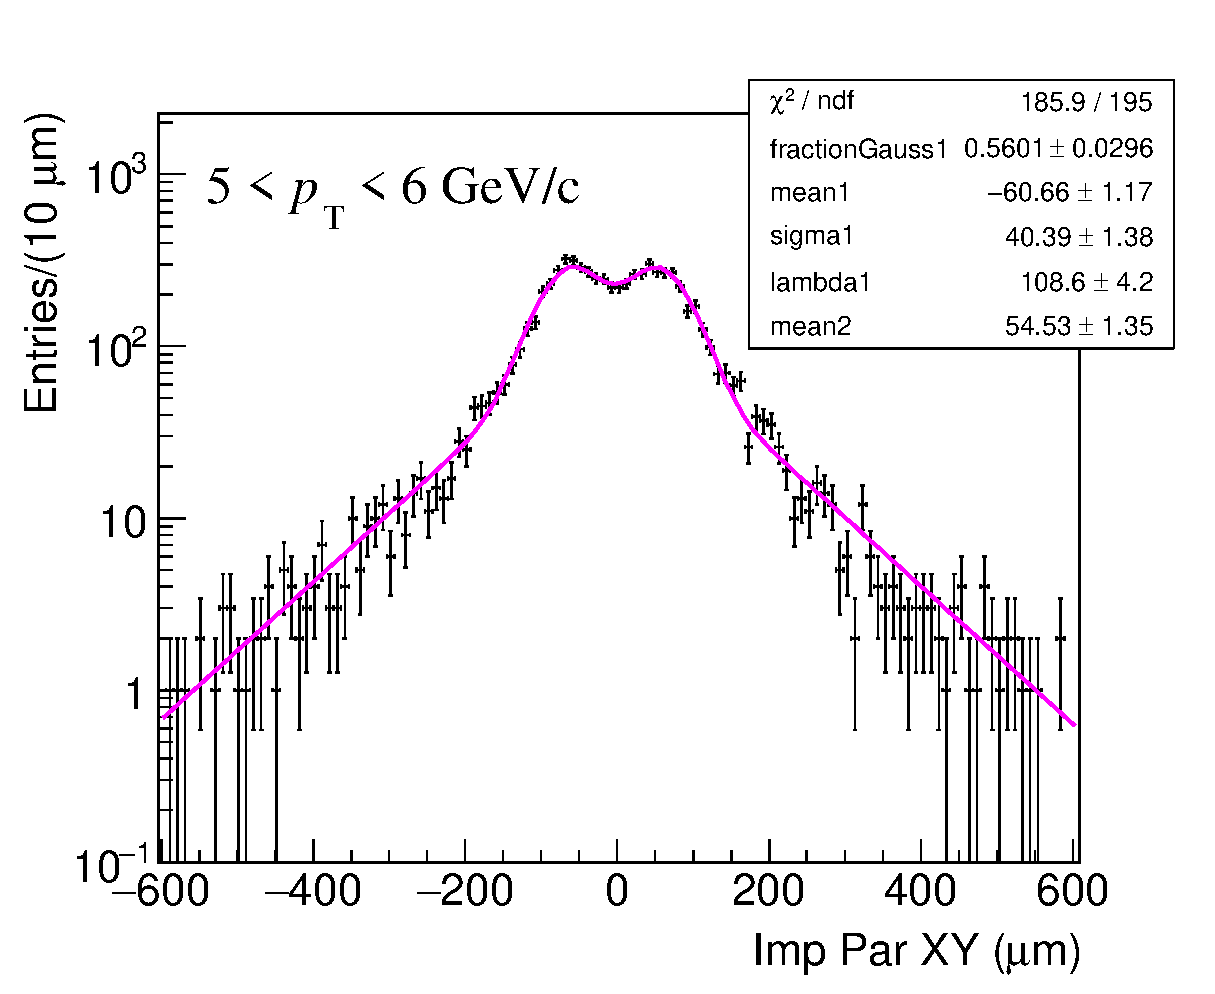
\includegraphics[scale=0.25]{ImpParBkg_5-6.eps}}

\put(103,130){
\begin{tikzpicture}[->]
\draw[draw=verdebbello,solid,line width=0.3mm] (0, 0) -- + (2.7,-0.5);
\end{tikzpicture}}

\put(56.5,145){
\begin{tikzpicture}[->]
\draw[draw=orange,solid,line width=0.3mm] (0, 0) -- + (4.2,-0.8);
\end{tikzpicture}}

\put(160,80){\captionsetup{labelformat=empty}
\begin{minipage}[t]{0.5\linewidth}
\textcolor{magenta}{Fondo combinatoriale}: fit della distribuzione del parametro di impatto ottenuta dalle regioni di massa invariante a lato del picco (\textit{side-bands})
\[4\sigma<|M-M_{peak}|<15\sigma\]
$\rightarrow$ somma di due Gaussiane con code esponenziali, con i parametri uguali a meno dei valori medi
\end{minipage}}

\put(140,250){\captionsetup{labelformat=empty}
\begin{minipage}[t]{0.57\linewidth}
\begin{block}{\centering Fondo combinatoriale}
\centering
Fondo costituito dalla combinazione di tracce scorrelate, non derivanti dal decadimento di mesoni D$^+$ 
\end{block}

\end{minipage}}

\end{picture} 
\end{frame}

\begin{frame}
\frametitle{Fit \textit{unbinned} dei dati}
\begin{picture}(320,250)

\put(5,135){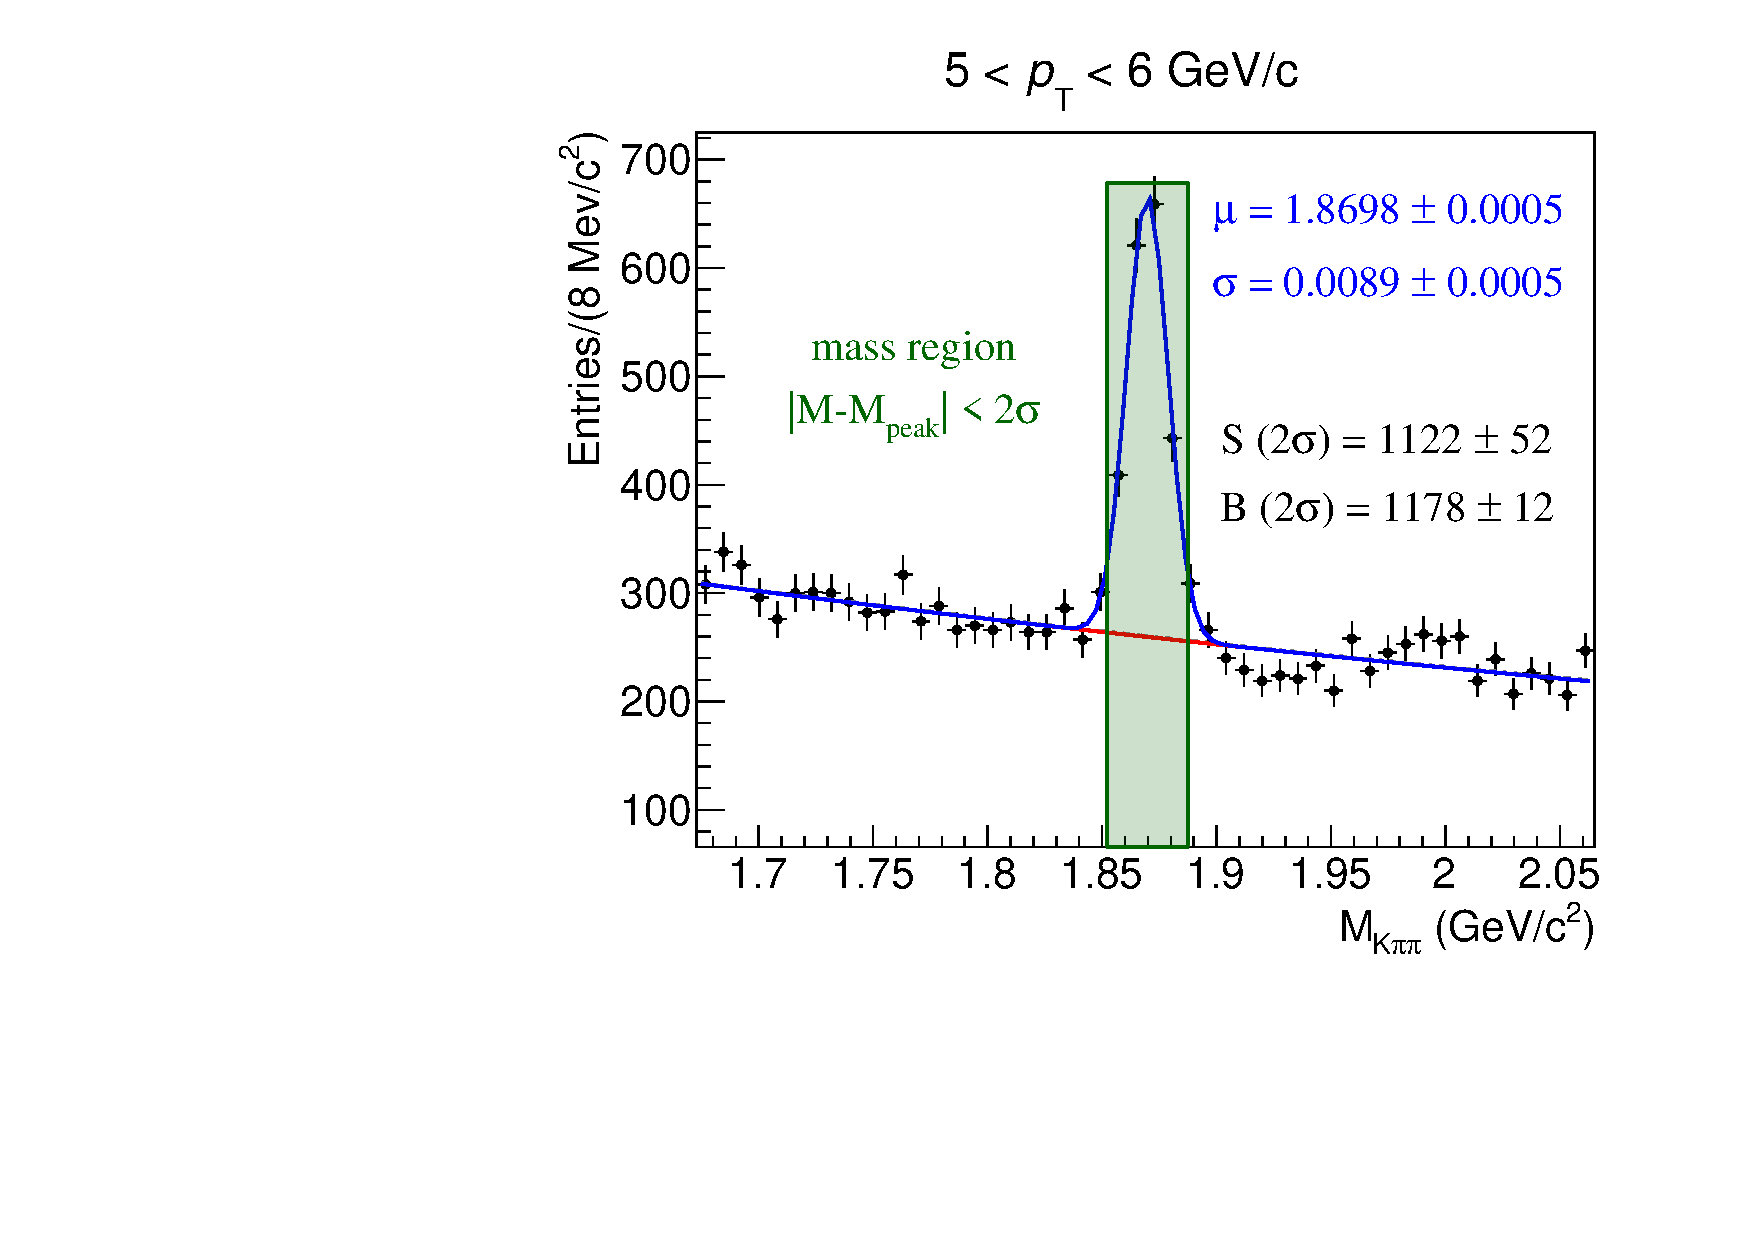
\includegraphics[scale=0.25]{Mass_5-6_fit.pdf}}
\put(150,60){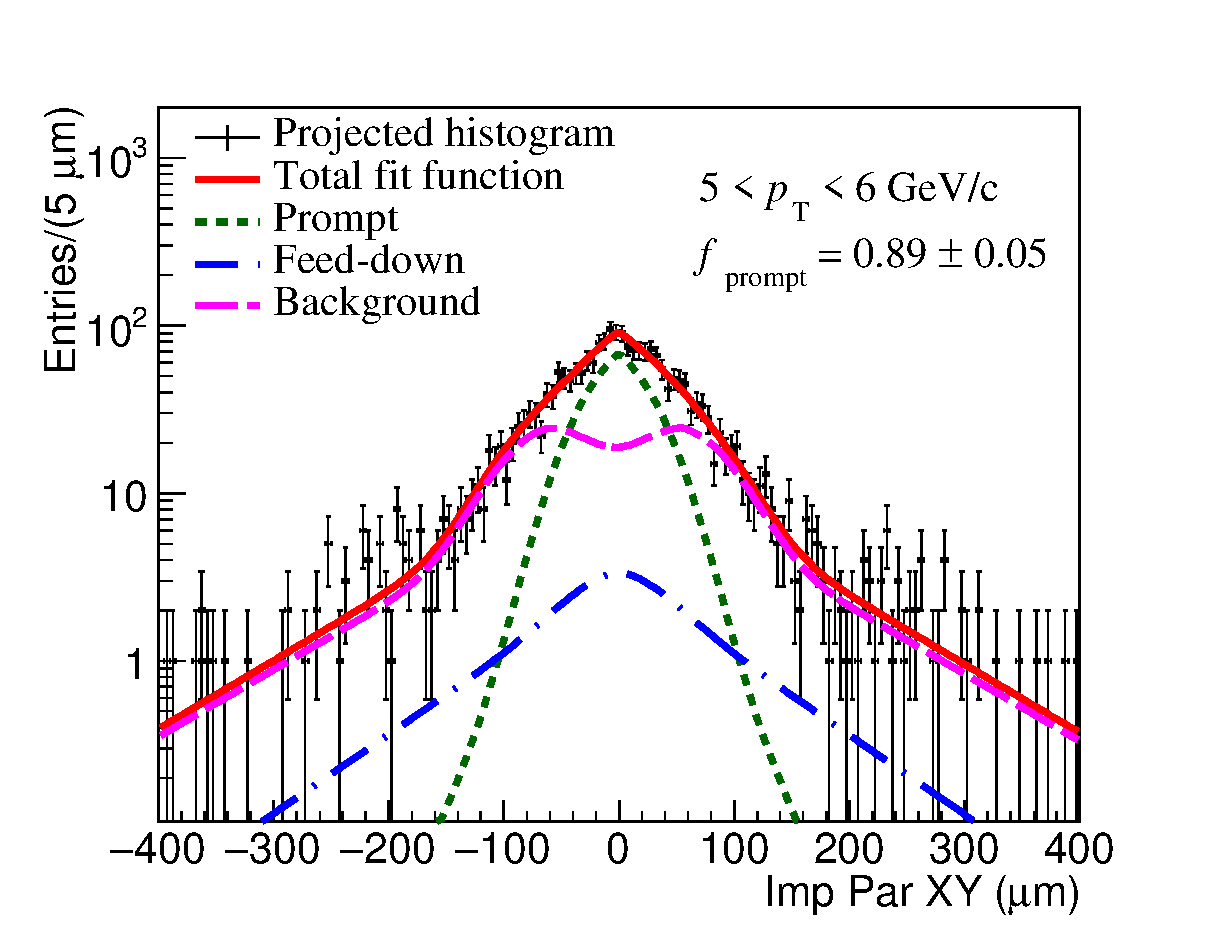
\includegraphics[scale=0.35]{FitUnbinned_5-6_bkg_plot.eps}}

\put(81,120){
\begin{tikzpicture}[->]
\draw[draw=verdebbello,solid,line width=0.3mm] (0, 0) -- + (3.,-2);
\end{tikzpicture}}

\put(160,235){\captionsetup{labelformat=empty}
\begin{minipage}[t]{0.5\linewidth}
\begin{center}
Intervallo di massa invariante considerato
\[|M-M_{peak}|<2\sigma\]
\end{center}
\end{minipage}}

\put(-5,125){\captionsetup{labelformat=empty}
\begin{minipage}[t]{0.45\linewidth}
\begin{itemize}
 \item Parametri liberi: $f_{prompt}, \text{ } \sigma_{prompt}$
 \item $S$ è fissato al valore del segnale ottenuto dal fit della massa invariante (\textit{raw yield})
 \item $N$ è fissato al numero di conteggi
\end{itemize}
\end{minipage}}

\put(15,60){\captionsetup{labelformat=empty}
\begin{minipage}[t]{0.9\linewidth}
 \begin{block}{}
 \setlength\abovedisplayskip{0pt}
\[ \textcolor{red}{F(d_0^{xy})} = N \cdot \bigg\{\frac{S}{N}\bigg{[}f_{prompt}\textcolor{verdebbello}{F^{prompt}(d_0^{xy})}+(1-f_{prompt})\textcolor{blue}{F^{feed-down}_{reco}(d_0^{xy})}\bigg{]}+\frac{N-S}{N}\textcolor{magenta}{F^{bkg}(d_0^{xy})}\bigg\} \]
\end{block}
\end{minipage}}

\end{picture} 
\end{frame}

\begin{frame}
\frametitle{Valutazione degli errori sistematici}
\begin{picture}(320,250)

\put(5,12){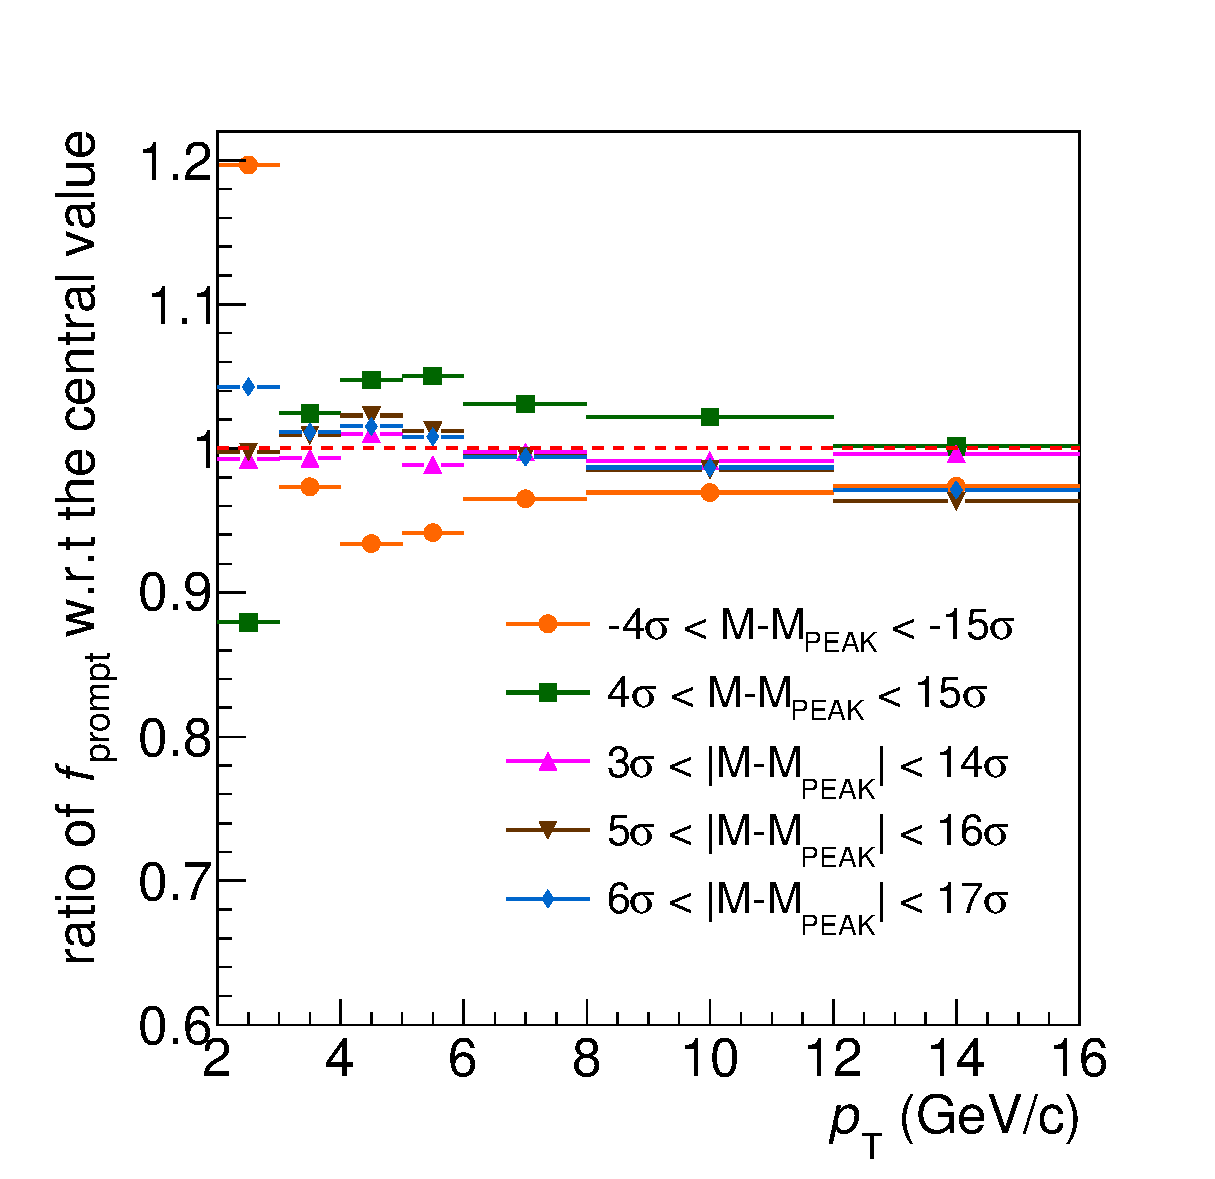
\includegraphics[scale=0.18]{promptfraction_syst_SBtot_ratioonly.eps}}
\put(125,12){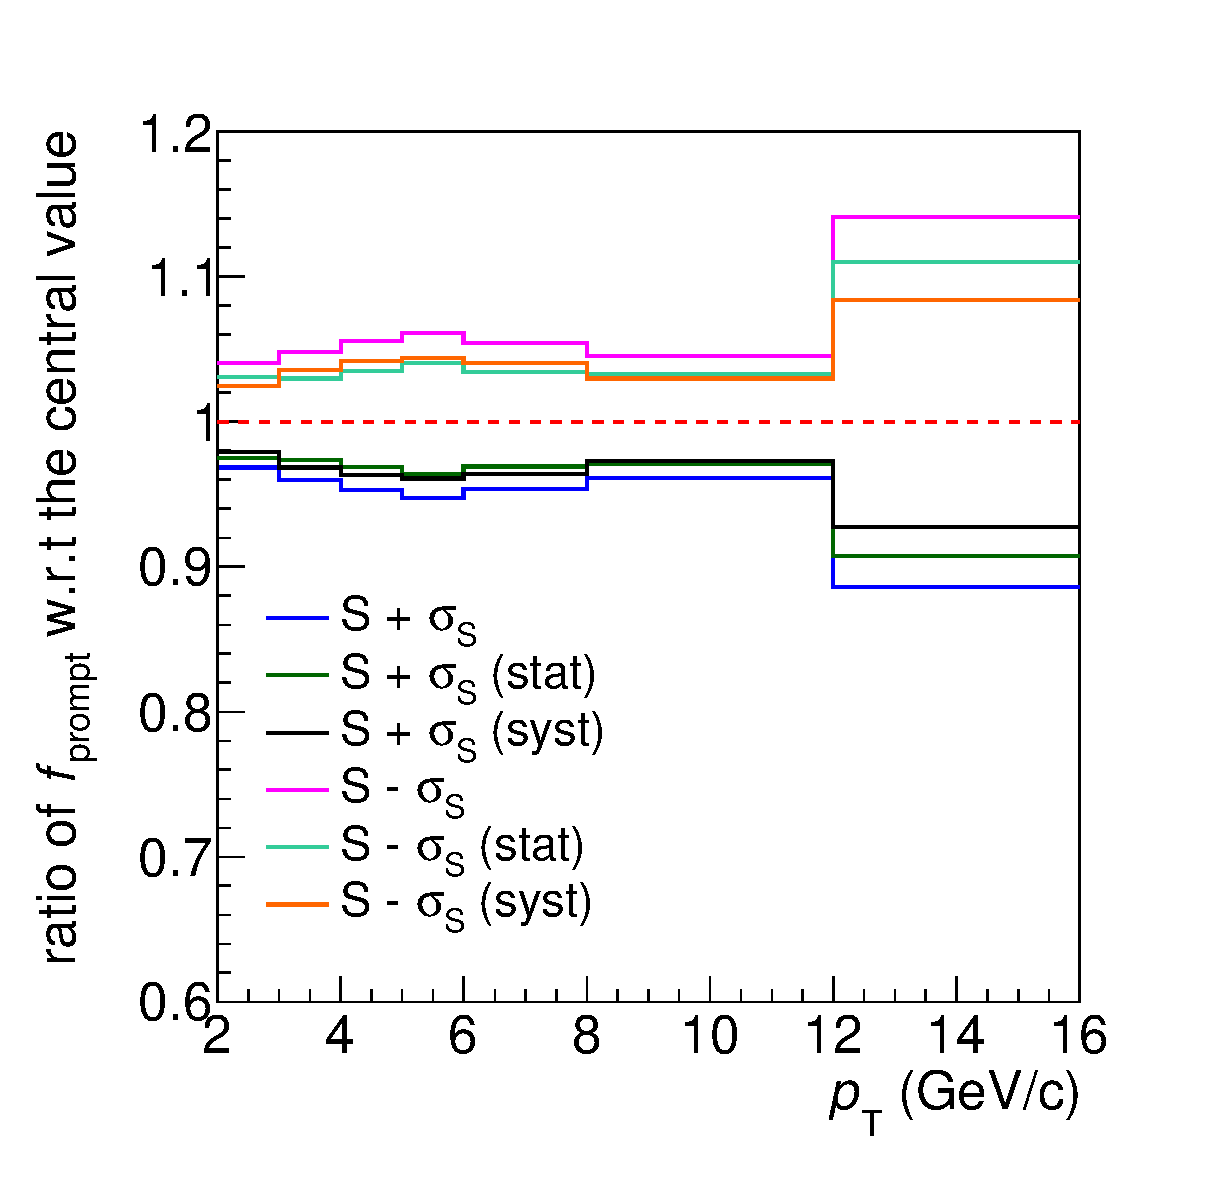
\includegraphics[scale=0.18]{promptfraction_syst_SoverT_onlyratio.eps}}
\put(240,12){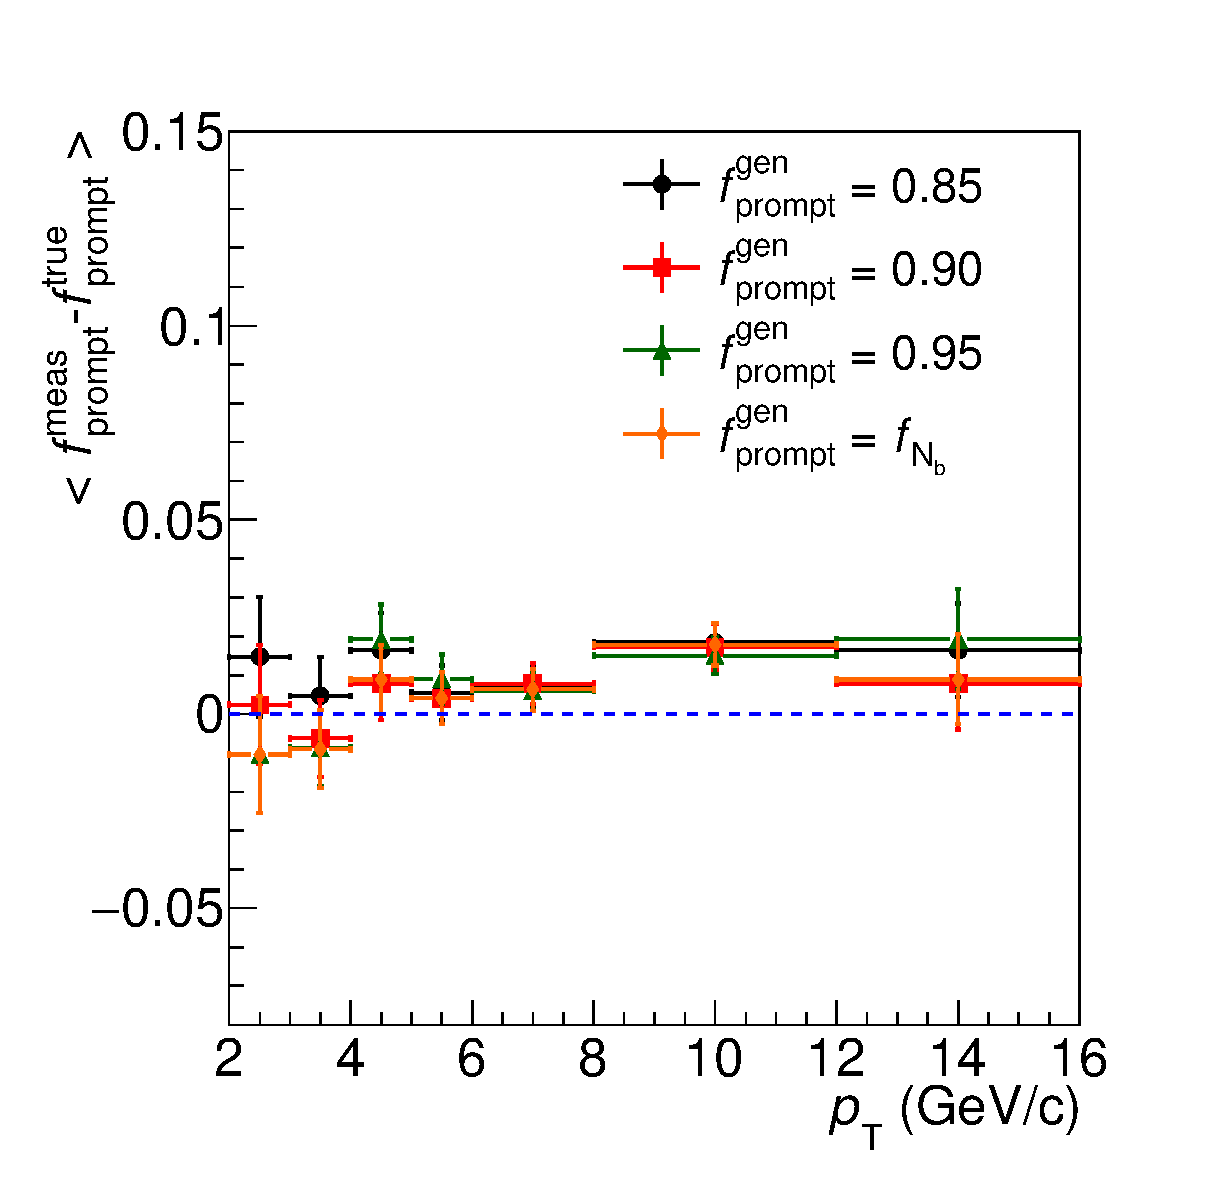
\includegraphics[scale=0.18]{Bias_bkg_freesigma.eps}}

\put(0,235){\captionsetup{labelformat=empty}
\begin{minipage}[t]{1.\linewidth}
Sorgenti di errore sistematico:
\begin{enumerate}
 \item Imperfetta descrizione delle distribuzioni 
 \begin{enumerate}[a)]
  \item Forma delle distribuzioni del parametro di impatto di D$^+$ prompt e feed-down nella simulazione Monte Carlo e del fondo combinatoriale nelle side-bands \\
 \item Forma delle distribuzioni di $\pt$ di mesoni D$^+$ e B generati nella simulazione Monte Carlo \\
 \end{enumerate}
 \item Incertezza sulla valore del segnale $S$
 \item Consistenza e stabilità del procedimento
\end{enumerate}
\end{minipage}}

\put(-5,150){\captionsetup{labelformat=empty}
\begin{minipage}[t]{0.3\linewidth}
\begin{enumerate}
\item Variazione del range di massa invariante per la parametrizzazione del fondo
\end{enumerate}
\end{minipage}}

\put(112,150){\captionsetup{labelformat=empty}
\begin{minipage}[t]{0.3\linewidth}
\begin{enumerate} 
\setcounter{enumi}{1}
\item Variazione della quantità di segnale $S$ nel fit tra $S-\sigma_S$ e $S+\sigma_S$
\end{enumerate}
\end{minipage}}

\put(235,150){\captionsetup{labelformat=empty}
\begin{minipage}[t]{0.3\linewidth}
\begin{enumerate}
\setcounter{enumi}{2}
\item Test Monte Carlo per valutare la bontà del procedimento
\end{enumerate}
\end{minipage}}

\end{picture} 
\end{frame}

\begin{frame}
\frametitle{Metodo di fit del parametro di impatto - Risultato}
\begin{picture}(320,250)

\put(0,20){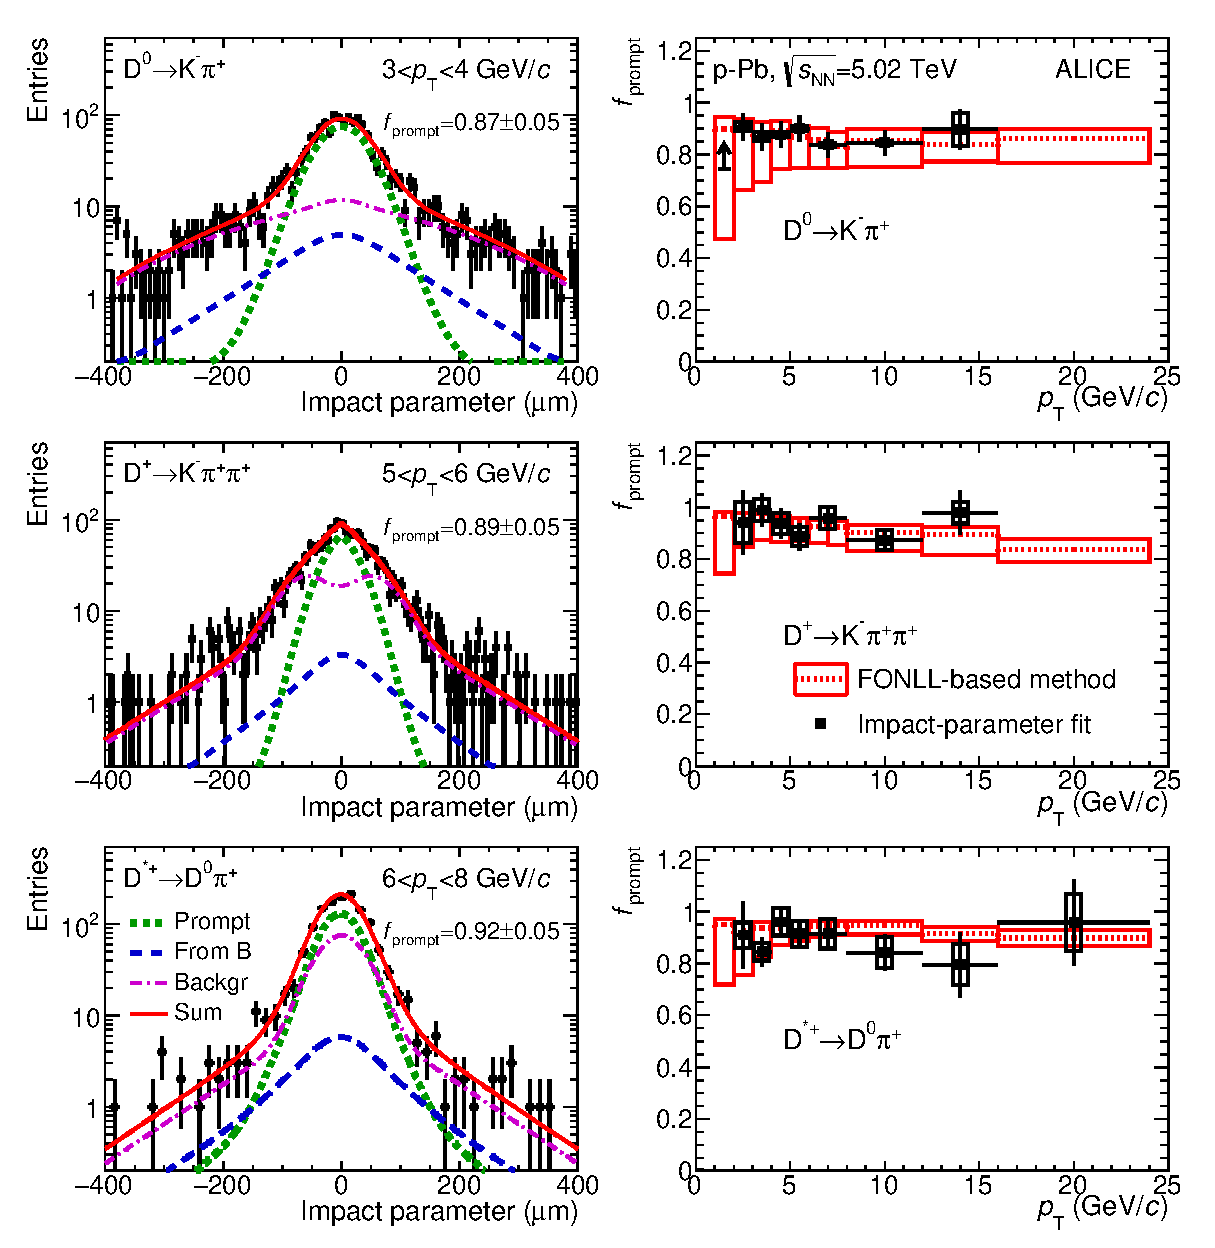
\includegraphics[scale=0.37]{ImpParFitAndRes.eps}}

\put(-5,91){
\begin{tikzpicture}[-]
\draw[draw=blue,solid,line width=0.3mm] (0, 0) -- + (7.6,0);
\end{tikzpicture}}

\put(-5,163){
\begin{tikzpicture}[-]
\draw[draw=blue,solid,line width=0.3mm] (0, 0) -- + (7.6,0);
\end{tikzpicture}}

\put(-5,91){
\begin{tikzpicture}[-]
\draw[draw=blue,solid,line width=0.3mm] (0, 0) -- + (0,2.54);
\end{tikzpicture}}

\put(211,91){
\begin{tikzpicture}[-]
\draw[draw=blue,solid,line width=0.3mm] (0, 0) -- + (0,2.54);
\end{tikzpicture}}

\put(211,215){\captionsetup{labelformat=empty}
\begin{minipage}[t]{0.38\linewidth}
\begin{itemize}
 \item La frazione di D$^+$ prompt misurata con il metodo del fit del parametro di impatto è compatibile con i metodi \textit{theory-driven}
 \item L'incertezza totale è compatibile con i metodi \textit{theory-driven} a $\pt$ intermedio e maggiore ad alto e basso $\pt$
 \item Risultato inserito come cross-check dei metodi theory-driven nell'articolo \textcolor{blue}{\textit{D-meson production in p-Pb collisions at $\sqrt{s_{NN}}=5.02$ TeV and in pp collisions at $\sqrt{s}=7$ TeV}} pubblicato dalla Collaborazione ALICE 
\end{itemize}
\end{minipage}}

\end{picture} 
\end{frame}

\section{Metodo della variazione dei tagli}
\begin{frame}
\frametitle{Metodo della variazione dei tagli}
\begin{picture}(320,250)

\put(10,115){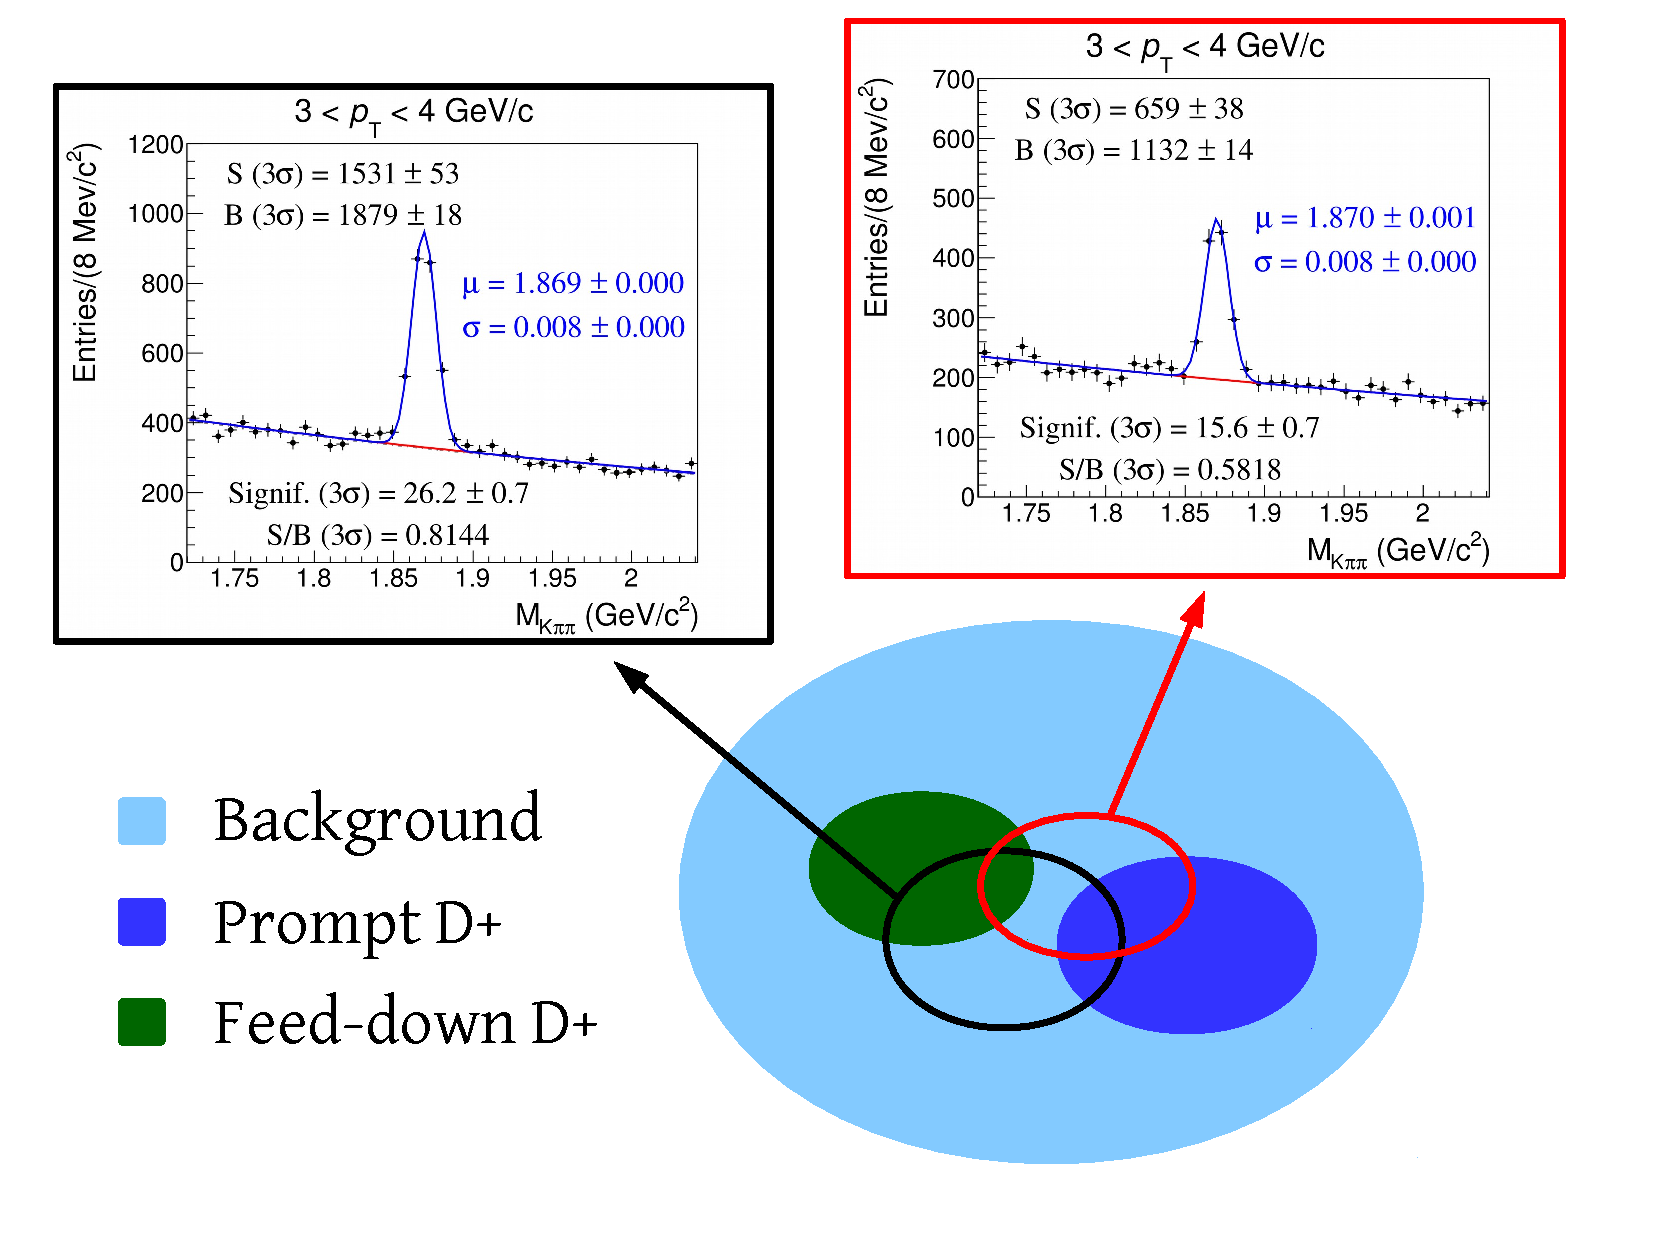
\includegraphics[scale=0.22]{cutvar_sketch.pdf}}

\put(195,245){\captionsetup{labelformat=empty}
\begin{minipage}[t]{0.4\linewidth}
\begin{center}
I candidati mesoni D$^+$ includono D$^+$ prompt, D$^+$ feed-down e il fondo combinatoriale \\[2mm]
Applicando selezioni su quantità topologiche per ottenere un buon rapporto segnale su fondo e una buona significatività statistica\\[-4mm] \[signif. = \frac{S}{\sqrt{S+B}},\] \\[-2mm]se ne seleziona soltanto una parte
\end{center}
\end{minipage}}

\put(0,110){\captionsetup{labelformat=empty}
\begin{minipage}[t]{0.55\linewidth}
\begin{center}
Per ogni set di tagli definito si ottiene un'equazione che ha come incognite il numero corretto di mesoni D$^+$ prompt e feed-down (\textcolor{blue}{$N_{prompt}$} e \textcolor{blue}{$N_{feed-down}$}) \\[2mm] $\Rightarrow$ per $n$ set di tagli si ottiene un sistema sovradeterminato
\end{center}
\end{minipage}}

\put(7,65){\captionsetup{labelformat=empty}
\begin{minipage}[t]{0.49\linewidth}
\begin{block}{}
\setlength\abovedisplayskip{0pt}
\begin{equation*}
\begin{cases}
\epsilon^{prompt}_1\cdot N_{prompt} + \epsilon^{feed-down}_1\cdot N_{feed-down} = Y_1\\
..\\
\epsilon^{prompt}_n\cdot N_{prompt} + \epsilon^{feed-down}_n\cdot N_{feed-down} = Y_n\\
\end{cases}
\label{cutvar_syst}
\end{equation*}
\end{block}
\end{minipage}}

\put(210,140){\captionsetup{labelformat=empty}
\begin{minipage}[t]{0.36\linewidth}
\begin{block}{}
\setlength\abovedisplayskip{0pt}
\begin{itemize}
\item \textcolor{blue}{Raw yield $Y$}: numero grezzo di D$^+$ estratto dal fit di massa invariante
\item \textcolor{blue}{Efficienza $\epsilon_X$}: rapporto tra numero di D$^+$ prompt (feed-down) ricostruite e generate 
\item \textcolor{blue}{Corrected yield $N_X$}: numero di D$^+$ prompt (feed-down) corretto per l'efficienza
\end{itemize}
\end{block}
\end{minipage}}

\end{picture}
\end{frame}

\begin{frame}
\frametitle{Metodi di minimizzazione}
\begin{picture}(320,250)

\put(-5,5){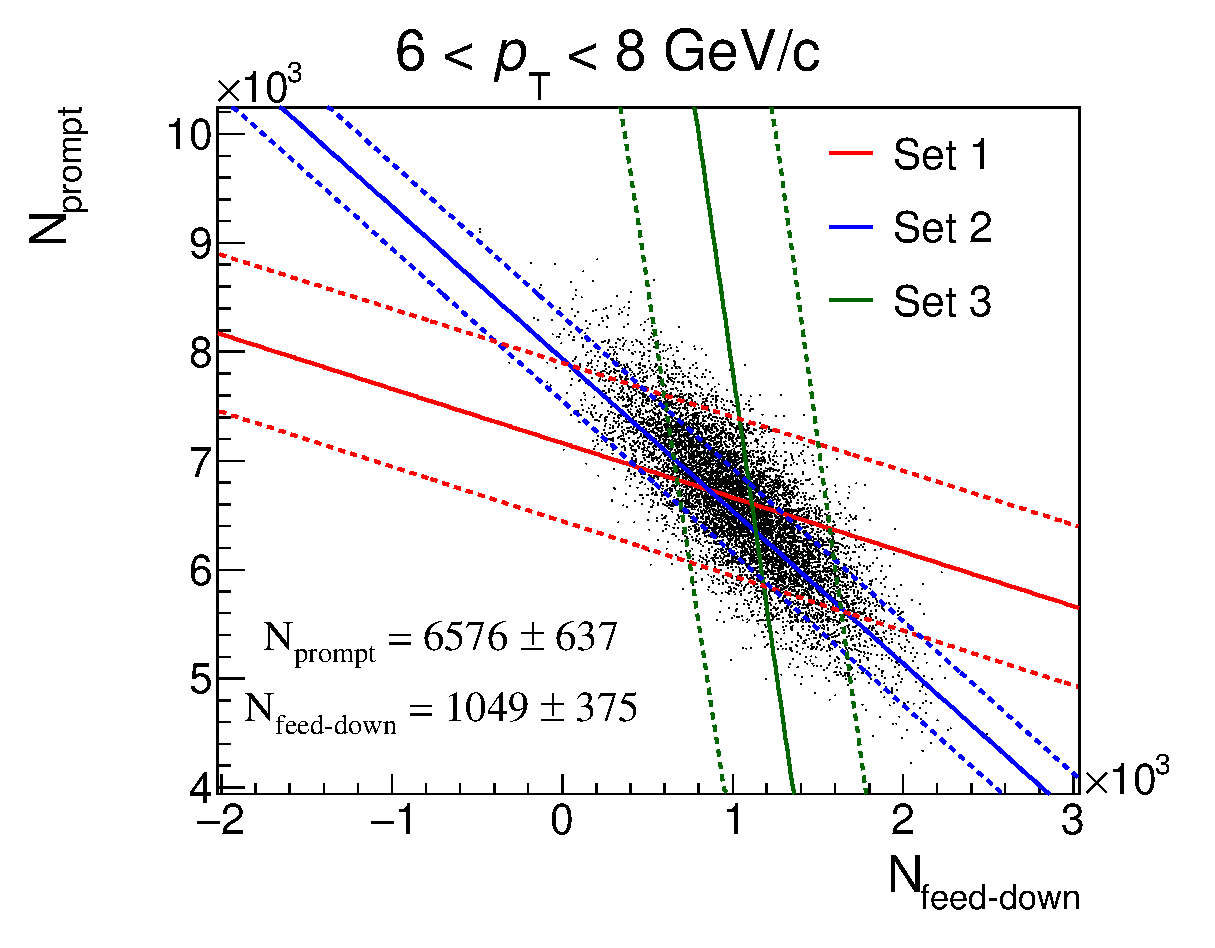
\includegraphics[scale=0.24]{LinesDisp_6-8.eps}}

\put(0,234){\captionsetup{labelformat=empty}
\begin{minipage}[t]{0.7\linewidth}
\begin{equation*}
\renewcommand\arraystretch{1.3} {
\left(
\begin{array}{cc}
\epsilon^{prompt}_1 & \epsilon^{feed-down}_1\\
\epsilon^{prompt}_2 & \epsilon^{feed-down}_2\\
.. & ..\\
\epsilon^{prompt}_n & \epsilon^{feed-down}_n
\end{array}
 \right)} 
 \times
 \left(
\begin{array}{c}
 N_{prompt}\\
 N_{feed-down}
\end{array}
 \right) 
 -
  \left(
\begin{array}{c}
Y_1\\
Y_2\\
..\\
Y_n
\end{array}
 \right)
 = \textcolor{red}{
\left(
\begin{array}{c}
\delta_1\\
\delta_2\\
..\\
\delta_n
\end{array}
 \right)}
\end{equation*} 
\end{minipage}}

\put(250,220){\captionsetup{labelformat=empty}
\begin{minipage}[t]{0.25\linewidth}
\begin{center}
Il vettore nullo è sostituito dal vettore dei residui $\pmb{\textcolor{red}{\delta}}$
\end{center}
\end{minipage}}

\put(0,160){\captionsetup{labelformat=empty}
\begin{minipage}[t]{0.6\linewidth}
Il numero corretto di mesoni D$^+$ prompt e feed-down e la matrice delle covarianze associata sono ottenuti dalla minimizzazione del $\chi^2 = \pmb{\delta}^T \pmb{C}^{-1} \pmb{\delta}$ 
\end{minipage}}

\put(180,175){\captionsetup{labelformat=empty}
\begin{minipage}[t]{0.6\linewidth}
\[
\pmb{C} = 
\left(
\begin{array}{cccc}
\sigma^2_{\delta_1} & & &\\
 & \sigma^2_{\delta_2} & &\\
 & & \ddots &\\
 &  &  & \sigma^2_{\delta_n}
\end{array}
 \right) 
\]
\end{minipage}}

\put(0,240){\captionsetup{labelformat=empty}
\begin{minipage}[t]{0.5\linewidth}
\begin{itemize}
 \item \textcolor{blue}{Minimizzazione analitica} \\[3.7cm]
 \item \textcolor{blue}{Determinazione dell'incentro}
\end{itemize}
\end{minipage}}

\put(135,95){\captionsetup{labelformat=empty}
\begin{minipage}[t]{0.6\linewidth}
Ogni equazione corrispondente ad un set di tagli descrive una retta nel piano $(N_{prompt}, N_{feed-down})$\\ $\Rightarrow$ le intersezioni di tre rette definiscono un triangolo \\$\Rightarrow$ $N_{prompt}$ e $N_{feed-down}$ sono determinati dalle coordinate dell'incentro del triangolo \\[2mm]
L'errore statistico è valutato con una simulazione Monte Carlo, in cui i parametri delle rette sono estratti da distribuzioni Gaussiane 
\end{minipage}}

\end{picture}
\end{frame}

\begin{frame}
\frametitle{Strategia per la scelta dei set di tagli}
\begin{picture}(320,250)

\put(-5,15){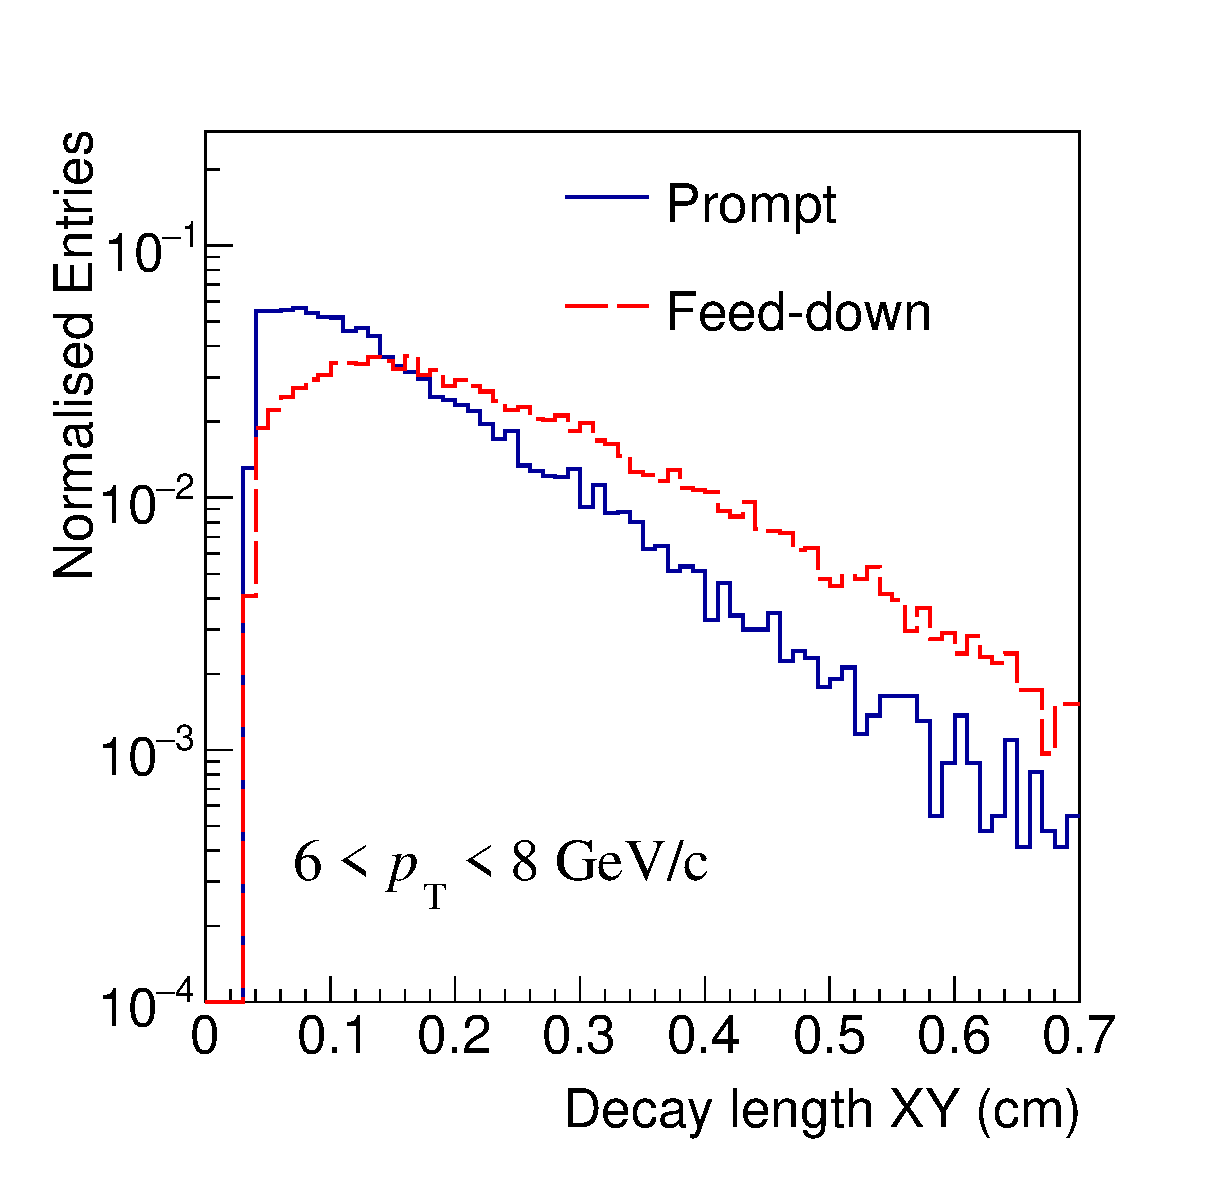
\includegraphics[scale=0.16]{CompPromptFD_DLXY_6-8.eps}}
\put(83,15){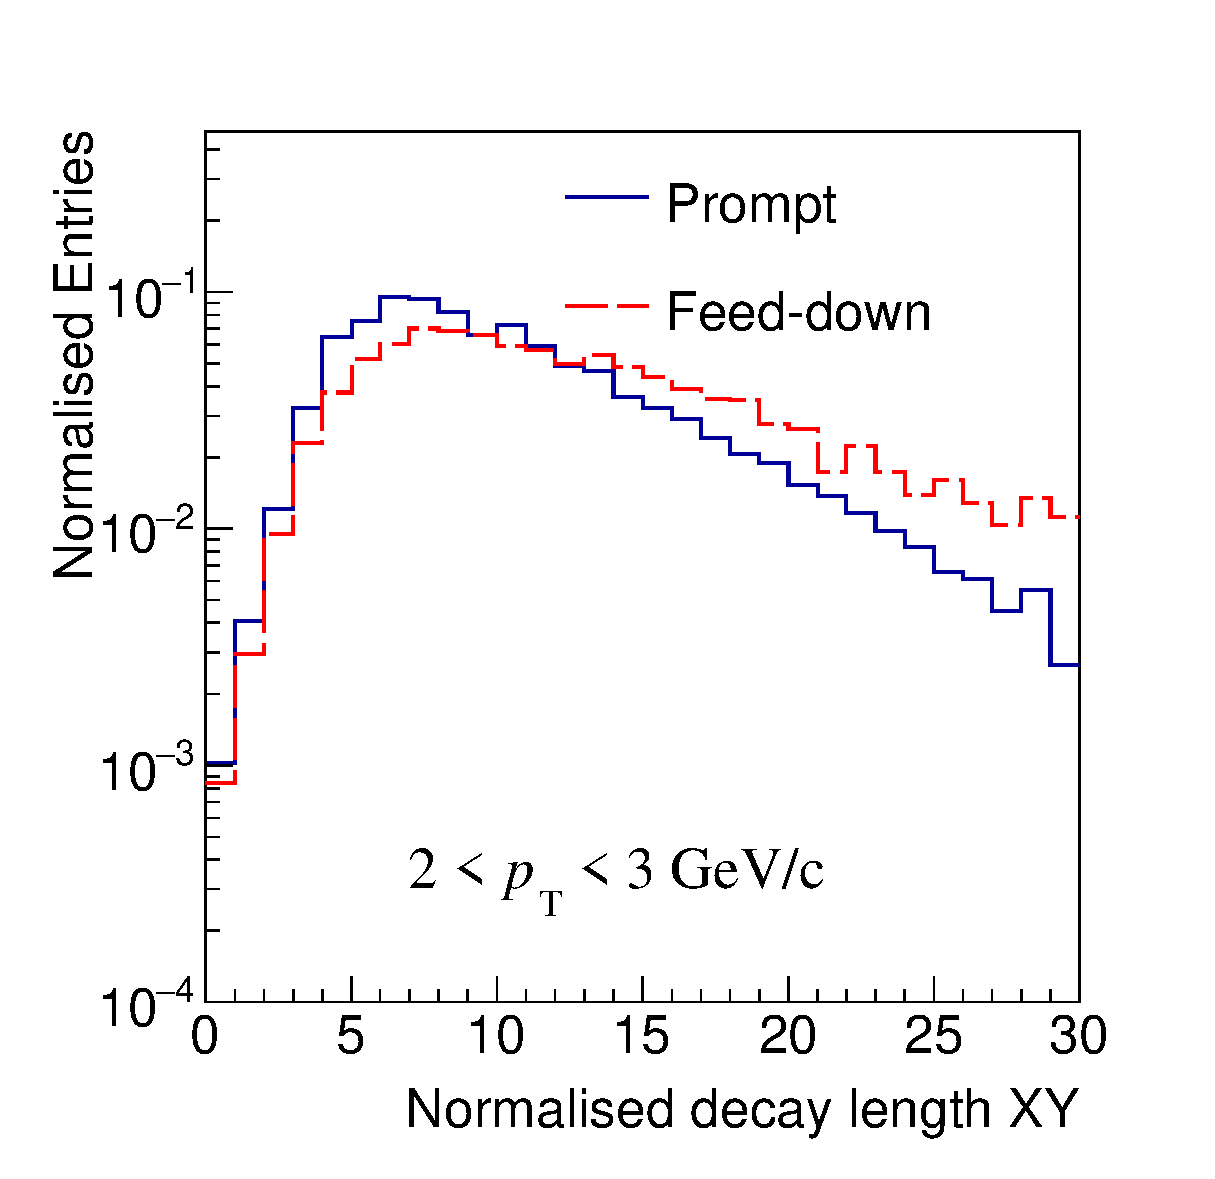
\includegraphics[scale=0.16]{CompPromptFD_NDLXY_2-3.eps}}
\put(176,15){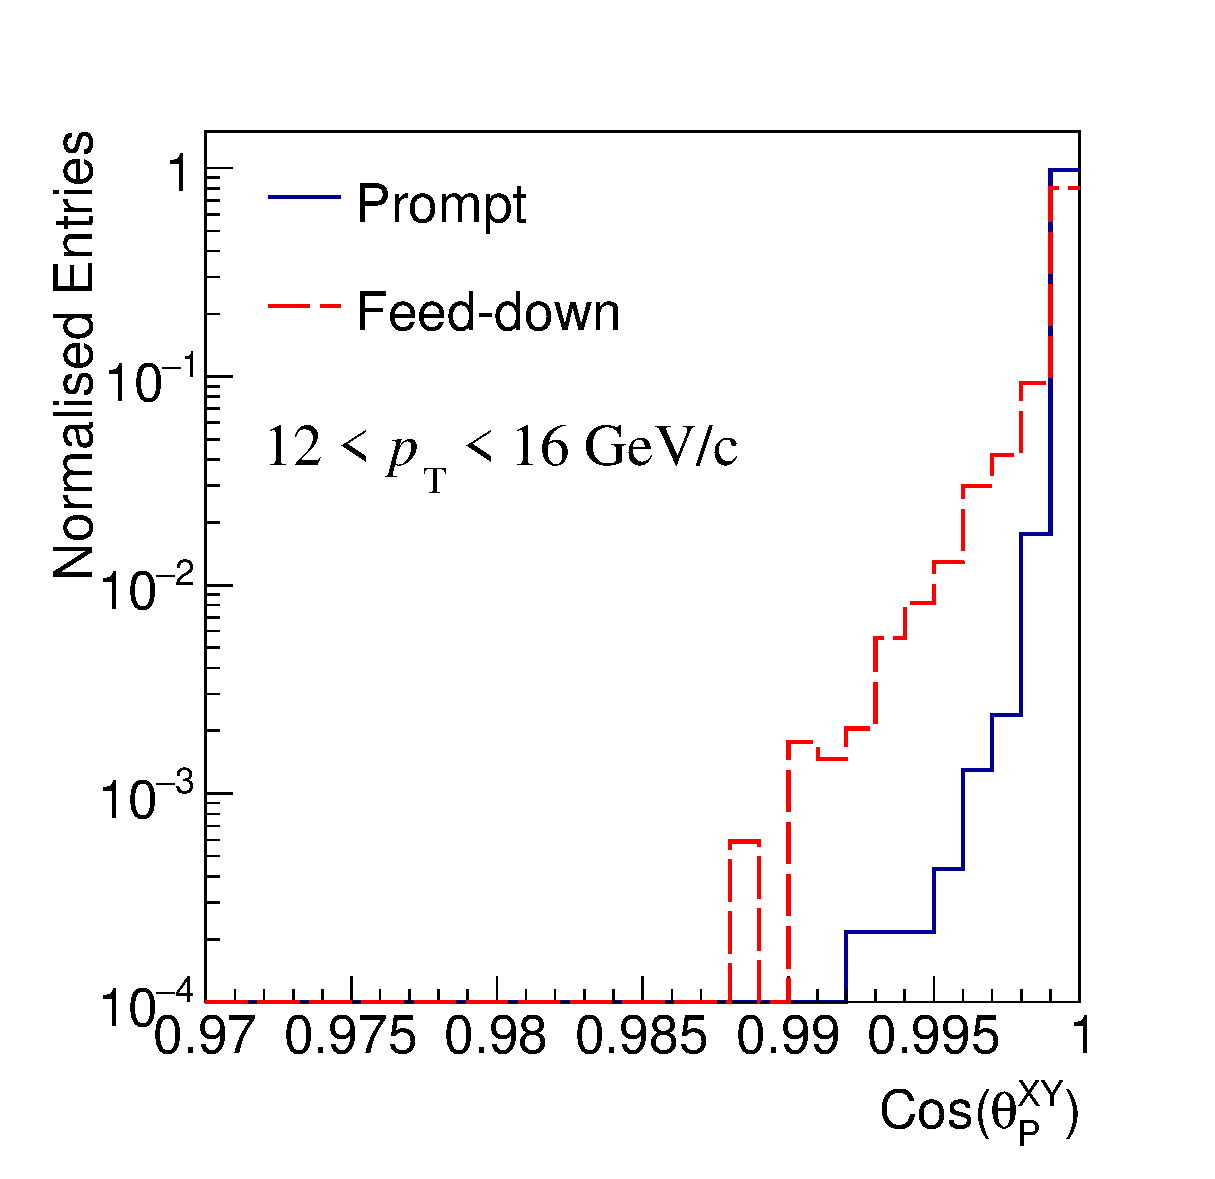
\includegraphics[scale=0.16]{CompPromptFD_CospXY_12-16.eps}}
\put(264,15){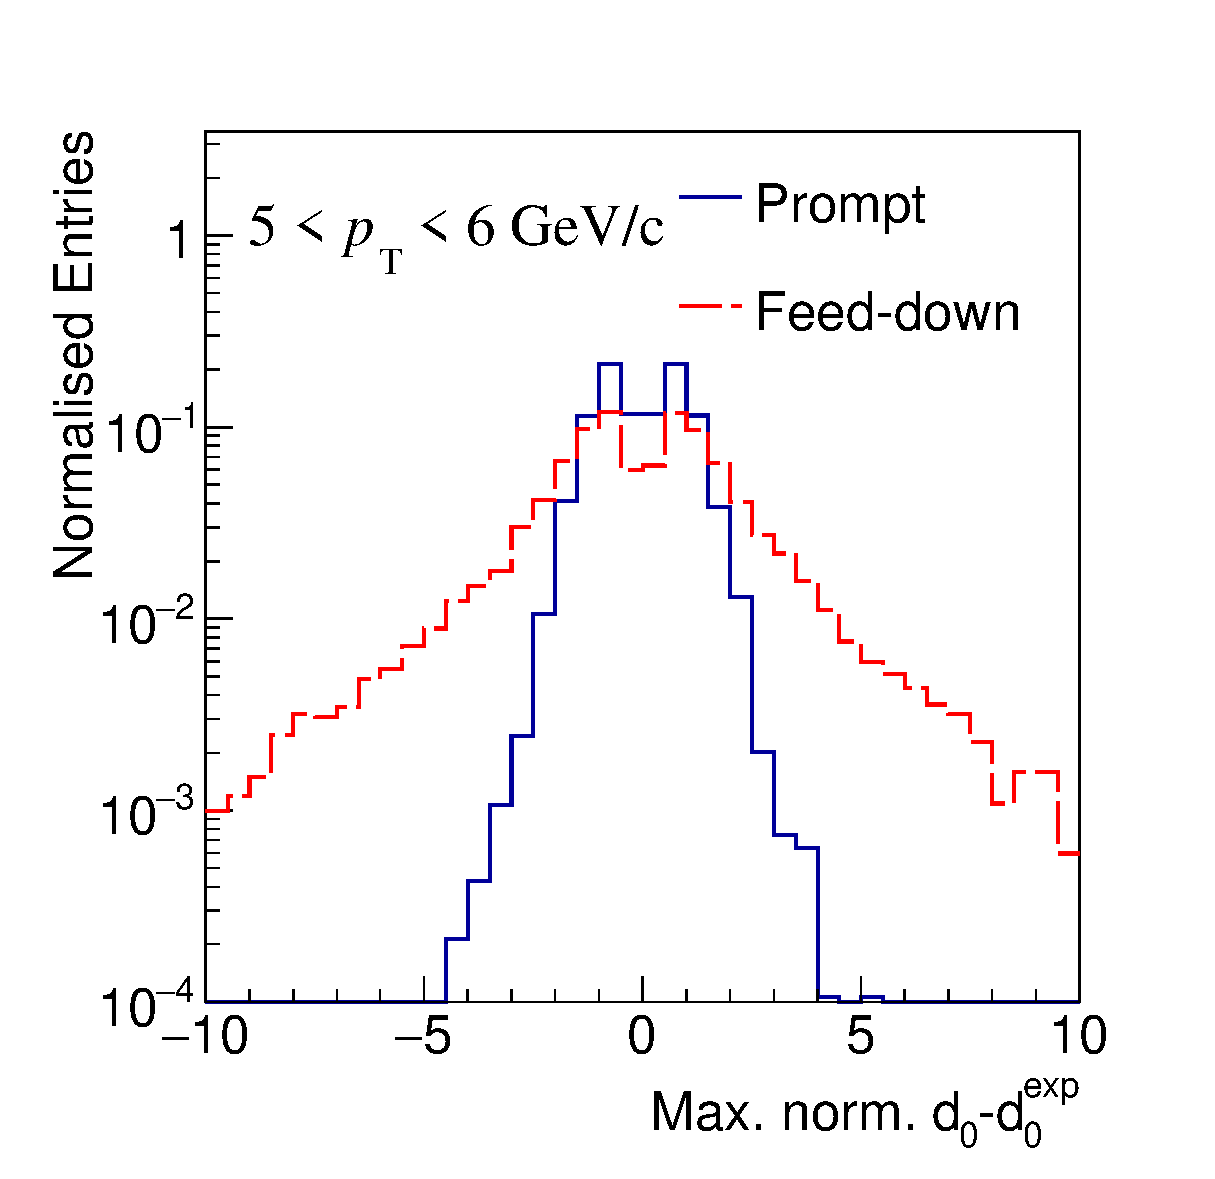
\includegraphics[scale=0.16]{CompPromptFD_d0d0exp_5-6.eps}}

\put(0,235){\captionsetup{labelformat=empty}
\begin{minipage}[t]{1.\linewidth}
Sono stati utilizzati tre set di tagli il più possibile \textcolor{blue}{scorrelati}:\\[2.3cm]
Variabili topologiche usate per definire i set di tagli:
\end{minipage}}

\put(25,231){
\begin{minipage}[t]{0.85\linewidth}
\begin{block}{}
\setlength\abovedisplayskip{0pt}
\begin{itemize}
 \item 1$^o$ set: aumento dell'efficienza di selezione dei mesoni D$^+$ prompt 
 \item 2$^o$ set: intermedio (buon estrazione del segnale)
 \item 3$^o$ set: aumento dell'efficienza di selezione dei mesoni D$^+$ feed-down
\end{itemize}
\end{block}
\end{minipage}}

\put(0,145){
\begin{minipage}[t]{0.25\linewidth}
\begin{itemize}
 \item Lunghezza di decadimento nel piano trasverso
\end{itemize}
\end{minipage}}

\put(85,145){
\begin{minipage}[t]{0.25\linewidth}
\begin{itemize}
 \item Lunghezza di decadimento nel piano trasverso normalizzata al proprio errore
\end{itemize}
\end{minipage}}

\put(175,145){
\begin{minipage}[t]{0.25\linewidth}
\begin{itemize}
 \item Coseno dell'\\angolo di \\pointing nel \\piano trasverso
\end{itemize}
\end{minipage}}

\put(260,155){
\begin{minipage}[t]{0.25\linewidth}
\begin{itemize}
 \item Massima differenza normalizzata tra il parametro di impatto atteso e misurato delle tracce figlie
\end{itemize}
\end{minipage}}

\end{picture}
\end{frame}

\begin{frame}
\frametitle{Metodo della variazione dei tagli\\ Risultato}
\begin{picture}(320,250)

\put(-5,88){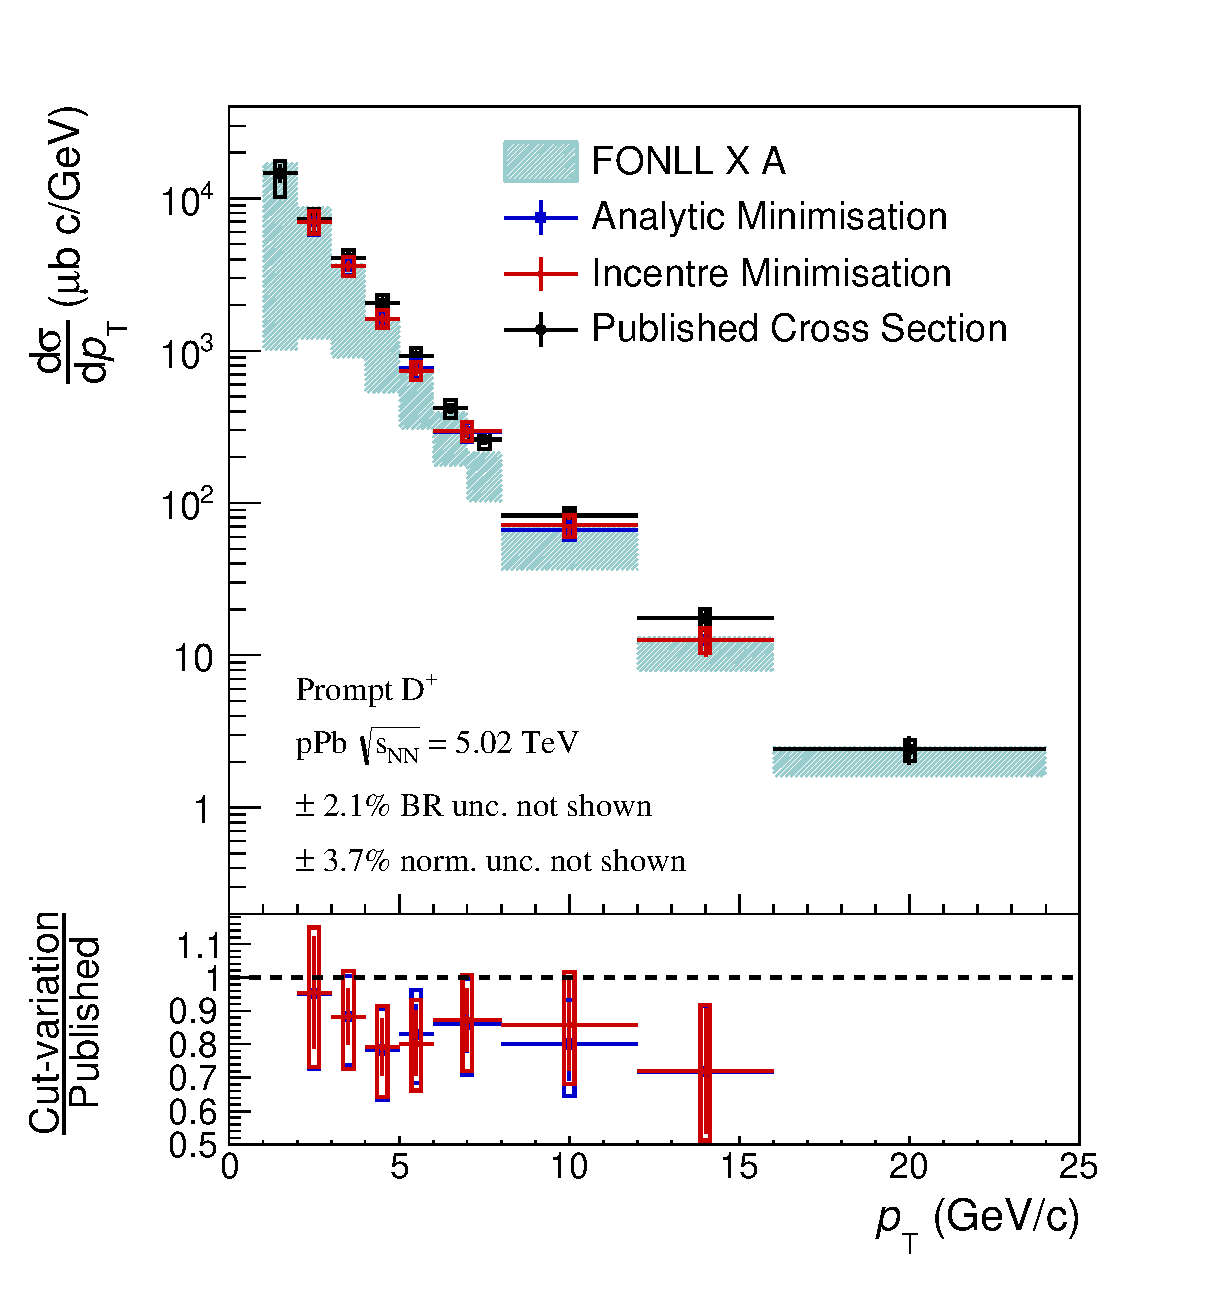
\includegraphics[scale=0.25]{CrossSectionPromptpPb.eps}}
\put(130,91){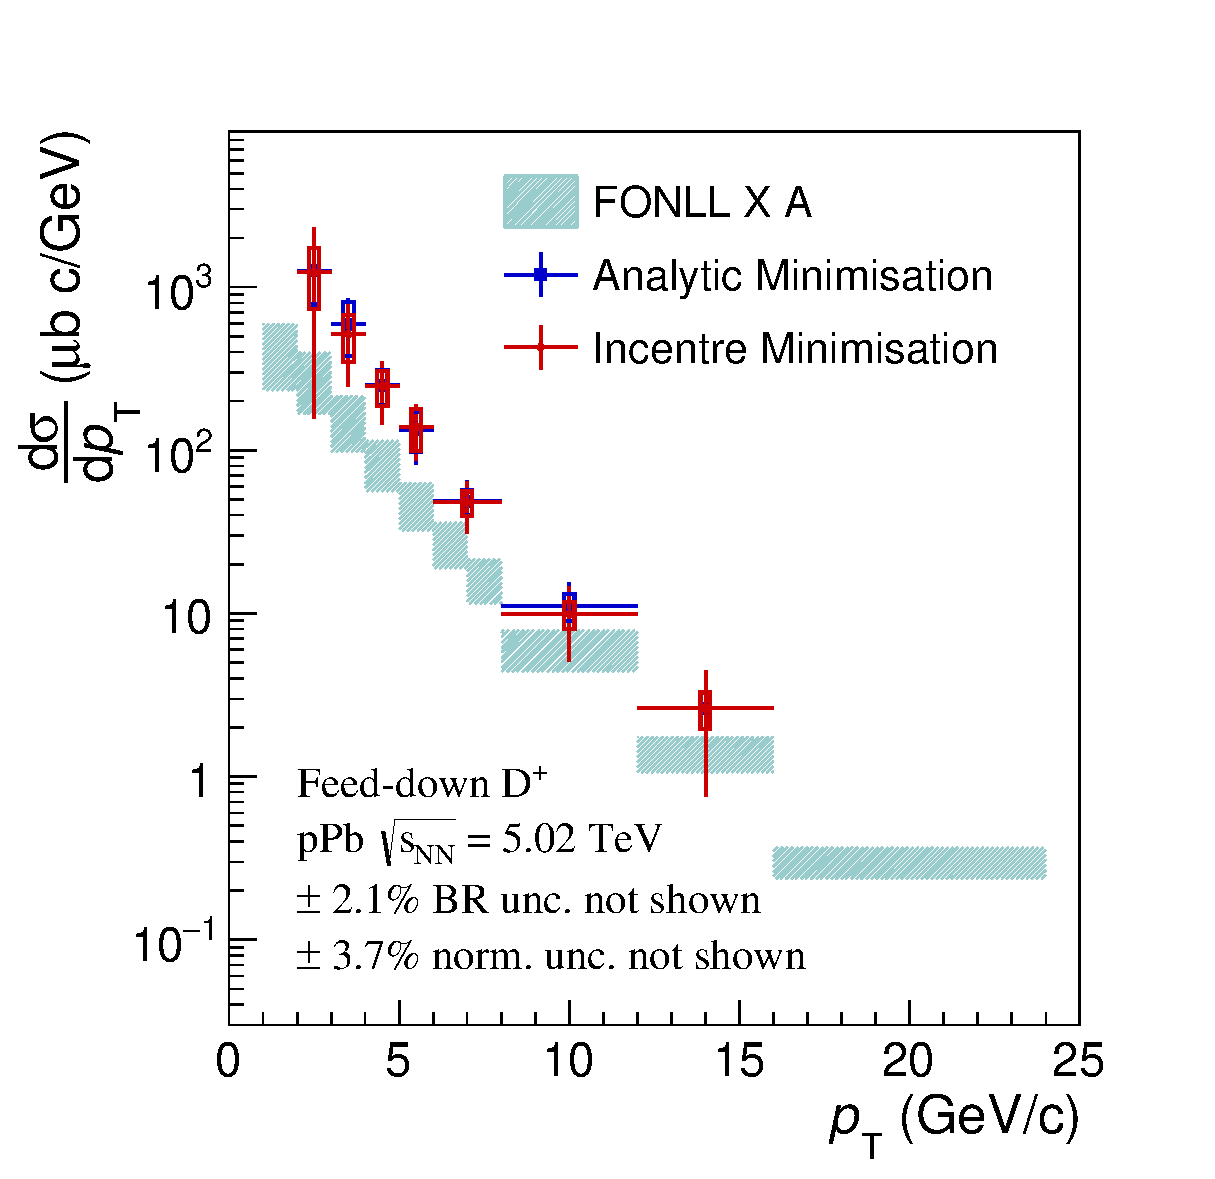
\includegraphics[scale=0.24]{CrossSectionFDpPb.eps}}

\put(175,280){\captionsetup{labelformat=empty}
\begin{minipage}[t]{0.45\linewidth}
\begin{block}{}
\setlength\abovedisplayskip{0pt}
\begin{equation*}
\frac{d\sigma^{D^+}_X}{d\pt}\bigg{|}_{|y|<0.5} = \frac{1}{2}\cdot \frac{N^{D^\pm}_X|_{|y|<y_{fid}}}{\Delta \pt \Delta y \cdot(Acc)_X} \cdot\frac{L_{int}}{BR}
\end{equation*}
\end{block} 
\end{minipage}}

\put(258,210){\captionsetup{labelformat=empty}
\begin{minipage}[t]{0.25\linewidth}
Sorgenti di errore \\sistematico:
\begin{itemize}
 \item Estrazione del segnale 
 \item Efficienza di selezione dei tagli topologici
 \item Imperfetta descrizione delle distribuzioni di $\pt$ \\di mesoni D$^+$ e B generati nella simulazione \\Monte Carlo
\end{itemize}
\end{minipage}}

\put(20,235){\captionsetup{labelformat=empty}
\begin{minipage}[t]{0.25\linewidth}
\textcolor{blue}{D$^+$ prompt}
\end{minipage}}

\put(155,213){\captionsetup{labelformat=empty}
\begin{minipage}[t]{0.25\linewidth}
\textcolor{blue}{D$^+$ feed-down}
\end{minipage}}

\put(-5,85){\captionsetup{labelformat=empty}
\begin{minipage}[t]{0.85\linewidth}
\begin{itemize}
 \item Sezione d'urto differenziale in $\pt$ di produzione dei mesoni D$^+$\\ prompt $\Rightarrow$ compatibile con il risultato pubblicato e la predizione di \\FONLL 
 \item Sezione d'urto differenziale in $\pt$ di produzione dei mesoni D$^+$ feed-down \\$\Rightarrow$ sistematicamente maggiore rispetto alla predizione di FONLL  
\end{itemize}
\end{minipage}}

\end{picture}
\end{frame}

\section{Metodo di ricostruzione dei mesoni D$^+$ con il filtro di Kalman}
\begin{frame}
\frametitle{Metodo di ricostruzione dei mesoni D$^+$ con il filtro di Kalman}
\begin{picture}(320,250)

\put(135,15){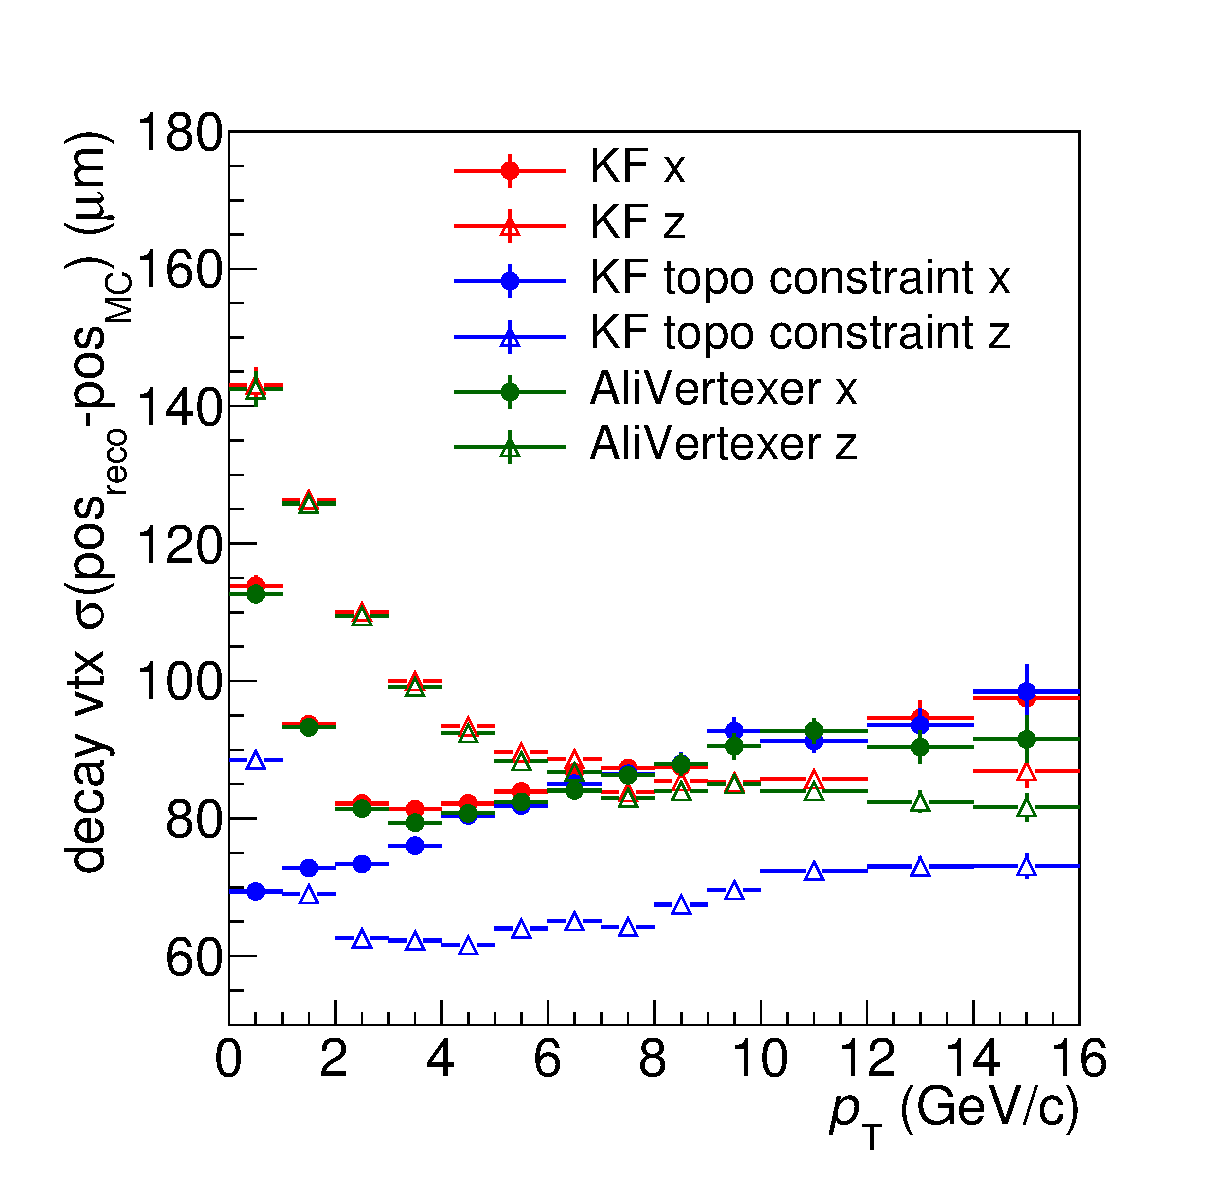
\includegraphics[scale=0.18]{ResSVXZ.eps}}
\put(240,15){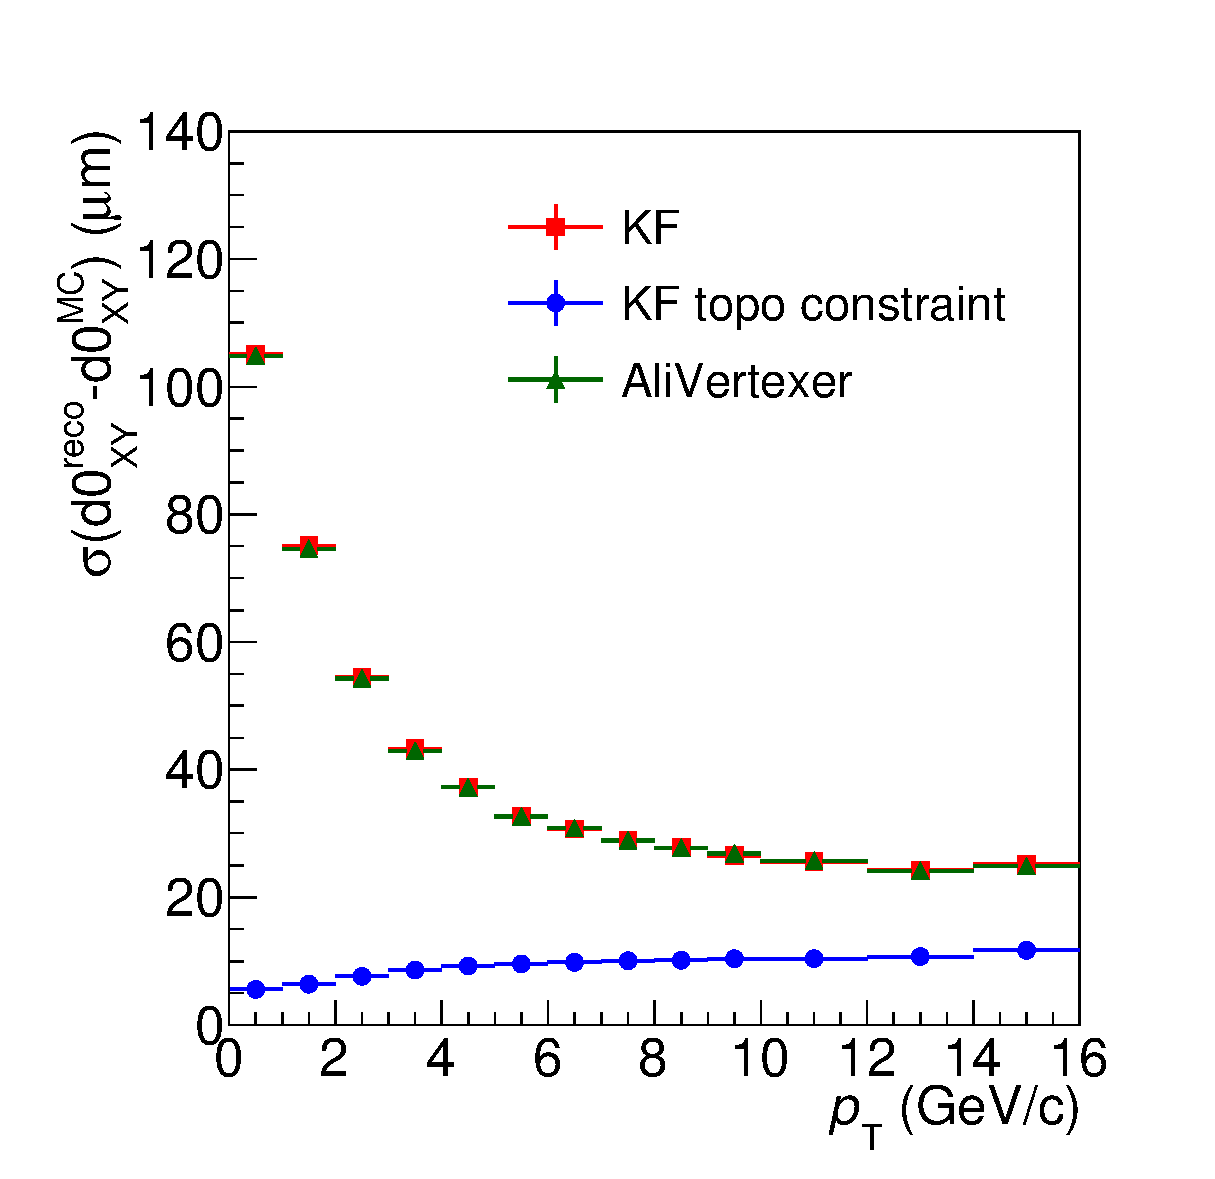
\includegraphics[scale=0.18]{ResImpPar.eps}}

\put(10,245){\captionsetup{labelformat=empty}
\begin{minipage}[t]{0.5\linewidth}
\begin{block}{\centering Filtro di Kalman}
\begin{center}
Algoritmo che permette di stimare un vettore di stato $\pmb{r}$ e la sua matrice delle covarianze $\pmb{C}$ a partire da $n$ misure $\pmb{m}_k$ ($k=1,..,n$) contenenti rumore statistico
\end{center}
\end{block} 
\end{minipage}}

\put(230,245){\captionsetup{labelformat=empty}
\begin{minipage}[t]{0.3\linewidth}
\begin{block}{\centering KFParticle package}
\begin{center}
Pacchetto per la ricostruzione di vertici di decadimento sviluppato per l'esperimento CBM basato sul filtro di Kalman \\$\Downarrow$\\ vettore di stato:\\ $\pmb{r} = (x,y,z,p_x,p_y,p_z,E,s)$
\end{center}
\end{block} 
\end{minipage}}

\put(195,205){
\begin{tikzpicture}[->]
\draw[draw=blue,solid,line width=0.3mm] (0, 0) -- + (0.8,0);
\end{tikzpicture}}

\put(0,160){\captionsetup{labelformat=empty}
\begin{minipage}[t]{0.8\linewidth}
\textcolor{blue}{Vantaggi del KFParticle package}:
\begin{itemize}
\item Valutazione del vettore di stato e della \\matrice di covarianza lungo la traiettoria \\della particella valutata con il filtro di Kalman
\item Possibilità di fissare dei vincoli $\Rightarrow$ \textit{mass constraint, \textcolor{blue}{topological constraint}}
\end{itemize}
\end{minipage}}

\put(0,85){\captionsetup{labelformat=empty}
\begin{minipage}[t]{0.35\linewidth}
Test delle performance eseguito sulla simulazione Monte Carlo selezionando i mesoni D$^+$ \textcolor{blue}{prompt}\\
$\Rightarrow$ risoluzione della variabile $X$:\\
\[Res(\pt) = \sigma(X_{reco}-X_{MC}) (\pt)\]
\end{minipage}}

\end{picture}
\end{frame}

\begin{frame}
\frametitle{Distribuzioni di $\chi^2/ndf$ dopo l'applicazione del \textit{topological constraint}}
\begin{picture}(320,250)

\put(0,235){\captionsetup{labelformat=empty}
\begin{minipage}[t]{0.95\linewidth}
I mesoni D$^+$ feed-down  \textcolor{blue}{non} derivano dal vertice primario di interazione dei fasci \\[1mm]
$\Rightarrow$ L'applicazione del \textcolor{blue}{topological constraint} al vertice primario permette di ridurre il contributo di mesoni D$^+$ da B, valutando il \textcolor{blue}{$\chi^2$} del vettore di stato dei candidati mesoni D$^+$
\end{minipage}}

\put(35,78){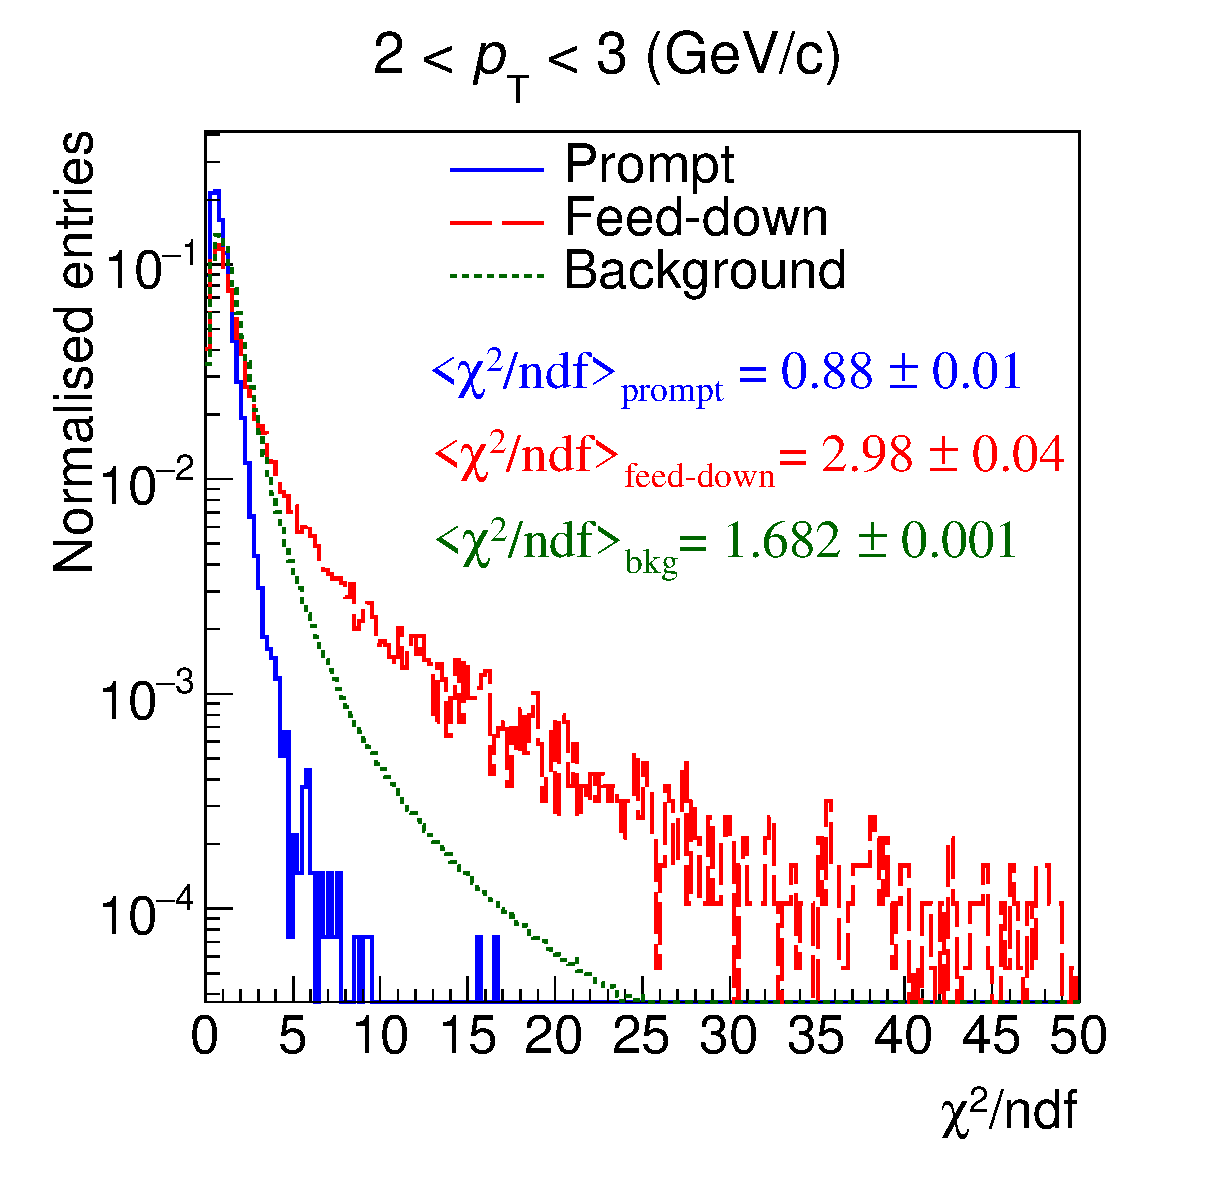
\includegraphics[scale=0.22]{KFchi_Dplus_pT1.eps}}
\put(180,78){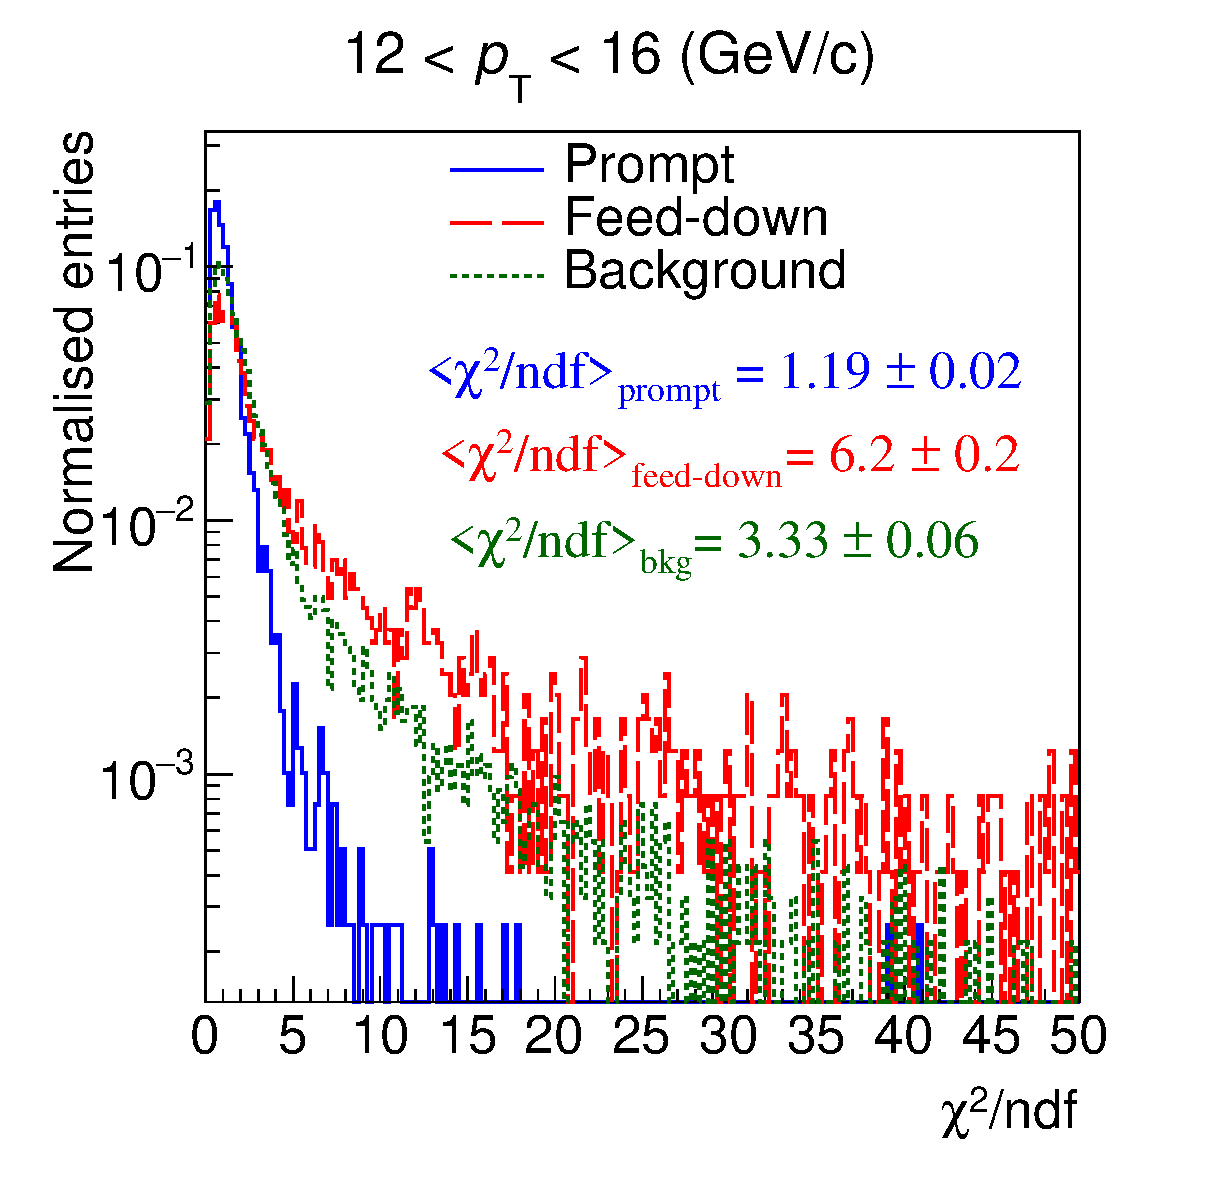
\includegraphics[scale=0.22]{KFchi_Dplus_pT8.eps}}

\put(5,66){\captionsetup{labelformat=empty}
\begin{minipage}[t]{0.95\linewidth}
$\Rightarrow$ selezione su $\chi^2/ndf$ dei candidati mesoni D$^+$, oltre alle selezioni sulle quantità topologiche usate nell'analisi standard 
\end{minipage}}

\put(210,55){\captionsetup{labelformat=empty}
\begin{minipage}[t]{0.35\linewidth}
\begin{block}{}
\centering
set centrale ottimizzato variando la selezione tra $[-1.5,1.5]$
\end{block}
\end{minipage}}

\put(10,30){\captionsetup{labelformat=empty}
\begin{minipage}[t]{0.9\linewidth}
\renewcommand\arraystretch{1.4} 
  \begin{tabular}{c|c|c|c|c}
    $\pt$ (GeV/c) & $[1,2]$ & $[2,8]$ & $[8,16]$ & $[16,24]$ \\
    \hline
    $\chi^2/ndf$ & $<2.5$ & $<3.0$ & $<3.5$ & $<4.0$ \\
    \end{tabular}
\end{minipage}}

\end{picture}
\end{frame}

\begin{frame}
\frametitle{Studio della variazione della selezione su $\chi^2/ndf$}
\begin{picture}(320,250)

\put(10,15){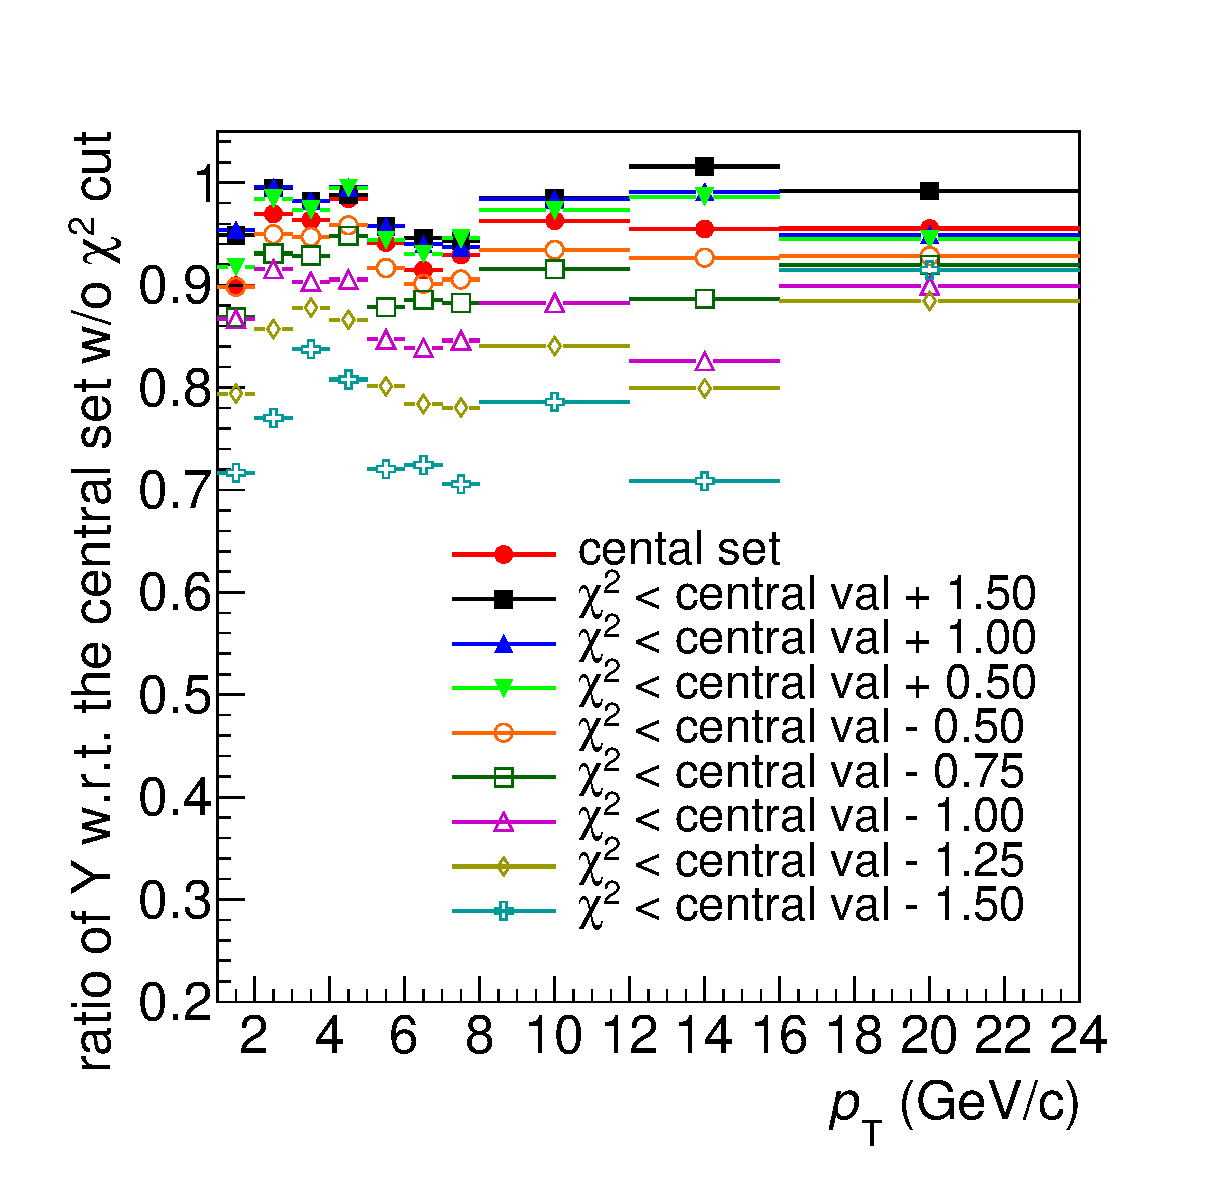
\includegraphics[scale=0.2]{KF_CutVarSyst_ratioraw_chiS.eps}}
\put(130,130){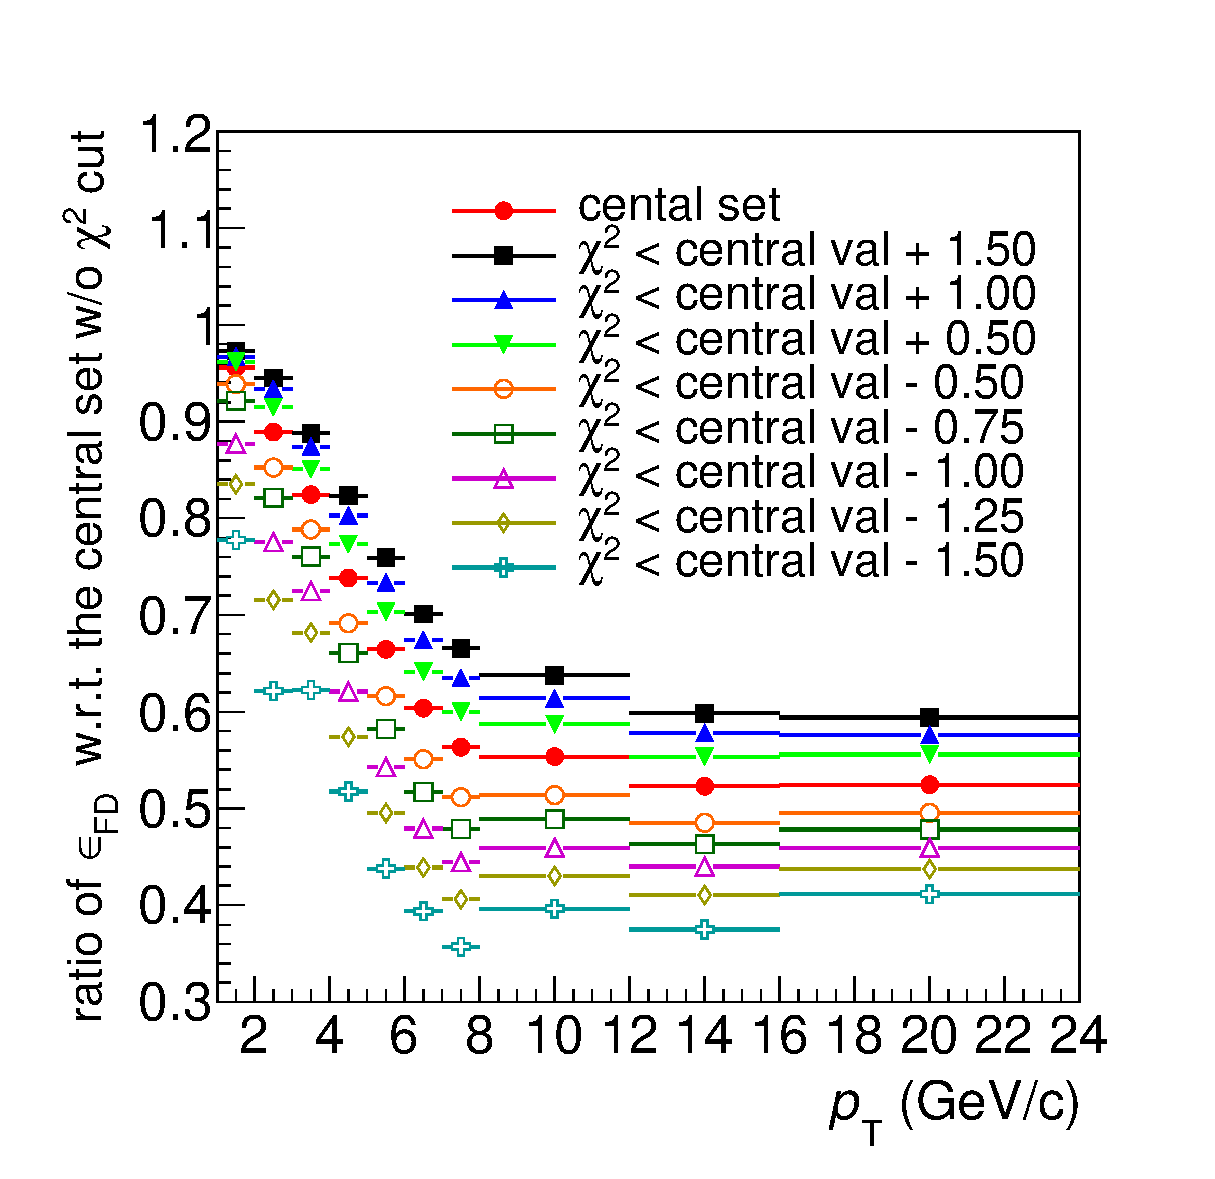
\includegraphics[scale=0.2]{KF_CutVarSyst_ratioeffFD_chiS.eps}}
\put(10,130){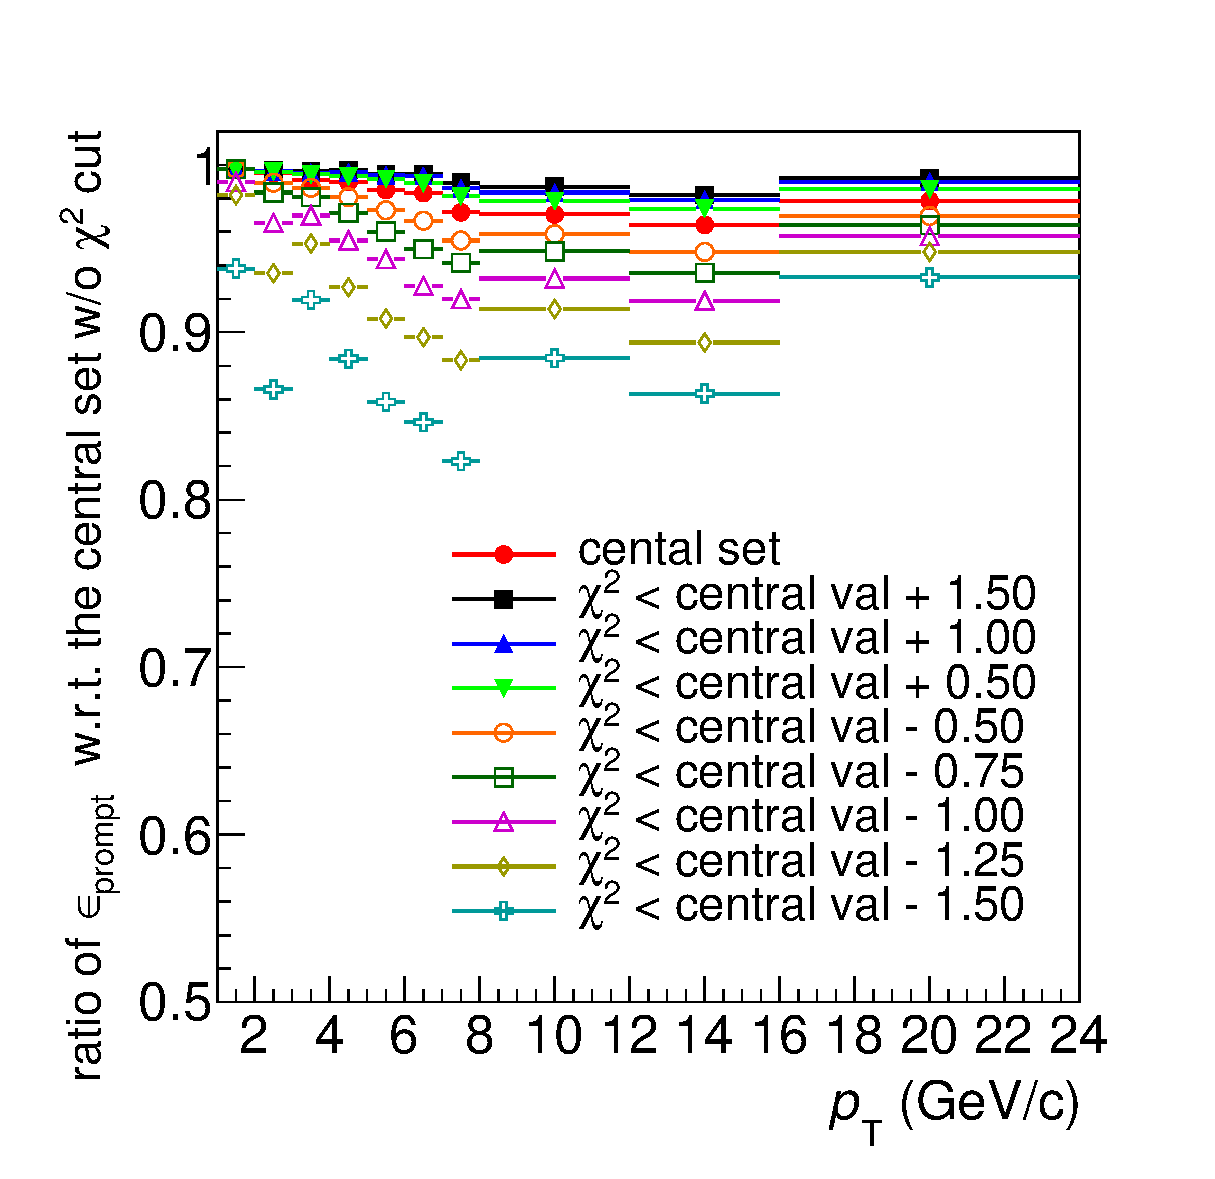
\includegraphics[scale=0.2]{KF_CutVarSyst_ratioeffprompt_chiS.eps}}
\put(130,15){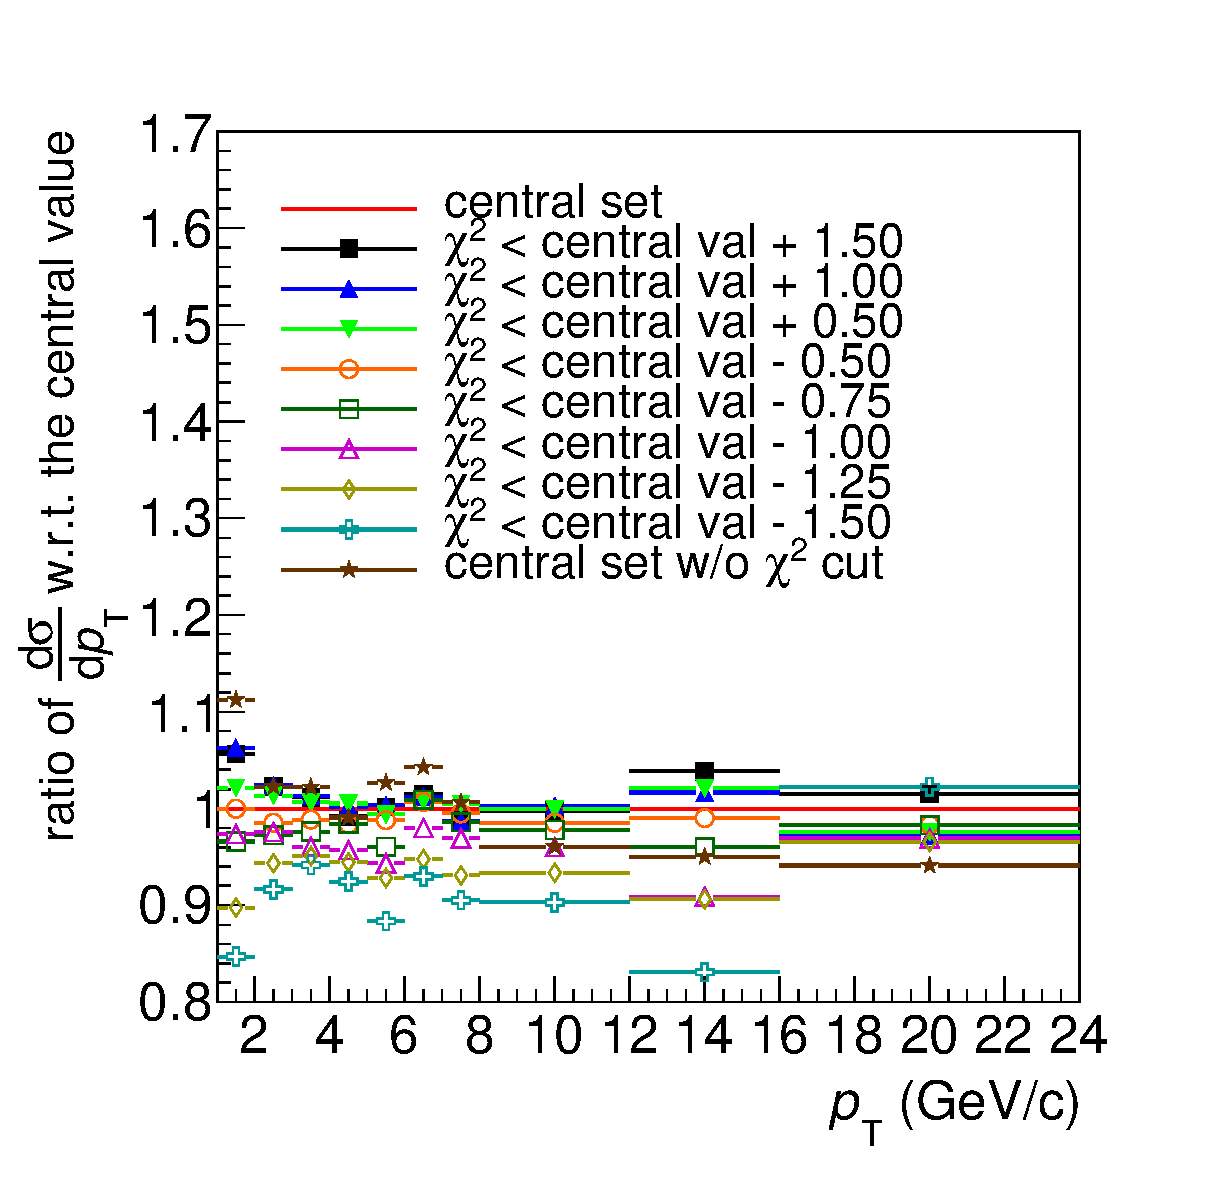
\includegraphics[scale=0.2]{KF_CutVarSyst_ratioonly_chiS.eps}}

\put(238,215){\captionsetup{labelformat=empty}
\begin{minipage}[t]{0.3\linewidth}
\begin{itemize}
 \item La riduzione dell'efficienza ottenuta applicando una selezione su $\chi^2/ndf$ raggiunge il \textcolor{blue}{20\%} per i mesoni D$^+$ \textcolor{blue}{prompt} e il \textcolor{red}{60\%} per i mesoni D$^+$ \textcolor{red}{feed-down} 
\item La perdita di segnale non supera il 30\%
\item Applicando una selezione molto ``stretta'' su $\chi^2/ndf$ si osserva una riduzione sistematica della sezione d'urto differenziale  
\end{itemize}
\end{minipage}}

\end{picture}
\end{frame}

\begin{frame}
\frametitle{Metodo di ricostruzione dei mesoni \\D$^+$ con il filtro di Kalman - Risultato}
\begin{picture}(320,250)

\put(10,150){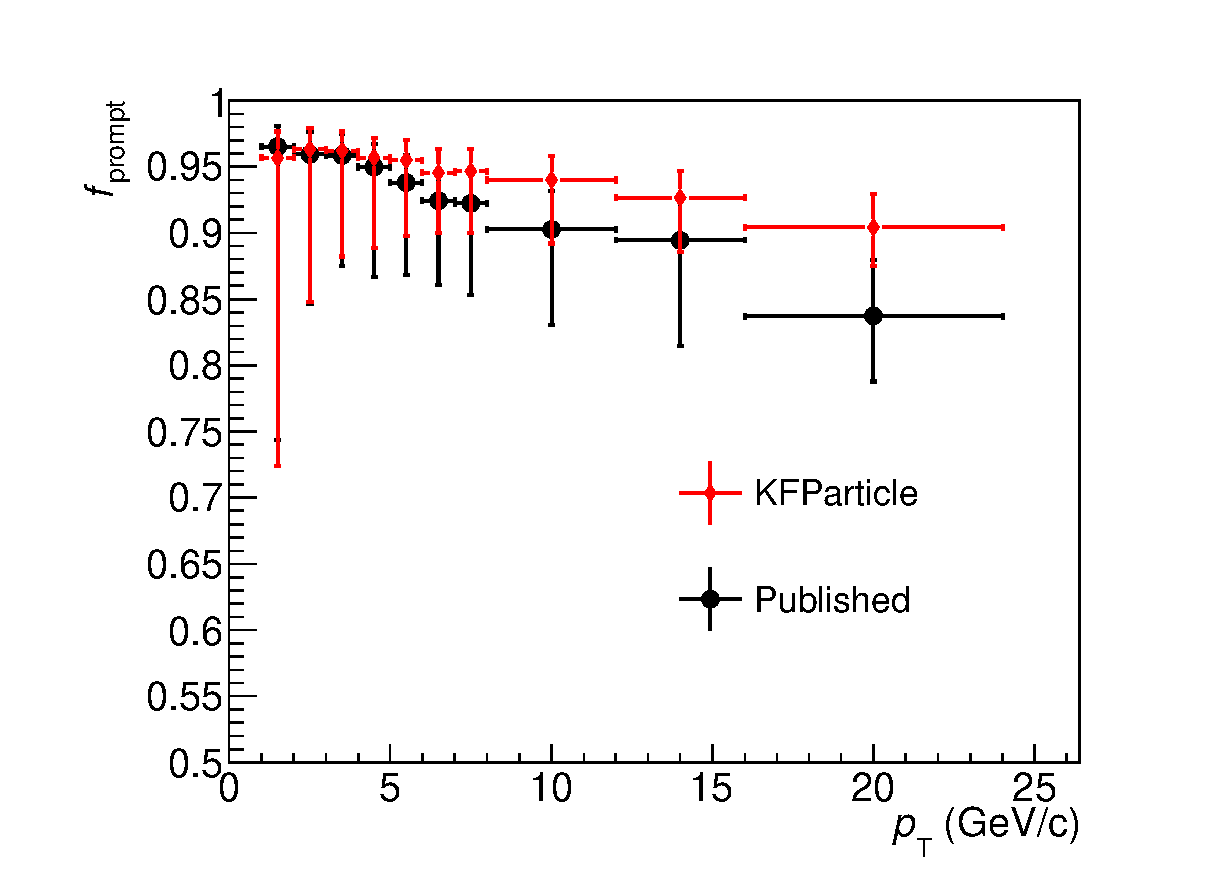
\includegraphics[scale=0.24]{PromptFrac_KF.eps}}
\put(175,70){\includegraphics[scale=0.26]{CrossSection_KF.eps}}

\put(185,275){\captionsetup{labelformat=empty}
\begin{minipage}[t]{0.45\linewidth}
\begin{block}{}
\fontsize{6.5}{10}\selectfont
\setlength\abovedisplayskip{0pt}
\begin{equation*}
\frac{d\sigma^{D^+}_{prompt}}{d\pt}\bigg{|}_{|y|<0.5} = \frac{1}{2}\cdot \frac{f_{prompt}\cdot N^{D^\pm}_{raw}|_{|y|<y_{fid}}}{\Delta \pt \Delta y \cdot(Acc\times\epsilon)_{prompt}} \cdot\frac{L_{int}}{BR}
\end{equation*}
\end{block} 
\end{minipage}}


\put(0,140){\captionsetup{labelformat=empty}
\begin{minipage}[t]{1.\linewidth}
\begin{itemize}
 \item La frazione di D$^+$ prompt è maggiore \\rispetto a quella ottenuta applicando \\le selezioni nell'analisi standard \\$\Rightarrow$ \textcolor{blue}{riduzione dell'errore sistematico}
 \item Sorgenti di errore sistematico valutate:
 \begin{itemize}
 \item Estrazione del segnale
 \item Efficienza di selezione dei tagli topologici
 \item Efficienza di selezione della PID 
 \item Imperfetta descrizione delle distribuzioni di $\pt$ di mesoni D$^+$ e B generati nella simulazione MC
 \item Determinazione della frazione di D$^+$ prompt con i metodi \textit{theory-driven}
 \end{itemize}
\item Sezione d'urto differenziale in $\pt$ di produzione dei mesoni D$^+$ prompt ottenuta compatibile con il risultato pubblicato
 \end{itemize}
\end{minipage}}
\end{picture}
\end{frame}

\begin{frame}
\section{Conclusioni}
\frametitle{Conclusioni e confronto}
\begin{picture}(320,250)
\put(0,90){\includegraphics[scale=0.29]{CrossSecComp.eps}}
\put(230,20){\includegraphics[scale=0.06]{upgradedITS.png}}
\put(125,25){\includegraphics[scale=0.13]{ITSupgrade.png}}

\put(250,125){
\begin{tikzpicture}[->]
\draw[draw=blue,solid,line width=0.3mm] (0, 0) -- + (0,-0.5);
\end{tikzpicture}}

\put(250,152){
\begin{tikzpicture}[->]
\draw[draw=blue,solid,line width=0.3mm] (0, 0) -- + (0,-0.5);
\end{tikzpicture}}

\put(155,245){\captionsetup{labelformat=empty}
\begin{minipage}[t]{0.55\linewidth}
\begin{itemize}
 \item Tutti i risultati ottenuti sono compatibili con la sezione d'urto differenziale in $\pt$ di produzione dei mesoni D$^+$ prompt all'interno dell'incertezza sperimentale
 \item I metodi del fit del parametro di impatto e della variazione dei tagli permettono di effettuare la misura della produzione di mesoni D$^+$ prompt \textcolor{blue}{senza l'utilizzo di calcoli di QCD perturbativa}\\[6mm] al momento limitati dalla statistica disponibile\\[6mm] 
 miglioramento previsto a partire dal Run2 e sopratutto per il Run3 $\Rightarrow$ Upgrade di ALICE
 \end{itemize}
\end{minipage}}

\put(-5,90){\captionsetup{labelformat=empty}
\begin{minipage}[t]{0.33\linewidth}
\begin{itemize}
 \item Il metodo basato sulla ricostruzione dei mesoni D$^+$ con il pacchetto KFParticle e l'applicazione del topological constraint permette di ridurre significativamente il contributo di D$^+$ feed-down
 \end{itemize}
\end{minipage}}

\end{picture}
\end{frame}

%\appendix
\backupbegin

\section{Backup}
\begin{frame}
\frametitle{}
\begin{picture}(320,250)

\put(73,120){
\begin{minipage}[t]{0.55\linewidth}
\begin{center}
\fontsize{1.5cm}{1.75cm}\selectfont{\textcolor{blue}{BACKUP}}
\end{center}
\end{minipage}}

\end{picture}
\end{frame}

\begin{frame}
\subsection{Confronto dati Vs. FONLL}
\frametitle{Confronto dei dati con la predizione di FONLL in collisioni pp}
\begin{picture}(320,250)

\put(0,65){\includegraphics[scale=0.3]{2012-Jun-06-DplusCrossSection_pp7TeV.eps}}
\put(175,65){\includegraphics[scale=0.3]{jpsi_nonprompt_LHCb.png}}

\put(10,50){\captionsetup{labelformat=empty}
\begin{minipage}[t]{0.9\linewidth}
\begin{center}
Le sezioni d'urto per adroni contenenti $charm$ e $beauty$ misurate in collisioni pp sono in accordo con la predizione di FONLL \\$\Rightarrow$ nei metodi \textit{theory-driven} la sezione d'urto è calcolata utilizzando FONLL
\end{center}
\end{minipage}}

\end{picture} 
\end{frame}

\subsection{Analisi standard - Set di tagli}
\begin{frame}
\frametitle{Set di tagli nell'analisi standard}
\begin{picture}(320,250)

\put(190,145){\includegraphics[scale=0.18]{Dplus_sketch.png}}

\put(35,240){\captionsetup{labelformat=empty}
\begin{minipage}[t]{0.3\linewidth}
\begin{block}{\centering $L_{xy}$ normalizzata}
\setlength\abovedisplayskip{-1pt}
\[\text{Norm. }L_{xy} = L_{xy}/\sigma_{L_{xy}}\]
\end{block}
\end{minipage}}

\put(35,185){\captionsetup{labelformat=empty}
\begin{minipage}[t]{0.3\linewidth}
\begin{block}{\centering \textit{Sigma vertex}}
\setlength\abovedisplayskip{-1pt}
\[\sigma_{vertex} = \sqrt{d_K^2+d_{\pi_1}^2+d_{\pi_2}^2}\]
\end{block}
\end{minipage}}

\put(5,70){\captionsetup{labelformat=empty}
\begin{minipage}[t]{0.9\linewidth}
\renewcommand\arraystretch{1.5} 
\fontsize{6}{8.5}\selectfont
\begin{tabular}{c|c|c|c|c|c|c|c|c|c}
$\pt$ (GeV/c) & [1,2] & [2,8] & [8,9] & [9,10] & [10,11] & [11,12] & [12,14] & [14,16] & [16,24]\\
\hline
$\pt^K$ (GeV/c) >& 0.3 & 0.3 & 0.3 & 0.3 & 0.3 & 0.3 & 0.3 & 0.3 & 0.3\\
\hline
$\pt^\pi$ (GeV/c) >& 0.3 & 0.35 & 0.35 & 0.35 & 0.35 & 0.35 & 0.35 & 0.35 & 0.35\\
\hline
Decay length (cm) >& 0.02 & 0.04 & 0.04 & 0.04 & 0.04 & 0.04 & 0.10 & 0.10 & 0.15\\
\hline
Norm. $L_{xy}$ >& 9 & 8 & 8 & 8 & 8 & 6 & 6 & 9 & 5\\
\hline
$cos(\theta_P)$ >& 0.990 & 0.990 & 0.990 & 0.990 & 0.990 & 0.990 & 0.990 & 0.990 & 0.990\\
\hline
$cos(\theta_P^{xy})$ >& 0.995 & 0.990 & 0.990 & 0.990 & 0.990 & 0.990 & 0.990 & 0.990 & 0.990\\
\hline
$\sigma_{vertex}$ (cm) <& 0.030 & 0.030 & 0.035 & 0.035 & 0.035 & 0.070 & 0.070 & 0.090 & 0.030\\
\end{tabular}
\end{minipage}}

\end{picture} 
\end{frame}

\subsection{Fit del parametro di impatto - Template}
\begin{frame}
\frametitle{Fit del parametro di impato - template D$^+$ prompt}
\begin{picture}(320,250)

\put(70,20){\includegraphics[scale=0.38]{ImpParPrompt_5-6.eps}}

\put(32,245){\captionsetup{labelformat=empty}
\begin{minipage}[t]{0.8\linewidth}
 \begin{block}{}
 \setlength\abovedisplayskip{0pt}
\[ \textcolor{verdebbello}{F^{prompt}(d_0^{xy})} = N\cdot \bigg\{\frac{f_{gaus}^{prompt}}{\sqrt{2\pi}\sigma_{prompt}}e^{-\frac{(d_0^{xy}-\mu_{prompt})^2}{2\sigma_{prompt}^2}}+\frac{1-f_{gaus}^{prompt}}{2\lambda_{prompt}}e^{-\frac{|d_0^{xy}-\mu_{prompt}|}{\lambda_{prompt}}}\bigg\}\]
\end{block}
\end{minipage}}

\end{picture} 
\end{frame}

\begin{frame}
\frametitle{Fit del parametro di impato - template D$^+$ feed-down (true)}
\begin{picture}(320,250)

\put(70,20){\includegraphics[scale=0.38]{ImpParTrueFD_5-6.eps}}

\put(50,245){\captionsetup{labelformat=empty}
\begin{minipage}[t]{0.7\linewidth}
 \begin{block}{}
 \setlength\abovedisplayskip{0pt}
\[ \textcolor{blue}{F^{feed-down}_{true}(d_0^{xy})} = N \cdot \bigg\{\frac{f_{\lambda_1}^{FD}}{2\lambda_1^{FD}}e^{-\frac{|d_0^{xy}-\mu_{FD}|}{\lambda_1^{FD}}}+\frac{1-f_{\lambda_1^{FD}}}{2\lambda_2^{FD}}e^{-\frac{|d_0^{xy}-\mu_{FD}|}{\lambda_2^{FD}}}\bigg\}\]
\end{block}
\end{minipage}}

\end{picture} 
\end{frame}

\begin{frame}
\frametitle{Fit del parametro di impato - template D$^+$ feed-down (reco)}
\begin{picture}(320,250)

\put(70,20){\includegraphics[scale=0.38]{ImpParRecoFD_5-6.eps}}

\put(50,245){\captionsetup{labelformat=empty}
\begin{minipage}[t]{0.7\linewidth}
 \begin{block}{}
 \setlength\abovedisplayskip{0pt}
\[ \textcolor{blue}{F^{feed-down}_{reco}(d_0^{xy})} = N \cdot \int_{d_{0,min}^{xy}}^{d_{0,max}^{xy}} \textcolor{blue}{F^{feed-down}_{true}(d_0^{xy\prime})} \textcolor{verdebbello}{F^{prompt}(d_0^{xy}-d_0^{xy\prime})}dd_0^{xy\prime}\]
\end{block}
\end{minipage}}

\end{picture} 
\end{frame}

\begin{frame}
\frametitle{Fit del parametro di impato - template fondo combinatoriale}
\begin{picture}(320,250)

\put(70,20){\includegraphics[scale=0.38]{ImpParBkg_5-6.eps}}

\put(7,245){\captionsetup{labelformat=empty}
\begin{minipage}[t]{0.95\linewidth}
 \begin{block}{}
 \setlength\abovedisplayskip{0pt}
\[ \textcolor{magenta}{F^{bkg}(d_0^{xy})} = N \cdot \bigg\{F^{gaus+exp}_1(d_0^{xy};\text{ }f_{gaus}^{bkg},\mu_1^{bkg},\sigma_{bkg},\lambda_{bkg})+F^{gaus+exp}_2(d_0^{xy};\text{ }f_{gaus}^{bkg},\mu_2^{bkg},\sigma_{bkg},\lambda_{bkg})\bigg\}\]
\end{block}
\end{minipage}}

\end{picture} 
\end{frame}

\subsection{Fit del parametro di impatto - Fit unbinned}
\begin{frame}
\frametitle{Fit unbinned}
\begin{picture}(320,250)

\put(0,230){\captionsetup{labelformat=empty}
\begin{minipage}[t]{1.\linewidth}
La tecnica scelta per effettuare il fit sulla distribuzione del parametro di impatto dei dati è il \textit{\textcolor{blue} {fit unbinned}}
\end{minipage}}

\put(0,210){\captionsetup{labelformat=empty}
\begin{minipage}[t]{0.47\linewidth}
 \begin{block}{\centering Fit unbinned}
\setlength\abovedisplayskip{0pt}
 \[\ln{L(\vec{\theta},\pmb{x})} = \sum_{i=1}^{N} \ln{f(x_i,\vec{\theta)}}\]
  \begin{center}
  $N \rightarrow $ numero totale di misure\\
  $f(x_i,\vec{\theta})\rightarrow$  densità di probabilità di $x_i$ 
  \end{center}
\end{block}
\end{minipage}}

\put(177,210){\captionsetup{labelformat=empty}
\begin{minipage}[t]{0.47\linewidth}
 \begin{block}{\centering Fit binned}
\setlength\abovedisplayskip{0pt}
\[\ln{L(\vec{\theta})} = \sum_{i=1}^{N_{bins}} n_i\ln{\nu_i(\vec{\theta})}\]
\begin{center}
$N_{bins} \rightarrow$ numero di bin dell'istogramma \\
$n_i \rightarrow$ numero di entrate nel bin  $i$-esimo\\
$\nu_i(\vec{\theta}) = N\int_{x_i^{min}}^{x_i^{max}}f(x,\vec{\theta})dx$\\
\end{center}
\end{block}
\end{minipage}}

\put(0,85){\captionsetup{labelformat=empty}
\begin{minipage}[t]{1.\linewidth}
\begin{center}
Il \textit{fit unbinned} permette di eliminare l'incertezza dovuta alla dimensione finita delle celle di un istogramma e di avere una migliore precisione nelle regioni in cui si hanno pochi conteggi
\end{center}
\end{minipage}}

\put(0,45){\captionsetup{labelformat=empty}
\begin{minipage}[t]{1.\linewidth}
\begin{center}
$\Rightarrow$ il fit non è perciò eseguito su un istogramma, ma su un \textit{\textcolor{blue}{tree}}, in cui i dati sono immagazzinati senza essere messi in bin, e che quindi permette di utilizzare il \textit{fit unbinned} 
\end{center}
\end{minipage}}

\end{picture} 
\end{frame}

\subsection{Fit del parametro di impatto - Errori sistematici}
\begin{frame}
\frametitle{Fit del parametro di impatto - Errori sistematici\\ Parametro di risoluzione $\sigma_{prompt}$ fissato}
\begin{picture}(320,250)

\put(180,95){\includegraphics[scale=0.26]{promptfraction_syst_sigma_onlyratio.eps}}
\put(20,95){\includegraphics[scale=0.26]{sigmaprompt.eps}}

\put(35,60){\captionsetup{labelformat=empty}
\begin{minipage}[t]{0.9\linewidth}
\renewcommand\arraystretch{1.4} 
  \begin{tabular}{c|c|c|c|c|c|c|c}
    $\pt$ (GeV/c) & $[2,3]$ & $[3,4]$ & $[4,5]$ & $[5,6]$ & $[6,8]$ & $[8,12]$ & $[12,16]$ \\
    \hline
    $\sigma_{prompt}$ & negl. & negl. & negl. & negl. & negl. & negl. & negl.\\
    \end{tabular}
\end{minipage}}

\end{picture} 
\end{frame}

\begin{frame}
\frametitle{Fit del parametro di impatto - Errori sistematici\\ Variazione del range dei fit}
\begin{picture}(320,250)

\put(20,95){\includegraphics[scale=0.26]{promptfraction_syst_range_onlyratio.eps}}
\put(180,95){\includegraphics[scale=0.26]{promptfraction_syst_range_onlyratio_SBfix.eps}}

\put(35,60){\captionsetup{labelformat=empty}
\begin{minipage}[t]{0.9\linewidth}
\renewcommand\arraystretch{1.4} 
  \begin{tabular}{c|c|c|c|c|c|c|c}
    $\pt$ (GeV/c) & $[2,3]$ & $[3,4]$ & $[4,5]$ & $[5,6]$ & $[6,8]$ & $[8,12]$ & $[12,16]$ \\
    \hline
    fit range & 2\% & 2\% & 2\% & 2\% & 2\% & 2\% & 2\%\\
    \end{tabular}
\end{minipage}}

\end{picture} 
\end{frame}

\begin{frame}
\frametitle{Fit del parametro di impatto - Errori sistematici\\ Variazione della regione di massa invariante delle side-bands}
\begin{picture}(320,250)

\put(20,95){\includegraphics[scale=0.26]{Mass_4-5_SBranges.pdf}}
\put(180,95){\includegraphics[scale=0.26]{promptfraction_syst_SBtot_ratioonly.eps}}

\put(30,60){\captionsetup{labelformat=empty}
\begin{minipage}[t]{0.9\linewidth}
\renewcommand\arraystretch{1.4} 
  \begin{tabular}{c|c|c|c|c|c|c|c}
    $\pt$ (GeV/c) & $[2,3]$ & $[3,4]$ & $[4,5]$ & $[5,6]$ & $[6,8]$ & $[8,12]$ & $[12,16]$ \\
    \hline
    side-bands & 6\% & 3\% & 3\% & 3\% & 3\% & 3\% & 3\%\\
    \end{tabular}
\end{minipage}}

\end{picture} 
\end{frame}

\begin{frame}
\frametitle{Fit del parametro di impatto - Errori sistematici\\ Variazione della funzione di fit per il fondo}
\begin{picture}(320,250)

\put(20,95){\includegraphics[scale=0.26]{BkgFitFuncComp.eps}}
\put(180,95){\includegraphics[scale=0.26]{promptfraction_syst_prefit_onlyratio.eps}}

\put(25,60){\captionsetup{labelformat=empty}
\begin{minipage}[t]{0.9\linewidth}
\renewcommand\arraystretch{1.4} 
  \begin{tabular}{c|c|c|c|c|c|c|c}
    $\pt$ (GeV/c) & $[2,3]$ & $[3,4]$ & $[4,5]$ & $[5,6]$ & $[6,8]$ & $[8,12]$ & $[12,16]$ \\
    \hline
    funzione fit fondo & 4\% & 1\% & 1\% & 1\% & 1\% & 1\% & 1\%\\
    \end{tabular}
\end{minipage}}

\end{picture} 
\end{frame}

\begin{frame}
\frametitle{Fit del parametro di impatto - Errori sistematici\\ Forma degli spettri in $\pt$ di mesoni D$^+$ e B generati}
\begin{picture}(320,250)

\put(20,90){\includegraphics[scale=0.24]{DplusPrompt_PtSpectrum.eps}}
\put(180,90){\includegraphics[scale=0.24]{Bmesons_PtSpetrum.eps}}

\put(30,60){\captionsetup{labelformat=empty}
\begin{minipage}[t]{0.9\linewidth}
\renewcommand\arraystretch{1.4} 
  \begin{tabular}{c|c|c|c|c|c|c|c}
    $\pt$ (GeV/c) & $[2,3]$ & $[3,4]$ & $[4,5]$ & $[5,6]$ & $[6,8]$ & $[8,12]$ & $[12,16]$ \\
    \hline
    distribuzioni $\pt$ & negl. & negl. & negl. & negl. & negl. & negl. & negl.\\
    \end{tabular}
\end{minipage}}

\end{picture} 
\end{frame}

\begin{frame}
\frametitle{Fit del parametro di impatto - Errori sistematici\\ Variazione della quantità di segnale $S$ nel fit}
\begin{picture}(320,250)

\put(20,95){\includegraphics[scale=0.26]{promptfraction_syst_SoverT_onlyratio.eps}}
\put(180,95){\includegraphics[scale=0.26]{promptcrosssection_syst_SoverT_ratioonly.eps}}

\put(35,60){\captionsetup{labelformat=empty}
\begin{minipage}[t]{0.9\linewidth}
\renewcommand\arraystretch{1.4} 
  \begin{tabular}{c|c|c|c|c|c|c|c}
    $\pt$ (GeV/c) & $[2,3]$ & $[3,4]$ & $[4,5]$ & $[5,6]$ & $[6,8]$ & $[8,12]$ & $[12,16]$ \\
    \hline
    parametro $S$ & 4\% & 2\% & 2\% & 2\% & 2\% & 2\% & 2\%\\
    \end{tabular}
\end{minipage}}

\end{picture} 
\end{frame}

\begin{frame}
\frametitle{Fit del parametro di impatto - Errori sistematici\\ Variazione della finestra di massa invariante}
\begin{picture}(320,250)

\put(20,95){\includegraphics[scale=0.26]{Mass_4-5_ranges.pdf}}
\put(180,95){\includegraphics[scale=0.26]{promptfraction_syst_MassRange_onlyratio.eps}}

\put(30,60){\captionsetup{labelformat=empty}
\begin{minipage}[t]{0.9\linewidth}
\renewcommand\arraystretch{1.4} 
  \begin{tabular}{c|c|c|c|c|c|c|c}
    $\pt$ (GeV/c) & $[2,3]$ & $[3,4]$ & $[4,5]$ & $[5,6]$ & $[6,8]$ & $[8,12]$ & $[12,16]$ \\
    \hline
    range di massa & negl. & negl. & negl. & negl. & negl. & negl. & negl.\\
    \end{tabular}
\end{minipage}}

\end{picture} 
\end{frame}

\begin{frame}
\frametitle{Fit del parametro di impatto - Errori sistematici\\ Monte Carlo closure test}
\begin{picture}(320,250)

\put(10,135){\includegraphics[scale=0.2]{Bias_bkg_freesigma.eps}}
\put(130,135){\includegraphics[scale=0.2]{BiasRMS_bkg_freesigma.eps}}
\put(10,25){\includegraphics[scale=0.2]{Pulls_bkg_freesigma.eps}}
\put(130,25){\includegraphics[scale=0.2]{Sigma_bkg_freesigma.eps}}

\put(235,195){\captionsetup{labelformat=empty}
\begin{minipage}[t]{0.3\linewidth}
\begin{itemize}
 \item Distribuzioni del parametro di impatto simulate a partire dalle distribuzioni usate nella fase di prefit
 \item Quattro diversi valori di $f_{prompt}$ utilizzati in input
 \item Quantità di segnale e fondo uguali ai dati 
 \item Generazione e fit delle distribuzioni ripetuti 50 volte
\end{itemize}

\end{minipage}}

\end{picture} 
\end{frame}

\subsection{Metodo della variazione dei tagli - Metodi di Minimizzazione}
\begin{frame}
 \frametitle{Minimizzazione Analitica I}
% \framesubtitle{Method developed by Andrea Rossi and Felix Reidt for D$^0$ mesons}
\begin{picture}(320,250)

\put(10,230){
\begin{minipage}[t]{0.9\linewidth}
\begin{center}
Esprimendo il sistema di equazioni in notazione matriciale otteniamo\\
\begin{equation*}
\renewcommand\arraystretch{1.3} {
\left(
\begin{array}{cc}
 \epsilon^{prompt}_1 & \epsilon^{feed-down}_1 \\
 \epsilon^{prompt}_2 & \epsilon^{feed-down}_2 \\
 .. & .. \\
 \epsilon^{prompt}_n & \epsilon^{feed-down}_n \\ 
\end{array}
\right)} \times
\left(
\begin{array}{c}
N_{prompt}\\
N_{feed-down}
\end{array}
\right)- 
\left(
\begin{array}{c}
Y_1\\
Y_2\\
..\\
Y_n
\end{array}
\right) =
\left(
\begin{array}{c}
0\\
0\\
..\\
0
\end{array}
\right)
\end{equation*}

\vspace{0.4cm}
Sostituiamo il vettore nullo con un \textcolor{red}{vettore dei residui} $\pmb{\textcolor{red}{\delta}}$\\
\begin{equation*}
\renewcommand\arraystretch{1.3} {
\left(
\begin{array}{cc}
 \epsilon^{prompt}_1 & \epsilon^{feed-down}_1 \\
 \epsilon^{prompt}_2 & \epsilon^{feed-down}_2 \\
 .. & .. \\
 \epsilon^{prompt}_n & \epsilon^{feed-down}_n \\ 
\end{array}
\right)} \times
\left(
\begin{array}{c}
N_{prompt}\\
N_{feed-down}
\end{array}
\right)- 
\left(
\begin{array}{c}
Y_1\\
Y_2\\
..\\
Y_n
\end{array}
\right) =
\textcolor{red}{\left(
\begin{array}{c}
\delta_1\\
\delta_2\\
..\\
\delta_n
\end{array}
\right)}
\end{equation*}

\vspace{0.4cm}
Per ottenere una soluzione approssimata è quindi necessario minimizzare il vettore dei residui 
\end{center}
\end{minipage}}

\end{picture}
\end{frame}

\begin{frame}
\frametitle{Minimizzazione Analitica II}
\begin{picture}(320,250)

\put(90,110){
\begin{minipage}[t]{0.5\linewidth}
\[
\sigma_{\delta_i}^2 = \sigma_{Y^i}^2+\sigma_{\epsilon_{prompt}^i}^2N_{prompt}^2+\sigma_{\epsilon_{FD}^i}^2N_{FD}^2
\]
\end{minipage}}

\put(100,230){
\begin{minipage}[t]{0.4\linewidth}
\begin{equation*}
\pmb{C} =
\left(
\begin{array}{cccc}
\sigma_{\delta_1}^2 & & &\\
& \sigma_{\delta_2}^2 & & \\
& & \ddots &  \\
& & & \sigma_{\delta_n}^2\\
\end{array}
\right)
\end{equation*}
\end{minipage}}

\put(60,60){
\begin{minipage}[t]{0.6\linewidth}
\begin{block}{}
\setlength\abovedisplayskip{0pt}
\[\pmb{N} = (\pmb{\epsilon}^T\pmb{C}^{-1}\pmb{\epsilon})^{-1}(\pmb{\epsilon}^T\pmb{C}^{-1}\pmb{Y}) \quad \pmb{Cov(N)} = (\pmb{\epsilon}^T\pmb{C}^{-1}\pmb{\epsilon})\]
\end{block}
\end{minipage}}

\put(0,245){
\begin{minipage}[t]{1\linewidth}
\begin{itemize}
\item Il chi quadro è definito come $\chi^2 = \pmb{\delta}^T\pmb{C}^{-1}\pmb{\delta}$, dove $\pmb{C}$ è la matrice delle covarianze

\vspace{2.8cm}
Le $\sigma_{\delta_i}$ sono valutate iterativamente 
\begin{itemize}
 \item nel primo step solo gli errori sui \textit{raw yield} sono considerati ($N_{prompt}$ e $N_{FD}$ non sono conosciuti)
 \item dal secondo step vengono utilizzati nella propagazione dell'errore $N_{prompt}$ e $N_{FD}$ ottenuti dallo step precedente 
\end{itemize}

\vspace{1cm}
\item Il numero di $D^+$ prompt e feed-down è infine valutato minimizzando il $\chi^2$ ($\frac{d\chi^2}{dN_i} = 0$)
\end{itemize}
\end{minipage}}

\end{picture}
\end{frame}

\begin{frame}
 \frametitle{Determinazione dell'incentro I}
 \begin{picture}(320,250)

\put(0,15){\includegraphics[scale=0.32]{Lines_6-8.eps}}

 \put(70,232){
\begin{minipage}[t]{0.5\linewidth}
\begin{block}{}
\setlength\abovedisplayskip{0pt}
\[N_{prompt} = -\frac{\epsilon^{feed-down}_i}{\epsilon^{prompt}_i}\cdot N_{feed-down} + \frac{Y_i}{\epsilon^{prompt}_i} \]
\end{block}
\end{minipage}}

 \put(0,235){
\begin{minipage}[t]{1.\linewidth}
Ogni equazione del sistema è descritta una retta nel piano $(N_{prompt},N_{feed-down})$
\end{minipage}}

\put(0,175){
\begin{minipage}[t]{1.\linewidth}
Idealmente c'è soltanto un punto di intersezione tra le rette, ma l'errore sull'estrazione del segnale e sulla determinazione dell'efficienza fa sì che ci siano $n$ intersezioni
\end{minipage}}

\put(85,68){
\begin{tikzpicture}
    \draw[draw=black,solid,line width=0.02cm] (0,0) ellipse (0.7cm and 0.4cm);
\end{tikzpicture}}

\put(215,65){\includegraphics[scale=0.28]{Incentre_def.png}}

\put(125,80){
\begin{tikzpicture}[->]
\draw[draw=black,solid,line width=0.2mm] (1, 1) -- + (3.7, 0.6);
\end{tikzpicture}}

\put(210,50){
 \begin{minipage}[t]{0.4\linewidth}
 \centering
 \textcolor{blue}{INCENTRO (I)}: \\punto di intersezione delle bisettrici
 \end{minipage}}

\end{picture}
\end{frame}

\begin{frame}
 \frametitle{Errore sulla determinazione dell'incentro}
 \begin{picture}(320,250)

 \put(200,135){\reflectbox{\includegraphics[scale=0.26, angle=180]{Nfeeddown_disp_6-8.eps}}}
 \put(120,122){\centering\includegraphics[scale=0.21, angle=90]{Nprompt_disp_6-8.eps}}
 \put(200,125){\centering\includegraphics[scale = 0.26]{LinesDisp_6-8.eps}}
 
\put(10,225){
\begin{minipage}[t]{0.25\linewidth}
L'errore è stato \\valutato con una \\\textcolor{blue}{simulazione MC}: 
\end{minipage}}

\put(0,195){
\begin{minipage}[t]{0.3\linewidth}
\begin{itemize}
 \item i parametri vengono generati da una distribuzione gaussiana con valor medio il valore del parametro considerato e deviazione standard il suo errore
\end{itemize}
\end{minipage}}

\put(0,100){
\begin{minipage}[t]{0.5\linewidth}
\begin{itemize}
 \item per ogni generazione random di tutti i parametri viene riempito un istogramma bidimensionale con le coordinate dell'incentro calcolato
\item l'errore su $N_{prompt}$ ed $N_{feed-down}$ è valutato come l'RMS delle distribuzioni proiettate sui rispettivi assi 
\end{itemize}
\end{minipage}}

\end{picture}
\end{frame}

\subsection{Metodo della variazione dei tagli - Set di tagli}
\begin{frame}
\frametitle{Metodo della variazione dei tagli - Efficienze set 1}
\begin{picture}(320,250)

\put(80,100){\includegraphics[scale=0.33]{Eff_Set1.eps}}

\put(20,55){\captionsetup{labelformat=empty}
\begin{minipage}[t]{0.9\linewidth}
\renewcommand\arraystretch{1.4} 
\begin{tabular}{c|c|c|c|c|c}
$\pt$ (GeV/c) & [2,4] & [4,6] & [6,8] & [8,12] & [12,16] \\
\hline
 $L_{xy}$ (cm)& $[0.02,0.14]$ & $[0.02,0.15]$ & $[0.02,0.15]$ & $[0.04,0.15]$ & $[0.04,0.25]$ \\
\hline
Norm. $L_{xy}$ & $[7,14]$ & $[4,16]$ & $[4,16]$ & $[4,16]$ & $[4,22]$ \\
\hline
$Cos(\theta_P^{xy})$ & >0.998 & >0.998 & >0.998 & >0.998 & >0.998 \\
\hline
$max\text{ }n\sigma_{res}$ & $[-1.5,1.5]$ & $[-1.5,1.5]$ & $[-1.5,1.5]$ & $[-1.5,1.5]$ & $[-2.0,2.0]$\\
\end{tabular}
\end{minipage}}

\end{picture} 
\end{frame}

\begin{frame}
\frametitle{Metodo della variazione dei tagli - Efficienze set 2}
\begin{picture}(320,250)

\put(80,100){\includegraphics[scale=0.33]{Eff_Set2.eps}}

\put(55,55){\captionsetup{labelformat=empty}
\begin{minipage}[t]{0.9\linewidth}
\renewcommand\arraystretch{1.4} 
\begin{tabular}{c|c|c|c|c|c}
$\pt$ (GeV/c) & [2,4] & [4,6] & [6,8] & [8,12] & [12,16] \\
\hline
 $L_{xy}$ (cm)& >0.05 & >0.05 & >0.05 & >0.10 & >0.10 \\
\hline
Norm. $L_{XY}$ & >9 & >9 & >9 & >6 & >6 \\
\hline
$Cos(\theta_P^{xy})$ & >0.990 & >0.990 & >0.990 & >0.990 & >0.990 \\
\end{tabular}
\end{minipage}}

\end{picture} 
\end{frame}

\begin{frame}
\frametitle{Metodo della variazione dei tagli - Efficienze set 3}
\begin{picture}(320,250)

\put(80,100){\includegraphics[scale=0.33]{Eff_Set3.eps}}

\put(55,55){\captionsetup{labelformat=empty}
\begin{minipage}[t]{0.9\linewidth}
\renewcommand\arraystretch{1.4} 
\begin{tabular}{c|c|c|c|c|c}
$\pt$ (GeV/c) & [2,4] & [4,6] & [6,8] & [8,12] & [12,16] \\
\hline
$L_{xy}$ (cm)& >0.08 & >0.12 & >0.20 & >0.20 & >0.20 \\
\hline
Norm. $L_{xy}$ & >9 & >12 & >20 & >20 & >20 \\
\hline
$Cos(\theta_P^{xy})$ & >0.990 & >0.990 & >0.990 & >0.990 & >0.990 \\
\hline
$max\text{ }n\sigma_{res}$ & <-1.5 & <-1.5 & <-1.5 & <-1.5 & <-1.0\\
\end{tabular}
\end{minipage}}

\end{picture} 
\end{frame}

\begin{frame}
\frametitle{Metodo della variazione dei tagli - Estrazione del segnale}
\begin{picture}(320,250)

\put(15,80){\includegraphics[scale=0.55]{Mass3Set_4-5.eps}}

\put(15,55){
\begin{minipage}[t]{0.9\linewidth}
\begin{center}
Per il primo e terzo set di tagli la riduzione di uno dei due contributi (feed-down o prompt) determina una significatività più bassa nell'estrazione del segnale ($signif. \approx 3-10$) rispetto al set centrale ($signif. \approx 15-25$)    
\end{center}
\end{minipage}}

\end{picture} 
\end{frame}

\subsection{Metodo della variazione dei tagli - Errori sistematici}

\begin{frame}
\frametitle{Metodo della variazione dei tagli - Errori sistematici \\Estrazione del segnale}
\begin{picture}(320,250)

\put(10,140){\includegraphics[scale=0.18]{CorrYieldsVsTrialPromptInc_Pt1.eps}}
\put(120,140){\includegraphics[scale=0.18]{CorrYieldsDispPromptInc_Pt1.eps}}
\put(120,35){\includegraphics[scale=0.18]{CorrYieldsDispFDMin_Pt3.eps}}
\put(10,35){\includegraphics[scale=0.18]{CorrYieldsVsTrialFDMin_Pt3.eps}}

\put(225,240){\captionsetup{labelformat=empty}
\begin{minipage}[t]{0.33\linewidth}
I fit delle distribuzioni di massa invariante sono stati ripetuti applicando tutte le combinazioni delle seguenti configurazioni:
\begin{itemize}
 \item $\sigma$ della Gaussiana fissata al valore ottenuto dal fit delle distribuzioni simulate e variando di $\pm 15\%$
 \item valor medio della Gaussiana fissato al valore ottenuto dal fit delle distribuzioni simulate e lasciato come parametro libero
 \item $4\times4$ range di massa invariante diversi 
 \item $5$ diverse larghezze dei bin
 \item Due diverse funzioni per descrivere il fondo (esponenziale e parabolica)
\end{itemize}
\end{minipage}}

\end{picture} 
\end{frame}

\begin{frame}
\frametitle{Metodo della variazione dei tagli - Errori sistematici \\Variazione dei tagli}
\begin{picture}(320,250)

\put(10,140){\includegraphics[scale=0.18]{CutVarSet1_Prompt_Min_syst_cutsets_ratioonly.eps}}
\put(120,140){\includegraphics[scale=0.18]{DispPromptMin3.eps}}
\put(10,35){\includegraphics[scale=0.18]{CutVarSet3_FD_Inc_syst_cutsets_ratioonly.eps}}
\put(120,35){\includegraphics[scale=0.18]{DispFDInc4.eps}}

\put(225,220){\captionsetup{labelformat=empty}
\begin{minipage}[t]{0.33\linewidth}
\begin{itemize}
 \item La selezione applicata su ogni variabile è stato variata, impostando il valore del taglio più e meno ``stretto'' 
 \item Le variazioni sono state eseguite indipendentemente per ogni variabile e per ogni set di tagli
 \item Per valutare l'errore sistematico sulla sezione durto differenziale in $\pt$ di produzione dei mesoni D$^+$ \textit{prompt} le variazioni relative al secondo set di tagli non sono state considerate
 \end{itemize}
\end{minipage}}

\end{picture} 
\end{frame}

\begin{frame}
\frametitle{Metodo della variazione dei tagli - Errori sistematici \\Forma degli spettri in $\pt$ di mesoni D$^+$ e B generati}
\begin{picture}(320,250)

\put(30,110){\includegraphics[scale=0.22]{EffRatioCombined_Set_1-3.eps}}
\put(190,110){\includegraphics[scale=0.22]{CorrYieldsMin_syst_eff_onlyratio.eps}}

\put(15,90){
\begin{minipage}[t]{0.9\linewidth}
\begin{itemize}
\item Una differente forma della distribuzione in $\pt$ determina una variazione dell'efficienza, siccome è valutata in intervalli di $\pt$ di dimensione finita
\item La maggior variazione si osserva negli intervalli di $\pt$ in cui l'efficienza varia rapidamente e negli intervalli più larghi
\end{itemize}
\end{minipage}}


\end{picture} 
\end{frame}

\subsection{Ricostruzione dei mesoni D$^+$ con il pacchetto KFParticle e topological constraint}
\begin{frame}
\frametitle{Ricostruzione dei mesoni D$^+$ con il pacchetto KFParticle e topological constraint}
\begin{picture}(320,250)

\put(10,245){\captionsetup{labelformat=empty}
\begin{minipage}[t]{0.52\linewidth}
\begin{block}{\centering Filtro di Kalman}
\begin{center}
Algoritmo che permette di stimare un vettore di stato $\pmb{r}$ e la sua matrice delle covarianze $\pmb{C}$ a partire da $n$ misure $\pmb{m}_k$ ($k=1,..,n$) contenenti rumore statistico \\[2mm]$\Downarrow$\\[-4mm] \[\pmb{m}_k = H_k\pmb{r}^t+\pmb{\eta}_k, \text{ dove } \begin{cases}
 \pmb{\eta}_k \rightarrow \text{errore statistico} \\                                                                                                                                                                                                                                                     
 V_k = \langle \pmb{\eta}_k\pmb{\eta}^T_k \rangle                                                                                                                                                                                                                                                         \end{cases}\]
 \\$\Downarrow$\\[-4mm]
\[
 \begin{split}
   S_k &= (V_k+H_k\pmb{C}_{k-1}H_k^T)^{-1} \\
   K_k &= \pmb{C}_{k-1}H_k^TS_k \\
   \zeta_k &= \pmb{m}_k - H_k\pmb{r}_{k-1} \\
   \pmb{r}_k &= \pmb{r}_{k-1}+K_k\zeta_k \\
   \pmb{C}_k &= \pmb{C}_{k-1}-K_kH_k\pmb{C}_{k-1} \\
   \chi^2_k &= \chi^2_{k-1}+\zeta^T_kS_k\zeta_k
   \end{split}
\]
\end{center}
\end{block} 
\end{minipage}}

\put(230,245){\captionsetup{labelformat=empty}
\begin{minipage}[t]{0.3\linewidth}
\begin{block}{\centering KFParticle package}
\begin{center}
Pacchetto per la ricostruzione di vertici di decadimento sviluppato per l'esperimento CBM basato sul filtro di Kalman \\$\Downarrow$\\ vettore di stato:\\ $\pmb{r} = (x,y,z,p_x,p_y,p_z,E,s)$
\end{center}
\end{block} 
\end{minipage}}

\put(225,115){\captionsetup{labelformat=empty}
\begin{minipage}[t]{0.32\linewidth}
\begin{block}{\centering Topological constraint}
\begin{center}
Forza la traiettoria della particella a passare dal vertice di produzione noto $\pmb{v}_{pv}$:\\
$\pmb{v}-s\cdot \pmb{p} = \pmb{v}_{pv}$
\end{center}
\end{block} 
\end{minipage}}

\put(202,185){
\begin{tikzpicture}[->]
\draw[draw=blue,solid,line width=0.3mm] (0, 0) -- + (0.6,0);
\end{tikzpicture}}

\put(285,115){
\begin{tikzpicture}[->]
\draw[draw=blue,solid,line width=0.3mm] (0, 0) -- + (0,-0.6);
\end{tikzpicture}}

\end{picture} 
\end{frame}

\subsection{Ricostruzione dei mesoni D$^+$ con il pacchetto KFParticle - Performance}
\begin{frame}
\frametitle{Ricostruzione dei mesoni D$^+$ con il pacchetto KFParticle - Risoluzione e pulls}
\begin{picture}(320,250)

\put(10,50){\includegraphics[scale=0.28]{ResExKF.eps}}
\put(170,50){\includegraphics[scale=0.28]{PullExKF.eps}}

\put(25,240){\captionsetup{labelformat=empty}
\begin{minipage}[t]{0.35\linewidth}
\begin{block}{\centering Risoluzione}
\setlength\abovedisplayskip{-1pt}
\[Res(\pt) = \sigma(X_{reco}-X_{MC})(\pt)\]
\end{block}
\end{minipage}}

\put(185,240){\captionsetup{labelformat=empty}
\begin{minipage}[t]{0.35\linewidth}
\begin{block}{\centering Pull}
\setlength\abovedisplayskip{-1pt}
\[Pull(\pt) = \sigma(\frac{X_{reco}-X_{MC}}{\sigma_{X_{reco}}})(\pt)\]
\end{block}
\end{minipage}}

\end{picture} 
\end{frame}

\begin{frame}
\frametitle{Ricostruzione dei mesoni D$^+$ con il pacchetto KFParticle - Vertice di decadimento}
\begin{picture}(320,250)

\put(20,100){\includegraphics[scale=0.26]{ResSVXZ.eps}}
\put(180,100){\includegraphics[scale=0.26]{PullsSVXZ.eps}}

\put(0,85){\captionsetup{labelformat=empty}
\begin{minipage}[t]{0.95\linewidth}
\begin{itemize}
 \item La risoluzione ottenuta con usando il pacchetto KFParticle è simile a quella ottenuta con l'algoritmo standard se nessun vincolo è fissato, mentre è migliore nel caso in cui il topological constraint è applicato
 \item I pull indicano una buona stima dell'errore nel caso di KFParticle senza vincoli, una sottostima nel caso dell'algoritmo standard (fino a $\sim$40\% per la coordinata $z$) e sovrastima nel caso di topological constraint (fino a $\sim$80\%)
 \end{itemize}
\end{minipage}}

\end{picture} 
\end{frame}

\begin{frame}
\frametitle{Ricostruzione dei mesoni D$^+$ con il pacchetto KFParticle - Vertice di produzione}
\begin{picture}(320,250)

\put(20,100){\includegraphics[scale=0.26]{ResPVXZ.eps}}
\put(180,100){\includegraphics[scale=0.26]{PullsPVXZ.eps}}

\put(0,85){\captionsetup{labelformat=empty}
\begin{minipage}[t]{0.95\linewidth}
\begin{itemize}
 \item La risoluzione ottenuta con usando il pacchetto KFParticle è simile a quella ottenuta con l'algoritmo standard se nessun vincolo è fissato, mentre è migliore nel caso in cui il topological constraint è applicato come atteso
 \item In entrambi i casi i pull indicano una buona stima dell'errore per la coordinata $z$ e una sovrastima di $\sim20\%$ per la coordinata $x$ 
 \end{itemize}
\end{minipage}}

\end{picture} 
\end{frame}

\begin{frame}
\frametitle{Ricostruzione dei mesoni D$^+$ con il pacchetto KFParticle - Parametro di impatto}
\begin{picture}(320,250)

\put(20,100){\includegraphics[scale=0.26]{ResImpPar.eps}}
\put(180,100){\includegraphics[scale=0.26]{PullsImpPar.eps}}

\put(0,85){\captionsetup{labelformat=empty}
\begin{minipage}[t]{0.95\linewidth}
\begin{itemize}
 \item Come atteso, la risoluzione ottenuta applicando il topological constraint è migliore rispetto al caso in cui nessun vincolo è applicato
 \item I pull indicano una buona stima dell'errore nel caso di KFParticle senza vincoli e una sovrastima (fino a $\sim$80\%) nel caso in cui il topological constraint è applicato 
 \end{itemize}
\end{minipage}}

\end{picture} 
\end{frame}

\begin{frame}
\frametitle{Ricostruzione dei mesoni D$^+$ con il pacchetto KFParticle - Lunghezza di decadimento}
\begin{picture}(320,250)

\put(20,108){\includegraphics[scale=0.26]{ResDecL.eps}}
\put(180,108){\includegraphics[scale=0.26]{PullsDecL.eps}}

\put(0,98){\captionsetup{labelformat=empty}
\begin{minipage}[t]{0.95\linewidth}
\begin{itemize}
 \item La lunghezza di decadimento valutata con l'algoritmo standard è calcolata come la distanza tra vertice primario e secondario, mentre con il KFParticle corrisponde al \textit{signed path} $s$
 \item La risoluzione è migliore nel caso dell'algoritmo standard \\\textcolor{red}{CAVEAT: il valore MC è valutato con la distanza tra vertice primario e secondario} 
 \item I pull indicano una sovrstima dell'errore (circa $\sim$10\%) nel caso di KFParticle con topological constraint e una sottostima (fino a $\sim$20\%) nel caso dell'algoritmo standard
 \end{itemize}
\end{minipage}}

\end{picture} 
\end{frame}

\begin{frame}
\frametitle{Ricostruzione dei mesoni D$^+$ con il pacchetto KFParticle - Vertice primario}
\begin{picture}(320,250)

\put(20,105){\includegraphics[scale=0.26]{cPVresXZ.eps}}
\put(180,105){\includegraphics[scale=0.26]{cPVmeanXZ.eps}}

\put(10,95){\captionsetup{labelformat=empty}
\begin{minipage}[t]{0.95\linewidth}
Risoluzione del vertice primario valutata in funzione del numero di tracce usate per la determinazione del vertice:
\begin{itemize}
 \item utilizzando l'algoritmo standard, per eventi con almeno un mesone D$^+$
 \item utilizzando l'algoritmo standard, per eventi con almeno un mesone D$^+$, rimuovendo le tracce delle figlie del mesone D$^+$  
 \item utilizzando il KFParticle, per eventi con almeno un mesone D$^+$, rimuovendo le figlie e aggiungendo il mesone D$^+$
 \end{itemize}
\end{minipage}}

\end{picture} 
\end{frame}

\subsection{Ricostruzione dei mesoni D$^+$ con il pacchetto KFParticle - Set di tagli}
\begin{frame}
\frametitle{Ricostruzione dei mesoni D$^+$ con il pacchetto KFParticle - Set di tagli}
\begin{picture}(320,250)

\put(190,135){\includegraphics[scale=0.18]{Dplus_sketch.png}}

\put(35,240){\captionsetup{labelformat=empty}
\begin{minipage}[t]{0.3\linewidth}
\begin{block}{\centering $L_{xy}$ normalizzata}
\setlength\abovedisplayskip{-1pt}
\[\text{Norm. }L_{xy} = L_{xy}/\sigma_{L_{xy}}\]
\end{block}
\end{minipage}}

\put(35,185){\captionsetup{labelformat=empty}
\begin{minipage}[t]{0.3\linewidth}
\begin{block}{\centering \textit{Sigma vertex}}
\setlength\abovedisplayskip{-1pt}
\[\sigma_{vertex} = \sqrt{d_K^2+d_{\pi_1}^2+d_{\pi_2}^2}\]
\end{block}
\end{minipage}}

\put(38,70){\captionsetup{labelformat=empty}
\begin{minipage}[t]{0.9\linewidth}
\renewcommand\arraystretch{1.5} 
\begin{tabular}{c|c|c|c|c|c|c}
$\pt$ (GeV/c) & [1,2] & [2,3] & [3,8] & [8,12] & [12,16] & [16,24]\\
\hline
$\pt^{dau}$ (GeV/c) >& 0.3 & 0.3 & 0.3 & 0.3 & 0.3 & 0.3 \\
\hline
Norm. $L_{xy}$ >& 6 & 5 & 5 & 5 & 6 & 6 \\
\hline
$cos(\theta_P)$ >& 0.985 & 0.985 & 0.985 & 0.985 & 0.985 & 0.985 \\
\hline
$\sigma_{vertex}$ (cm) <& 0.030 & 0.030 & 0.034 & 0.050 & 0.050 & 0.050 \\
\hline
$\chi^2/ndf$ <& 2.5 & 3.0 & 3.0 & 3.5 & 3.5 & 4.0 \\
\end{tabular}
\end{minipage}}

\end{picture} 
\end{frame}

\begin{frame}
\frametitle{Ricostruzione dei mesoni D$^+$ con il pacchetto KFParticle - Estrazione del segnale}
\begin{picture}(320,250)

\put(15,80){\includegraphics[scale=0.55]{MassFits_KF_Pt_0_4_9.eps}}

\put(15,60){
\begin{minipage}[t]{0.9\linewidth}
\begin{center}
A basso e ad alto momento trasverso la significatività statistica è più bassa a causa della strategia di PID più selettiva utilizzata (basso $\pt$) e alla scarsa statistica (alto $\pt$) 
\end{center}
\end{minipage}}

\end{picture} 
\end{frame}

\subsection{Ricostruzione dei mesoni D$^+$ con il pacchetto KFParticle - Errori sistematici}
\begin{frame}
\frametitle{Ricostruzione dei mesoni D$^+$ con il pacchetto KFParticle - Errori sistematici\\Estrazione del segnale}
\begin{picture}(320,250)

\put(20,90){\includegraphics[scale=0.26]{RawVsTrial_Pt4.eps}}
\put(180,90){\includegraphics[scale=0.26]{SigmaVsTrial_Pt4.eps}}

\put(0,65){\captionsetup{labelformat=empty}
\begin{minipage}[t]{0.9\linewidth}
\fontsize{7}{8}\selectfont
\renewcommand\arraystretch{1.4} 
  \begin{tabular}{c|c|c|c|c|c|c|c|c|c|c}
    $\pt$ (GeV/c) & $[1,2]$ & $[2,3]$ & $[3,4]$ & $[4,5]$ & $[5,6]$ & $[6,7]$ & $[7,8]$ & $[8,12]$ & $[12,16]$ & $[16,24]$ \\
    \hline
    segnale & 10\% & 8\% & 5\% & 5\% & 5\% & 5\% & 5\% & 5\% & 8\% & 8\%\\
    \end{tabular}
\end{minipage}}

\end{picture} 
\end{frame}

\begin{frame}
\frametitle{Ricostruzione dei mesoni D$^+$ con il pacchetto KFParticle - Errori sistematici\\Variazione dei tagli}
\begin{picture}(320,250)

\put(20,90){\includegraphics[scale=0.26]{KF_CutVarSyst_ratioonly_chiS.eps}}
\put(180,90){\includegraphics[scale=0.26]{KF_CutVarSyst_ratioonly_nDecLXY.eps}}

\put(-4,65){\captionsetup{labelformat=empty}
\begin{minipage}[t]{0.9\linewidth}
\fontsize{7}{8}\selectfont
\renewcommand\arraystretch{1.4} 
  \begin{tabular}{c|c|c|c|c|c|c|c|c|c|c}
    $\pt$ (GeV/c) & $[1,2]$ & $[2,3]$ & $[3,4]$ & $[4,5]$ & $[5,6]$ & $[6,7]$ & $[7,8]$ & $[8,12]$ & $[12,16]$ & $[16,24]$ \\
    \hline
    variazione tagli & 10\% & 10\% & 6\% & 6\% & 6\% & 5\% & 5\% & 5\% & 5\% & 5\%\\
    \end{tabular}
\end{minipage}}

\end{picture} 
\end{frame}

\begin{frame}
\frametitle{Ricostruzione dei mesoni D$^+$ con il pacchetto KFParticle - Errori sistematici\\Efficienza di selezione della PID}
\begin{picture}(320,250)

\put(20,90){\includegraphics[scale=0.26]{KFMassComp_Pt3.eps}}
\put(180,90){\includegraphics[scale=0.26]{Ratio_KF_noPID.eps}}

\put(3,65){\captionsetup{labelformat=empty}
\begin{minipage}[t]{0.9\linewidth}
\fontsize{7}{8}\selectfont
\renewcommand\arraystretch{1.4} 
  \begin{tabular}{c|c|c|c|c|c|c|c|c|c|c}
    $\pt$ (GeV/c) & $[1,2]$ & $[2,3]$ & $[3,4]$ & $[4,5]$ & $[5,6]$ & $[6,7]$ & $[7,8]$ & $[8,12]$ & $[12,16]$ & $[16,24]$ \\
    \hline
    PID & negl. & negl. & negl. & negl. & negl. & negl. & negl. & negl. & negl. & negl.\\
    \end{tabular}
\end{minipage}}

\end{picture} 
\end{frame}

\begin{frame}
\frametitle{Ricostruzione dei mesoni D$^+$ con il pacchetto KFParticle - Errori sistematici\\Forma degli spettri in $\pt$ di mesoni D$^+$ e B generati}
\begin{picture}(320,250)

\put(20,90){\includegraphics[scale=0.26]{RatioEffPrompt_KF.eps}}
\put(180,90){\includegraphics[scale=0.26]{KF_ratio_fprompt.eps}}

\put(-4,65){\captionsetup{labelformat=empty}
\begin{minipage}[t]{0.9\linewidth}
\fontsize{7}{8}\selectfont
\renewcommand\arraystretch{1.4} 
  \begin{tabular}{c|c|c|c|c|c|c|c|c|c|c}
    $\pt$ (GeV/c) & $[1,2]$ & $[2,3]$ & $[3,4]$ & $[4,5]$ & $[5,6]$ & $[6,7]$ & $[7,8]$ & $[8,12]$ & $[12,16]$ & $[16,24]$ \\
    \hline
  distribuzione $\pt$ & 1\% & 1\% & negl. & negl. & negl. & negl. & negl. & negl. & negl. & 1\%\\
  \end{tabular}
\end{minipage}}

\end{picture} 
\end{frame}
\backupend

\end{document}